%% BioMed_Central_Tex_Template_v1.06
%%                                      %
%  bmc_article.tex            ver: 1.06 %
%                                       %
%%IMPORTANT: do not delete the first line of this template
%%It must be present to enable the BMC Submission system to
%%recognise this template!!

%%%%%%%%%%%%%%%%%%%%%%%%%%%%%%%%%%%%%%%%%
%%                                     %%
%%  LaTeX template for BioMed Central  %%
%%     journal article submissions     %%
%%                                     %%
%%         <14 August 2007>            %%
%%                                     %%
%%                                     %%
%% Uses:                               %%
%% cite.sty, url.sty, bmc_article.cls  %%
%% ifthen.sty. multicol.sty        %%
%%                         %%
%%                                     %%
%%%%%%%%%%%%%%%%%%%%%%%%%%%%%%%%%%%%%%%%%

\NeedsTeXFormat{LaTeX2e}[1995/12/01]
\documentclass[10pt]{bmc_article}
\usepackage{amsmath,amssymb}
\usepackage{latexsym}            % for the qed symbol
\usepackage{multirow}
\usepackage{graphicx}
\usepackage{epsfig}
\usepackage{epstopdf}
\usepackage{color}
\usepackage[ruled,vlined]{algorithm2e}
\def \bes{\begin{eqnarray}}
\def \ees{\end{eqnarray}}
\def \nnu{\nonumber}

% Load packages
\usepackage{cite} % Make references as [1-4], not [1,2,3,4]
\usepackage{url}  % Formatting web addresses
\usepackage{ifthen}  % Conditional
\usepackage{multicol}   %Columns
\usepackage[utf8]{inputenc} %unicode support
%\usepackage[applemac]{inputenc} %applemac support if unicode package fails
%\usepackage[latin1]{inputenc} %UNIX support if unicode package fails
\urlstyle{rm}


%%%%%%%%%%%%%%%%%%%%%%%%%%%%%%%%%%%%%%%%%%%%%%%%%
%%                                             %%
%%  If you wish to display your graphics for   %%
%%  your own use using includegraphic or       %%
%%  includegraphics, then comment out the      %%
%%  following two lines of code.               %%
%%  NB: These line *must* be included when     %%
%%  submitting to BMC.                         %%
%%  All figure files must be submitted as      %%
%%  separate graphics through the BMC          %%
%%  submission process, not included in the    %%
%%  submitted article.                         %%
%%                                             %%
%%%%%%%%%%%%%%%%%%%%%%%%%%%%%%%%%%%%%%%%%%%%%%%%%


%\def\includegraphic{}


\setlength{\topmargin}{0.0cm}
\setlength{\textheight}{21.5cm}
\setlength{\oddsidemargin}{0cm}
\setlength{\textwidth}{16.5cm}
\setlength{\columnsep}{0.6cm}

\newboolean{publ}

%%%%%%%%%%%%%%%%%%%%%%%%%%%%%%%%%%%%%%%%%%%%%%%%%%
%%                                              %%
%% You may change the following style settings  %%
%% Should you wish to format your article       %%
%% in a publication style for printing out and  %%
%% sharing with colleagues, but ensure that     %%
%% before submitting to BMC that the style is   %%
%% returned to the Review style setting.        %%
%%                                              %%
%%%%%%%%%%%%%%%%%%%%%%%%%%%%%%%%%%%%%%%%%%%%%%%%%%


%Review style settings
%\newenvironment{bmcformat}{\begin{raggedright}\baselineskip20pt\sloppy\setboolean{publ}{false}}{\end{raggedright}\baselineskip20pt\sloppy}

%Publication style settings
%\newenvironment{bmcformat}{\fussy\setboolean{publ}{true}}{\fussy}

%New style setting
\newenvironment{bmcformat}{\baselineskip20pt\sloppy\setboolean{publ}{false}}{\baselineskip20pt\sloppy}

% Begin ...
\begin{document}
\begin{bmcformat}


\title{Role of Fitted Reaction Rates in Predicting
Thrombin Production}

%%%%%%%%%%%%%%%%%%%%%%%%%%%%%%%%%%%%%%%%%%%%%%
%%                                          %%
%% Enter the authors here                   %%
%%                                          %%
%% Ensure \and is entered between all but   %%
%% the last two authors. This will be       %%
%% replaced by a comma in the final article %%
%%                                          %%
%% Ensure there are no trailing spaces at   %%
%% the ends of the lines                    %%
%%                                          %%
%%%%%%%%%%%%%%%%%%%%%%%%%%%%%%%%%%%%%%%%%%%%%%


\author{Wenrui Hao$^1$%
         \email{Wenrui Hao - hao.50@mbi.osu.edu}
       and
         Guang Lin$^2$%
         \email{Guang Lin - guang.lin@pnnl.gov}%
        and
         Zhiliang Xu$^3$%
         \email{Zhiliang Xu - zxu2@nd.edu}%
         and
         Elliot Rosen$^4$%
         \email{Elliot Rosen - edrosen@iupui.edu}
        and
         Andrew Sommese\correspondingauthor$^3$%
         \email{Andrew Sommese\correspondingauthor - sommese@nd.edu}%
        and
         Mark Alber\correspondingauthor$^{3,5}$%
         \email{Mark Alber\correspondingauthor - alber@nd.edu}%
      }


%%%%%%%%%%%%%%%%%%%%%%%%%%%%%%%%%%%%%%%%%%%%%%
%%                                          %%
%% Enter the authors' addresses here        %%
%%                                          %%
%%%%%%%%%%%%%%%%%%%%%%%%%%%%%%%%%%%%%%%%%%%%%%

\address{%
    \iid(1) Mathematical Biosciences Institute, The Ohio State University, Columbus, OH, 43210 \\
    \iid(2) Computational Mathematics Group, Pacific Northwest National
Laboratory, 902 Battelle Boulevard, Richland, WA 99352\\
    \iid(3) Department of Applied and Computational Mathematics and
Statistics, University of Notre Dame, Notre Dame, IN 46556\\
    \iid(4) Department of Medical and Molecular Genetics,
Indiana University School of Medicine\\
    \iid(5) Department of Medicine, Indiana University School of Medicine
}%

\maketitle
\begin{abstract}
{\bf Background:} The blood coagulation system is composed of a
complex network of chemical reactions. This network can be modeled
by the Hockin-Mann et al theoretical model.
\\{\bf Results:}

We have developed a systematic approach to analyzing high-dimensional stoichiometric
biological-reaction network models represented by systems of ordinary differential equations (ODEs) with parameters obtained by data-fitting.
In this approach, A new algorithm based on numerical algebraic
geometry  is introduced to compute steady state solutions to rank-deficient
systems with different initial
conditions.  %In general, steady states to rank-deficient systems cannot be obtained by the time marching method.
Then the variance decomposition based on the sensitivity
analysis and Morris design method is used to rank the significance of the reaction rate constants obtained by data-fitting on affecting outputs of the models.
Subsequently, the sparse grid
probabilistic collocation method (SGPCM) is employed to quantify how
uncertainties of these reaction rates influence the model outputs.
\\{\bf Conclusions:} %Our simulations demonstrate that the
%equilibrium of the blood coagulation network depends upon not only
%the initial concentrations of factors in the blood, but also values
%of reaction rate constants.
We present a general framework for analyzing high-dimensional
biological reaction network models represented by system of ODEs with a large number of parameter sets.
We also show that that SGPCM can achieve much faster convergence than classic Monte Carlo
method with much lower computational cost.

Specifically, we systematically analyzed the Hockin-Mann model of the extrinsic
(TF mediated) coagulation pathway model using this framework.
We ranked the significance of the $16$ data-fitted reaction rates of the model on affecting the total thrombin production and found that the reaction rate $k_{14}$, which is related to
factor IX, plays the  most important role in determining the thrombin generation.
Finally, we ranked the
importance of all reaction rate constants using sensitivity
analysis to identify critical threshold levels for factors VIII and
IX to  suggest how to alter either concentrations of these factors or
 reaction rates associated with them for hemophilia therapies targeting these
 factors. Using simulations, we suggest that increasing the value of
$k_{14}$ or decreasing the concentration of factor X would be feasible for hemophilia patients with bleeding disorder.

\end{abstract}



\ifthenelse{\boolean{publ}}{\begin{multicols}{2}}{}


\section*{Introduction}
\label{sec:intro}


 It is becoming increasingly vital to combine
laboratory research with mathematical modeling and computer
simulation to get additional insight into biological processes
\cite{AssHer06,Arn06,CNX,HRAMMA,LGWNC,
LZV,MCNJY,PWSNCM,SJKA1,SJKA2,SCBM,TPMA,WJKA}. %To build a
%mathematical model that describes a biological process, the
%biological process is conceptualized by mathematical
%representations, e.g., differential equations, discrete models and
%stochastic equations.
In the process of model development, conceptual model is firstly
established by making some simplifying
assumptions. Then, it is implemented mathematically and analyzed using
theoretical approaches or numerical methods. Meanwhile,
experiments are used to estimate model parameters
and to calibrate
 and validate the model. However, due to errors in experimental
measurements, there always exists uncertainty in parameter
estimation. This uncertainty includes model simplifications,
computational errors coming from numerical schemes, and random local
rules in Monte carlo simulations. The situation could become even
worse if certain parameter values may be impossible to measure using
current experimental techniques, and to test a range of parameter
values. %Typically, data-fitting is used to estimate these parameters
%in this scenario.
Thus, identifying the sensitivity and uncertainty
of the model parameters becomes essential for using models to make
predictions and to explore biological hypotheses.


Recently, many methods have been developed for analyzing sensitivity of chemical/biological reaction networks. These include Morris method ~\cite{Morris91}, the sparse grid
probabilistic collocation method (SGPCM) \cite{DBJSH, LinAMTAWR,
LinAMTJSC}, pathwise sensitivity analysis methods \cite{PKV13} and many other methods.
However, many of these methods have difficulty in studying high-dimensional models.

In this paper, we introduce a new general framework for quantifying
uncertainty, analyzing the parameters, and determining steady states
of chemical/biological reaction network models in the form of systems of ordinary differential equations (ODEs) (see Fig. \ref{fig:Dia}),
and demonstrate this
approach by using it to analyze a specific example, Hockin-Mann's model \cite{HocJon02} of blood coagulation. 

Using this framework, we first
compute the steady state solution structures and characteristics of
a ODE model using a newly developed numerical algebraic
geometry method, which is capable of  finding all steady state solutions
 for arbitrary initial conditions. The steady state solutions are known to be dependent on
the initial conditions and reaction rates. We demonstrate that our new algorithm
is able to compute all steady states of models
 represented by a singular sparse polynomial system, and with a large number of
variables.


We then used two stochastic  sensitivity analysis tools, namely, Morris method ~\cite{Morris91} based on Monte
Carlo (MC) simulation and sparse grid collocation based on SGPCM
approach, to rank the importance of the reaction rate constants of the model.
We show that the results obtained by these two methods are consistent.
However, the SGPCM has higher order of convergence than
the  Morris method, which is a classical method on sensitivity analysis, and
depends on MC method. In addition, the SGPCM can also provide the effects
between reaction rates and initial concentrations of reactants respectively.

The SGPM is used in the end to quantify uncertainties of the model. We validate the result obtained by the SGPM with the one obtained by Monte Carlo to show that the SGPM can  handle the high-dimensional model.


We  examine the effectiveness of this computational framework by applying it to analyze a blood coagulation model,  Hockin-Mann's model \cite{HocJon02}.  This model simulates blood coagulation
reactions, one of the key processes controlling blood clot (or
thrombus) formation. And proper blood clotting (or hemostasis) is critical to
preventing hemorrhaging. Particularly, we explored the solution structures of the model,
ranked the  sensitivity and quantified the uncertainties of reaction rate constants of the model,  which
were determined by fitting computational results with empirical
data.

Most of the therapeutic drugs treating hemophilia would vary one or
two reaction rates or increase concentrations of certain coagulation factors to increase factor thrombin production. Using our sensitivity analysis results, we
studied the effects of several hemophilia drugs (shown in Table
\ref{tab:trial}) on the rate of thrombin production. Specifically, we
predicted the threshold value of concentration of factor VIII (FVIII) in reducing
the risk of bleeding disorder while keeping other blood coagulation factors at the normal levels of concentration. In this case, we predicted that it is sufficient to
 maintain the FVIII concentration to be 4.7\% of its normal level .




\section*{Biological Background of Hockin-Mann's model}
\label{sec:back}


During the initial step of clot formation, resting platelets in
blood are activated following adhesion to matrix proteins exposed
from the damaged vessel wall. At the same time, blood borne factor
VII binds with vessel wall tissue factor (TF) to form VIIa-TF
complex (VIIa stands for activated factor VII) to initiate a complex
set of blood coagulation reactions \cite{Nem92}. Coagulation
reactions lead to the formation of thrombin from prothrombin.
Thrombin is efficient in activating platelets and also converts
fibrinogen in blood to fibrin which self-polymerizes, forming a
fibrin network that is a major
structural component of the clot \cite{HWL,LSK}. %(See Section
%\ref{sec:back} for details of the biological background).

Platelets lead to pro-thrombotic changes upon activation. These
include the release of their contents of alpha and dense granules
that contain coagulation factors and platelet activators,
modification of the platelet surface to promote surface dependent
coagulation reactions, and the activation of the integrin receptor
gpIIaIIIb which can bind fibrin(ogen), von Willebrand Factor (vWF)
and vitronectin, enabling these molecules to bind adjacent platelets
and increase platelet to platelet adhesivity.


In parallel with platelet activation, VIIa-TF complex formed by
factor VII and TF binding catalyzes the conversion of factor X to Xa
directly or via a IXa-VIIIa intermediary step. Activated factor Xa
combines with its protein cofactor, factor Va, on the surfaces of
platelets to form prothrombinase (Va-Xa complex) which, in turn
converts prothrombin (II) to thrombin (IIa) through an intermediate
meizothrombin (mIIa). Transient mIIa is rapidly converted to IIa in
the presence of factor Va and pro-coagulant lipids. Factor V is
activated to its active form Va by both factor Xa and IIa. Thrombin
activates platelets, converts fibrinogen to fibrin and activates
factors V, VIII, and XI which provide a positive feedback loop
propagating the production of thrombin. Thrombin is also a potent
activator of resting platelets and thus mediates recruitment of
resting platelets flowing nearby in the blood. The activated
platelets provide a procoagulant surface that promotes coagulation
enzyme activity. The formation and activity of VIIIa-IXa and Va-Xa
complexes are dependent on the availability of phospholipid binding
sites, which are only expressed on the surfaces of activated
platelets \cite{AssHer06,BPM,HocJon02,KhaSem89,KF01,LSK}.


The coagulation process is also regulated by inhibitors of
coagulation reactions. TFPI binds
 VIIa-TF with factor Xa resulting in inhibition of the
coagulation initiation reaction. ATIII inactivates several
coagulation factors including thrombin, factor IXa and factor Xa. In
addition, thrombin also initiates a negative feedback loop that
possibly limits continued thrombin production by binding
thrombomodulin on endothelial cells and activating Protein C.
Activated Protein C inactivates factor Va and factor VIIIa which are
required for continued thrombin generation. The activation of the PC
anticoagulant pathway is initiated after thrombin generation begins,
suggesting that it might provide a negative feedback mechanism to
limit growth of a developing thrombus. Additionally, activated
platelets release endothieliel cell selective adhesion molecule
(ESAM) which interferes with platelet to platelet adhesion.
Presumably the release of anti thrombotic components at late stages
of platelet activation might stop continued thrombus growth
\cite{ChaDen09,E1,HocJon02,JonMan94a,JonMan94b}.

Prior to the Hockin-Mann's model
\cite{HocJon02}, Mann's group proposed a mathematical model in the form of system of
ordinary differential equations \cite{JonMan94a,JonMan94b} to
describe the TF-initiated pathway reactions based on \emph{in vitro}
experiments. The work in \cite{JonMan94a,JonMan94b} provided a good approximation of
empirical data for blood clot formation. Subsequently, this model
\cite{JonMan94a,JonMan94b} was improved  by including blood
anticoagulants tissue factor pathway inhibitor (TFPI) and
antithrombin III (AT-III), and detailed descriptions of coagulation
enzyme activities \cite{HocJon02}. The new model (termed
Hockin-Mann's model thereafter) accurately predicted the nonlinear
dependence of thrombin generation on the tissue factor and has been
widely used to understand how various coagulation factors interact
with each other and how variations of these factors affect thrombin
production \cite{BPM, BWGMR,E1,HacSer06,KF01,XLMKLCRA,ChaDen09}.

Despite wide applications of Hockin-Mann's model
\cite{HocJon02} and the model described in \cite{JonMan94a,JonMan94b}, structures, characteristics of steady state
solutions of theses models, sensitivity of the models, and uncertainty of
parameter values have
yet to be discussed. %In fact, most coagulation models are rarely
%analyzed.
 So far,  only Lo \emph{et al.} conducted kinetic Monte Carlo
simulations~\cite{LoDen05} using the reaction network described in
this model~\cite{HocJon02} to allow them to accurately simulate
blood coagulation with low concentrations of blood zymogens and
enzymes, which deterministic models often fail to predict.
 Specifically, rates of thrombin production were studies using low TF
concentrations. Simulations revealed that ~0.2pM TF was the critical
concentration to cause 50\% of reactions containing 3-fold diluted
whole blood to generate 0.05 U/ml thrombin by 1 hour \cite{LoDen05}.
Additionally, Luan \emph{et al.} \cite{LZV}  applied sensitivity analysis to their model of  coagulation reactions to identify fragile sites. Using parameter
values from the literature, reactions were identified where small
changes in parameter values would have dramatic effects on thrombin
generation and platelet activation. This analysis \cite{LZV}
 identified reactions involving an interaction of factors IX and VIII
as the most sensitive reactions to small fluctuations of relevant
parameters.

 

%In addition to the other models
%\cite{KhaSem89,JesBel93,JonMan94a,ZarPok96,JonMan94b, HocJon02,
%ZarAta01,BunGen03,KF01,FogTan05,XLMKLCRA,LZV}  have been proposed in
%recent years to integrate various aspects of coagulation reactions.

\section*{Results}
\label{sec:results}

\subsection*{Mathematical and computational framework for analyzing biological reaction networks}
We present a general approach to compute the steady states and
analyze importance of parameters, and provide diagram of different
stages in the process in Figure \ref{fig:Dia} and Box 1.
We demonstrate this general approach by analyzing Hockin-Mann's model.


\begin{algorithm}[H]
\SetAlgoLined
 \SetAlgorithmName{Algorithm}{problem}{List of problems}
\SetKwInOut{Input}{Input}\SetKwInOut{Output}{Output} %\LinesNumbered
{\bf Box 1} Computing
steady states and analyzing the effects of parameters for a general reaction network model.
\begin{itemize}
  \item[1] numerical algebraic geometry
(NAG) introduces a novel paradigm of computing steady states.
Especially, we present a new algorithm for the rank-deficient
polynomial system which is derived from the reaction network model;
\item[2] uncertainty quantification (UQ) and sensitivity analysis (SA)
estimate and identify parameters in the mathematical model. In
particular, we employ SGPCM, Morris method to analyze the effects of
parameters;
\item[3] Adjusting the most sensitive parameters and comparing with the existence
therapy provide  threshold values of sensitive parameters for a given
disease.
\end{itemize}
\end{algorithm}
% Using simulations, we are able to validate and
%calibrate the mathematical model, and make predictions for
%biological applications. We use this approach to solve Hockin-Mann's
%model, and then provide an example to demonstrate general approach,
%and show outcome and benefits in specific biomedical application.
\subsection*{Analysis of steady state solutions}
\label{sec:res}

Using \textbf{Algorithm 2} described in \textbf{Methods} to solve the steady state system of the
blood coagulation model, we found $88$ equilibrium (steady state
solutions) for Hockin-Mann's model based on initial conditions from
\cite{HocJon02}, and that all equilibriums are determined by linear
and quadratic equations shown in Table \ref{steady}. In particular,
Thrombin IIa ($x_{13}$;\textcolor{red}{$x_{7}$ or IXa}) and meizothrombin mIIa ($x_{16}$;\textcolor{red}{$x_{25}$ or VIIIa}) are free
variables, and linearly depend on the initial condition (linear
equations), reaction rates, and values of other species such as
TF=VIIa=X ($x_{17}$;\textcolor{red}{$x_{9}$ or IXa=VIIIa}), TF=VIIa=Xa ($x_{19}$;\textcolor{red}{$x_{10}$ or VIII$a_1\cdot$L}) as well as Xa=TFPI
($x_{20}$;\textcolor{red}{$x_{27}$ or VIII$a_2$}) (quadratic equations). Moreover, the constants shown in
linear equations, such as $3.3383\times10^{-9}$ and
$2.33\times10^{-10}$, are determined by initial conditions.
Quadratic equations account for effects of reaction rates $k_i$.

Next, linear stability analysis is used to explore the steady state
solution and study the matrix eigenvalue problems of the linearized
system. Moreover, the nonlinear stability analysis is applied to a
simplified steady state solution.

\subsubsection*{Linear stability}
We consider the local stability of steady state solutions. Assuming
that $x_i=x_i^s+\epsilon x_i^1+O(\epsilon^2)$ for $ i =
1,\cdots,34$, where $x_i^s$ is the $i$-th component of steady state
solutions we obtained using the method described in section {\bf
Methods}, and $x_i^1$ is the first order term by Taylor expansion at
the steady states. By substituting $x_i$ into Eq. (\ref{1}) in
Appendix B, and dropping $O(\epsilon^2)$ and higher order terms, the
linearized system is obtained and shown in Appendix D. The
linearized system can be written as
\[\frac{d\mathbf{x}^1}{dt}~=~A(\mathbf{x}^s)\mathbf{x}^1,\]
which implies that $\mathbf{x}^1=e^{A(\mathbf{x}^s)t}$. If all the
eigenvalues of $A(\mathbf{x}^s)$ are non-positive, the steady state
solution $\mathbf{x}^s$ is stable. Since the matrix
$A(\mathbf{x}^s)$ linearly depends on $\mathbf{x}^s$, we obtain the
following formula
\[A(\mathbf{x}^s)~=~\sum_{i=1}^{34} A_i x^s_i,\]
where $A_i$ is a real matrix and independent on $x^s_i$.

All of the maximum eigenvalues of $A_i$ are negative and are shown in
Table~\ref{eig}. Therefore all eigenvalues of $A(\mathbf{x}^s)$ are
also negative for any $\mathbf{x}^s$ with positive components. Thus,
 the linearized system corresponding to any steady state solution is
stable. Then, we switch our attention to check the nonlinear
stability of solutions shown in Table \ref{steady}.

\subsubsection*{Nonlinear stability}
Among these $88$ steady states, we analyze one steady state, which
is ``close" to results obtained by solving Hockin-Mann's model
\cite{HocJon02} using the time marching method. And rest of steady states can be analyzed in a similar way. Specifically, this
steady state solution is obtained by the following manner: combining
with the time marching result from \cite{HocJon02}, the free
variables in Table \ref{steady} are set to zero except the thrombin
($x_{13}$;\textcolor{red}{$x_{7}$ or IXa}), meizothrombin ($x_{16}$;\textcolor{red}{$x_{25}$ or VIIIa}) and TF=VIIa=X ($x_{17}$;\textcolor{red}{$x_{9}$ or IXa=VIIIa}). Thus,
a simplified steady state solution is obtained in Table
\ref{steady2}.
By solving the polynomial system with respect to variables
$x_{13},x_{16}$ and $x_{17}$ with Bertini \cite{Bertini}, we get one
real positive solution as follows
\[
x_{13}=2.99990\times10^{-8},x_{16}=2.32829\times10^{-14},
x_{17}=1.03445\times10^{-12}.\] Then $x_{19}$ and $x_{20}$ can be
obtained by substituting $x_{16}$ and $x_{17}$ into the linear
equations in Table \ref{steady2}. This solution shows that total
thrombin concentration is related with the complex TF=VIIa=X
($x_{17}$;\textcolor{red}{$x_{9}$ or IXa=VIIIa}). In particular, equation
$k_{18}x_{17}+k_{25}x_{17}-k_{19}x_{16}x_{13}=0$ reveals the fact
that TF=VIIa=X links with thrombin and meizothrombin through
IXa=VIIIa in No. 11 and 15 chemical equations. Moreover, TF=VIIa=X
also affects the amount of TF=VIIa=Xa ($x_{19}$) and Xa=TFPI
($x_{20}$) together with meizothrombin (linear equations).  We note that the difference between the solution computed by the
time marching method and the steady state solution that we choose to
analyze is smaller than  $10^{-7}$ in $L_1$ norm. Relative
differences of the nonzero components are shown in  Table \ref{RE}.

Nonlinear stability analysis is accomplished by the following steps:
applying random perturbations (a sequence $\epsilon_n$ in Table
~\ref{sta}) to the steady state solution gives initial conditions
for the initial value problem shown in Appendix B; Runge-Kutta
method is used to solve this initial value problem numerically. The
results, summarized in Table~\ref{sta}, demonstrate that the steady
state solution is non-asymptotically stable. In this case, the
system moves away in a small region from the steady state solution
after introducing small disturbances. Therefore, this chemical
reaction network depends sensitively on the initial condition and
the reaction rates.

\subsubsection*{Steady states for different initial
conditions} \label{sec:sa}

Since initial conditions determine linear equations by generating an
augmented system and play an important roll in computing steady
states, we consider different initial conditions from \cite{KF01},
which respond in a threshold manner to changes in the availability
of particular surface binding sites for enzymes and
zymogens. %An increase in TF binding sites, as would occur with
%vascular injury, changes the system's production of thrombin
%dramatically.
Using the {\bf
Algorithm 2}, %in section \ref{sec:steady}
 we obtained
steady state solutions and show them in Table \ref{steady21}. The
free variables in Table \ref{steady21} are set to zero, and then a
specified steady state solution is obtained in Table \ref{steady22}.
By solving the polynomial system in Table \ref{steady22}, we get two
positive real solutions as follows: \bes &\
&x_{13}=4.99656\times10^{-7},x_{16}=4.12563\times10^{-13},
x_{17}=3.43569\times10^{-10};\label{solution1}\\ &\
&x_{13}=4.46036\times10^{-7},x_{16}=7.25906\times10^{-11},
x_{17}=5.39634\times10^{-8}.\label{solution2}
 \ees
 In these two steady state solutions, (\ref{solution1}) can be
 obtained by a time marching method based on the given initial conditions, while (\ref{solution2}) can not
 be obtained by the time marching approach.
 However, (\ref{solution2}) is also stable since it can come back to itself by
giving small perturbation to (\ref{solution2}) by time-marching. In
many biological systems, there exists multiple equilibriums even for
a given initial condition. Moreover, a small perturbation to an
equilibrium can approach the equilibrium by time-marching indicates
 that the equilibrium is stable. Therefore, our method is
 competitive to find multiple steady state solutions.

Comparing Tables \ref{steady2} and \ref{steady22}, polynomial
equations have different coefficients. Therefore, these steady state
solutions show a very sharp transition in predicting thrombin
production as the initial conditions vary. Changes of these initial
conditions induce an increase of thrombin concentration ($x_{13}$)
by $10$ times. Moreover, meizothrombin concentration ($x_{16}$) is
also increased by $10$ or even $1000$ times. Our results are
consistent with that of \cite{KF01} and \cite{LoDen05}. In fact,
initial TF density is known to change the total thrombin
significantly when a vessel is injured. A threshold dependence on TF
concentration is found in the experiments by Veer and Mann
\cite{VM}. Additionally, numerical study for low TF density was
carried out in \cite{LoDen05} by using Kinetic Monte Carlo
simulation. However, the steady state solutions depends not only on
initial condition, but also on reaction rates. It is obvious that
the quadratic equation is related with rate constants $k_i$.
Understanding how variation of reaction rates affects steady or
dynamic solutions is difficult to discern using linear or nonlinear
stability analysis. We therefore perform sensitivity analysis and
uncertainty
quantification to the system and show their effects. %in Section
%\ref{sec:uq}.

\subsection*{Sensitivity analysis and uncertainty quantification of
reaction rates and initial conditions and their impacts on steady
state solutions} \label{sec:uq}

In Hockin-Mann's model, there are $16$ reaction rates (shown in
Table \ref{reactrate}) that are derived through fitting
computational results to empirical data.  In order to investigate
the uncertainties associated with these $16$ reaction rates and
depict their impacts on model predictions, the sparse grid
probabilistic collocation method (SGPCM) \cite{DBJSH, LinAMTAWR,
LinAMTJSC} is utilized to generate the collocation points on the
feasible parameter space of these $16$ reaction rates, which are
assumed to be random inputs with multivariate uniform distribution.
\subsubsection*{Sensitivity analysis of 16 data-fitted  reaction rates}
\label{sa}
% In general, it is computationally intensive to perform stochastic
%simulations with all inputs treated as random variables. Therefore,
%it is crucial to examine the output due to random inputs, and to
%rank inputs accordingly.
In this subsection, we apply two different stochastic sensitivity
analysis methods, Morris method ~\cite{Morris91} based on Monte
Carlo (MC) simulation and sparse grid collocation based on SGPCM
approach, to rank the importance of the reaction rates on the total
thrombin and study how the variation (uncertainty) in the total
thrombin can be attributed to variations in the reaction rates as
the inputs, i.e., systematically changing reaction rates in the
model to determine the effects of such changes on the total thrombin
concentration.

In applied statistics, the Morris method~\cite{Morris91} for global
sensitivity analysis is very efficient compared to other methods. We
used the ``Morris one at a time" (MOAT) module based on MC
simulation performed by PSUADE \cite{PSUADE}, which is a software
toolkit to facilitate the uncertainty analysis and design
exploration. Figure \ref{Fig:mmean} and Figure \ref{Fig:std} show
that the reaction rates $k_{14},k_{15}$ and $k_{11}$ have more
significant impact on the total thrombin synthesis compared with
other fitted reaction rates. This result is consistent with the
current understanding of coagulation cascade.
 $k_{14}$ is the rate to form complex TF=VIIa=IX
using TF=VIIa and IX. TF=VIIa=IX is subsequently disassociated to
TF=VIIa and IXa with rate $k_{15}$. Moreover, $k_{11}$ can control
the production of TF=VIIa and Xa from TF=VIIa=Xa. The formation of
the extrinsic factor Xa plays a key role in the total thrombin
production, since prothrombinase  catalyzes the conversion of
zymogen prothrombin to thrombin.

Next, we used sparse grid probabilistic collocation
methods~\cite{DBJSH, LinAMTAWR, LinAMTJSC}, which can also result in
sensitivity information, to rank sensitivities of these reaction
rates and compare the results with that obtained by the Morris
method~\cite{Morris91}. Total variance of reaction rates on
catalyzing thrombin was decomposed using analysis of variance
(ANOVA) technique as
\[v_{total}~=~\sum v_i ~+~\sum v_{ij}~+~\sum v_{ijk}~+~\cdots,\]
where $v_i$ is the variance of reaction rate $i$, $v_{ij}$ is the
covariance of rates $i$ and $j$, and $v_{ijk}$ is the covariance of
rates $i$, $j$ and $k$, etc.

This variance decomposition indicates the amount of information each
reaction rate ($v_i$) contributes to the total thrombin production
and determines how much of the variance of each reaction rate can be
explained by the other reaction rates ($v_{ij}$). We use a network
graph to present ranks of the importance of each reaction rate with
respect to the total thrombin and also illustrate the interactions
between 16 data-fitted reaction rates. See
 Figure \ref{fig:NSA1} in which the radius of disks
corresponding to reaction rate $i$ is proportional to
$v_i/v_{total}$, representing the normalized variance associated
with reaction rate $i$. The lines between any pair of reaction rates
$i$ and $j$ is proportional to $v_{ij}/v_{total}$, representing the
correlation between that pair. The thicker the line is, the larger
the correlation is. Figure \ref{fig:NSA1} also helps us to avoid the
mistake of ignoring reactions which have small variances associated
with themselves, but large correlation with other reactions. It is
obvious that $k_{14}$ and $k_{15}$ play  major roles in generating
thrombin. We note that only two-way interactions are shown in Figure
\ref{fig:NSA1}, but higher order interactions can also be displayed
using the same approach. We also note that, when the output is
switched, the sensitivity is also switched. We applied variance
decomposition and plotted the sensitivity analysis in Figure
\ref{fig:NSA} when output changed to IXa=VIIIa and IXa=ATIII. Figure
\ref{fig:NSA} shows that $k_4$ and $k_{14}$ play important roles in
generating IXa=VIIIa ($x_{33}$) and IXa=ATIII ($x_{30}$)
respectively.

%Morris design~\cite{Morris91} based on MC simulations is also
%performed on sensitivity analysis of 16 data-fitted reaction rates.
%The standard deviations in Figure \ref{Fig:mmean} and Figure
%\ref{Fig:std} show that $k_{14}$ is the most important reaction rate
%in generating the total thrombin,

We conclude that the results obtained by the Morris design based on
the MC simulations are consistent with the results based on SGPCM
(Figure \ref{fig:NSA1}). Both of them show that the variances of
$k_{14}$, $k_{15}$ and $k_{11}$ are larger, and that they are
dominant reaction rates in generating the total thrombin.

\subsubsection*{Sensitivity analysis of initial conditions}
\label{sec:sens_init} From pervious study, we showed that initial
concentrations of factors also contribute to steady states of the
blood coagulation model. %Although effect of tissue factor on total
%thrombin synthesize is studied in\cite{LoDen05}, effects of the
%other factors are rarely studied. The reaction rates are used the
%data fitting value in \cite{HocJon02}.
Here we performed sensitivity analysis of $10$ non-zero initial
concentrations of zymogen factors using SGPCM. These non-zero
initial concentrations of zymogen factors are assumed to vary in
80\%-120\% of their normal values, and follow a uniformly
distribution. The effects of initial conditions on the total
thrombin synthesis is shown in Figure \ref{Fig:nsaic}. Factor X
($x_{15}$) plays an important role in generating total thrombin and
its cofactor Xa interacts with TFPI ($x_{18}$), which inhibits the
thrombin production. Blood coagulation simulation is dependent on
various model components such as reaction rates, and initial
concentrations. Sensitivity analysis of these reaction components
can give a guidance to experimental variability in increasing and
decreasing thrombin production.

%Moreover, MC or SGPCM allows prediction of individual clotting
%scenarios as well as the standard deviation. The time marching
%method produces a single result, representing experimental averages.


\subsubsection*{Validation of uncertainty quantification method}
The SGPCM approach can achieve much faster convergence than a
classic MC method and it handles a larger number of uncertain
parameters with relatively lower computational cost, when comparing
sparse grids with full tensor products \cite{LinAMTAWR}. Here we
utilized the MC simulations to verify accuracy of the SGPCM
approach, which we employed to do uncertainty quantification. In
Figure \ref{Fig:comp}, we plotted the difference of the mean and
variance of the total thrombin obtained by SGPCM ($545$ points) and
MC ($1000$ points). The results (mean and variance of the total
thrombin) obtained by the SGPCM approach is consistent with that of
MC simulations. But the SGPCM is more efficient, and achieves faster
convergence than MC. We used three different levels of sparse grid
points ($184$ points, $1228$ points and $6430$ points) associated
with $16$ data-fitted reaction rates and treated the mean and
variance of $6430$ points as the ``real solution". The absolute
errors of the mean and variance for $34$ variables are shown in
Table \ref{conv} (Appendix E) which verifies the convergence of the
SGPCM approach.



\subsubsection*{Propagation of uncertainty of reaction rates}
\label{sec:uq}

Propagation of uncertainty of reaction rates in model solutions is
studied in this section by using initial conditions described in
\cite{HocJon02}.  The $16$ data-fitted reaction rates are input
variables and steady state concentrations of different factors are
output variables. Runge-Kutta method is used to compute the time
marching system on the sampling space of input variables.
Figure~\ref{Fig:steady} shows the mean and error bars of steady
state solutions whose magnitudes are greater than $10^{-10}$ $\mu$m.
Error bars show how the data are spread and encompass the lowest and
highest values by using formula $\hbox{\emph{mean}} ~\pm~
\hbox{\emph{standard deviation (SD)}}$, where \emph{SD} is the
average or typical difference between the data points and their
mean. It is obvious that the steady state solutions we found %in
%section \ref{sec:res}
are lying inside the intervals of Figure~\ref{Fig:steady}. The
results of the mean and error bar for time marching simulations of
undiluted whole blood triggered with 25 pM TF has been shown in
Figure \ref{Fig:mean}. Since it shows that thrombin production and
consumption reach equilibrium by $700$ seconds in Hockin-Mann's
model, we studied the simulation over $700$ seconds in time. Total
thrombin is defined as thrombin (IIa) and meizothrombin (mIIa) with
meizothrombin multiplied by a factor $1.2$ because of
meizothrombin's $20$\% greater activity toward substrates
\cite{HocJon02}. Figure \ref{Fig:mean} plots the mean and error bar
of the total thrombin with total $545$ sparse grid points for $16$
data-fitted reaction rates.  This prediction confidence interval of
total thrombin production is provided with the model as the
quantification of the uncertainty.


\subsection*{Prediction of hemophilia therapy targeting factors VIII \& IX}
The sensitivity analysis provides threshold values for individual
factors or reaction rate constants in controlling thrombin
production. One application of our study is to examine women who are
carriers of hemophilia diseases. Hemophilia is a group of hereditary genetic
disorders that impair the body's ability to control blood clotting
or coagulation, which is used to stop bleeding when a blood vessel
is broken. There are two types of hemophilia diseases: one is factor
VIII deficiency; and the other one is factor IX deficiency. These
carriers contain a normal and defective gene for factor VIII or
factor IX, and can present with a wide range of factor VIII or
factor IX concentration levels in blood; as wide as 0-20\% of
 concentrations in the blood of healthy individuals respectively. By knowing the threshold concentration
of factor VIII or factor IX given the concentration levels of other
factors, one can predict the level of thrombin production in case of
bleeding, and subsequently determine if a carrier is at risk of
bleeding disorder using our approach.

In this section, we show how factors VIII and IX quantitatively
control the total thrombin concentration to identify individuals at
risk of bleeding disorder for hemophiliac patients. We assume that
the amounts of factors VIII and IX vary in ranges of 0-20\% of their
normal values. We also assume that the threshold of the total
thrombin is 10\% of its normal value. Below this level, people would
have bleeding disorder. Other factors are assumed to be at their
normal levels of concentration. We use uniformly distributed
sampling points on factors VIII and IX, each factor having 100
points. The total thrombin is computed at each pair of sample points
of factors VIII and IX by solving the time dependent system (see
Appendix B). The total thrombin is compared to the assumed threshold
value of total thrombin. Figure \ref{Fig:F89} shows that the
threshold concentration of factor VIII is 4.7 \% of its normal
value, and that the threshold is increased when the concentration of
factor IX increases. The histogram in Figure \ref{Fig:F89hist} shows
the probability of the total thrombin above the threshold is 75.4\%
when factor VIII and factor IX vary. In this case, the risk of
bleeding disorder is high (24.6\%). The threshold of factor VIII is
4.7\% of the normal value.



Furthermore, this analysis also identifies other factors that might
lower the threshold concentration of factor VIII so that above
threshold level of thrombin is produced to prevent from bleeding
disorder. Based on the sensitivity analysis, we noticed that the
threshold concentration of factor VIII would be lowered by
increasing concentrations of the pro-coagulant factors that lead to
produce total thrombin. Figures \ref{fig:NSA1} and \ref{Fig:nsaic}
show that the total thrombin concentration is activated by raising
the value of reaction rate $k_{14}$ and the initial concentration of
factor X ($x_{15}$). Figure \ref{Fig:RV} shows that the total
thrombin production is increased from $0.145$ to $0.17$ as $k_{14}$
increases by 10\% of the normal value. Increasing the value of
reaction rate $k_{14}$ is to activate factor IX to its active form
IXa. This study is consistent with the study of the local measures
\cite{HM}, which are used with a pre-operative dose of raising the
concentration level of factor IXa. In \cite{HM}, factor IXa is
increased 10\% by using local measures of tranexamic acid solution,
and excellent haemostasis is achieved for severe hemophiliac
patients. In order to lower the threshold value of factor VIII in
Figure \ref{Fig:F89}, we let the rate of $k_{14}$ and the initial
concentration of factor X ($x_{15}$) vary in the range of 100-200\%
of their normal values. We again take 100 uniformly distributed
sampling points in each of their parameter value spaces. The total
thrombin is computed on the factor VIII and IX sampling space by
time marching method. Figure \ref{Fig:F89m} shows that the threshold
of factor VIII is decreased to 3.3\% by raising the value of
reaction rate $k_{14}$ and the initial concentration of factor X.
Figure \ref{Fig:F89mhist} shows the probability of bleeding disorder
is also decreased to 17.7\%. Thus it is possible by altering the
activity the level of reaction rate $k_{14}$, and the initial
concentration of factor X, one could reduce the level required of
factor VIII to maintain normal hemostasis. Moreover, Factor IX is an
important drug of haemostasis (see Table \ref{tab:trial} for a
sampling of current trials involving factor IX). Most trials involve
the important factor IX. The lack of factor IX can produce bleeding
episodes that cause damage of the bone, muscles, joints, and
tissues. Control mechanisms involving factor IXa are common
strategies in current anticoagulation conical therapies and clinical
trials \cite{LZV}.

\section*{Discussion}
\label{sec:conc} This paper presents a general mathematical and
computational framework which could also be used to identify effective drug therapy and
predict its performance with confidence interval (Figure
\ref{fig:Dia}).  First, an algorithm is developed to solve the
steady state system with rank-deficiency derived from a mathematical
model and establish a quantitative understanding of effects of
 reaction rates and initial conditions on the outputs of the model. This algorithm  is the first one we are aware
of that utilizes methods of numerical algebraic geometry to solve
rank deficient systems. It can be used to analyze other dynamic
systems with rank-deficiency. Moreover, our results show that the
steady states depend not only on initial conditions but also on
reaction rates. This algorithm enables us to find all solutions,
among which the time marching method would not be able to solve the
dynamical system with multiple equilibriums for given initial
condition.

Second, we have developed a new technique to quickly solve
the steady state system, as well as analyze the chemical reaction
model using sensitivity analysis and uncertainty quantification methods. 
Finally, effective drug therapy
is identified by comparing the importance ranking of the
corresponding reaction rates obtained through sensitivity analysis
study. We employ the numerical model to predict the performance of
the most effective drug therapy with confidence interval of
corresponding thrombin production using SGPCM. Further analysis will
be required to assess the effects of all parameters, such as
reaction rates, using compressive sensing and optimization under
uncertainty. Optimal control on the parameters for manipulating the
total thrombin will be derived in our future works.

%Hockin-Mann's model that describes the tissue
%factor mediated pathway of blood coagulation was used to demonstrate the effectiveness %of the framework. A new algorithm based
%on numerical algebraic geometry is proposed to compute the steady
%state system with rank-deficiency and is applied to the
%Hockin-Mann's model.

For Hockin-Mann's model,   we explored the
effects of $16$ reaction rates whose values are obtained by fitting
data and initial conditions. Both variance decomposition based
sensitivity analysis and Morris design method were performed to rank
the significance of the $16$ uncertain reaction rates with respect
to the total thrombin. Ranks of the importance of each reaction rate
with respect to total thrombin concentration and the interactions
between pair reactions are illustrated using a network graph (See
Figure \ref{fig:NSA}). Good agreement on the sensitivity ranking of
the reaction rates is observed using both methods. SGPCM is employed
to study the effect of the $16$ uncertain reaction rates on the
total thrombin concentration. The numerical results are consistent
with the results obtained from classic Monte Carlo simulations.
Additionally, the numerical results indicate that SGPCM can achieve
much faster convergence than classic Monte Carlo method with much
lower computational cost. (Figure 7)
\\
Computational studies support the following three main conclusions:
\begin{itemize}
\item  the steady states depend on the initial concentrations of
factors and chemical reaction rates;
\item  our methods compute all steady states, which couldn't be founded by time marching method;
\item  among $16$ fitted rate constants, the reaction rate $k_{14}$ plays an important role in generating the total
thrombin;
\item  the threshold concentration of factor VIII is controlled by
$k_{14}$ and factor X. This provides clinical guidance for the
examination of bleeding disorder.
\end{itemize}

All ``important" reaction rates, factors are listed in Box 2.

\begin{algorithm}[H]
\SetAlgoLined
 \SetAlgorithmName{Algorithm}{problem}{List of problems}
\SetKwInOut{Input}{Input}\SetKwInOut{Output}{Output} %\LinesNumbered
{\bf Box 2} Important reaction rates and factors
\begin{itemize}
\item {\bf $k_{14}$ and $k_{15}$}: are the most important reaction rates in
generating IXa=VIIIa and IXa=ATIII respectively, eventually play
important roles in generating the total thrombin;
\item {\bf factors VIII and IX}: deficiency causes two types of hemophilia
diseases;
\item {\bf $k_{14}$ and factor X}: control the threshold of factor
VIII, and reduce the risk of bleeding disorder.
\end{itemize}
\end{algorithm}


Although previous studies showed that experimental coagulation
initiation at different levels of TF effects the total thrombin
production. Our analysis investigates how altering both the initial
concentrations of pro-coagulant factors and values of reaction rate
constants can effect thrombin production, and shows that $k_{14}$
and $k_{15}$ play a major role in generating the total thrombin
since they directly control generation of the complex TF=VIIa=IX and
thereafter control the generation of factor IXa. On the other hand,
rates $k_{37}$ and $k_9$, which consume TF=VIIa complex and factor
X, prevent the total thrombin production. Moreover, $k_{4}$
activates, and $k_{37}$ inhibits the role of $k_{14}$. In fact,
larger values of $k_4$ yield more generation of TF=VIIa, which
speeds up the thrombin production, and then activates the role of
$k_{14}$. While $k_{37}$ inhibits the thrombin production by
consuming TF=VIIa to generate the complex TF=VIIa=Xa=TFPI, and then
gives negative feedback to $k_{14}$. Furthermore, blocking $k_{14}$
and $k_{15}$ results in significant sensitivity shifts. Figure
\ref{Fig:NSAD} shows that their affinities are predicted to be less
important when values of $k_{14}$ and $k_{15}$ are reduced to 10\%
of their normal values. Conversely, the sensitivity of $k_{23}$
related with factor VIIIa is found to increase.
 Our analysis also shows that the factor VIII plays an
important role in the examination of bleeding disorder for women who
are hemophilia carriers, and can vary within a wide range, namely,
20-80\% of the normal value. Analysis of the threshold concentration
of factor VIII can be used to predict if a carrier is at high risk
of bleeding disorder. The threshold level for this particular factor
in a patient would depend upon the activity rate and the
concentration of all coagulation factors. The current common
practice for hemophilia treatment is to replace the missing factor
with exogenous material. If it is a human derived factor VIII, this
carries the risk of spreading disease (as in the case of HIV and the
high number of hemophiliacs who developed AIDS). One could provide
recombinant proteins, but these are very expensive. Also recombinant
proteins can induce the patient to generate an immune response to
the foreign proteins and block their effectiveness. Thus,
identifying the threshold value of factor VIII enables the use of
small molecule inhibitors which are less likely to be immunogenic
and should be cheaper than production of recombinant proteins. The
sensitivity analysis could provide important clinical information to
direct therapy for bleeding and thrombotic disorders.

Furthermore, the sensitivity analysis can identify new targets for
hemorrhagic disorders. One approach to treat coagulation factor
deficiencies is to replace the missing factor with exogenous
material. Prophylactic use of exogenous material to prevent disease
is very expensive and exogenous material is often just provided
during the bleeding episodes but not for prophylactic purpose.
Furthermore, the exogenous material may induce an immune response
antagonizing the effect of replacement therapy. Sensitivity analysis
may help identify other elements of the coagulation network where
changes in activities may reduce the threshold concentration of the
missing factors. Thus small molecule inhibitors or activators of the
other elements (which are less likely to induce an immune response)
can reduce the effects of the factor deficiency. This potentially
may provide new therapeutic targets to treat coagulation
deficiencies, and it also may be possible to individualize the
treatment for a specific patients based upon their level of
coagulation components based on the guidance of the sensitivity
analysis.

\section*{Methods}
\label{sec:method}
\subsection*{Overview of methods}
Over the last decade, numerical algebraic geometry (see \cite{Li}
and \cite{SW} for a review), which grew out of continuation methods
for finding all isolated solutions of systems of nonlinear
multivariate polynomials, became efficient and was applied to
variety of problems. To approximate all isolated solutions of
polynomial systems, numerical path following techniques have been
proven reliable and efficient during the past two decades. In the
90's, homotopy methods were developed to exploit special structures
of the polynomial system, in particular its sparsity. In numerical
algebraic geometry, we apply and integrate homotopy continuation
methods to describe solution components of polynomial systems.
Moreover, we have been successful in the past in dealing with these
types of problems, zebrafish model \cite{HHHLSZ}, necrotic core
tumor growth model \cite{HHHLSZ2} and three dimensional tumor growth
model \cite{HHHS}. In \cite{HHHLSZ2}, we found multiple steady state
solutions of the zebrafish model, which is hard to accomplish using
classical numerical PDE algorithms. We applied homotopy continuation
to free boundary problems discussed in \cite{HHHLSZ2, HHHS},  and
showed the efficiency of our algorithms. These studies provide the
benefits of numerical algebraic geometry in studying nonlinear
systems. All the computations are based on Bertini\texttrademark \cite{Bertini,BertiniBook},
which is a software package in the field of numerical algebraic
geometry that numerically compute all solutions of polynomial
systems over $\mathbb{C}^n$. However, Bertini cannot be directly
applied to a ``deficient steady state system", which is defined as
if some equations of a system can be expressed by a linear
combination of other equations in this system. In other words, the
Jacobian associated with the system is rank deficient at any given
point. If the deficient system is also the steady state system
derived from a differential equations system, then we call it as a
``deficient steady state system".

There is rich literature on methods to study biochemical reaction
networks, such as reaction network structures \cite{CF},
Michaelis-Menten kinetics, linear kinetics and the rational
parameterizations \cite{TG}.  Specifically, \cite{LZV} studies the
fragility and robustness of the model and discusses the
computationally derived points, correlation between the model
simulation and experimental data, and computation of the Overall
State Sensitivity Coefficients (OSSCs); \cite{CF} discusses the
relationship between reaction network structure and the possibility
of multiple equilibria based on computer algebra software; \cite{TG}
uses a parameterization and transfers steady state system into a $L$
algebraic equation. One common difficulty encountered by these
methods is to deal with
rank-deficient systems. To overcome this difficulty, we propose a new algorithm %(see section
%\ref{sec:steady})
, which can compute the steady states for rank-deficient systems and
analyze stability of the solutions. Our results cannot be derived
from any existing mathematical theories of biochemical reaction
networks. The steady state solutions depend upon the initial
condition and reaction rates. In Hockin-Mann's coagulation model, 16
reaction rate constants are obtained by data-fitting. Uncertainties
associated with the TF pathway of blood coagulation due to
uncertainty associated with  these reaction rate constants remain
unknown. We explore the significance of these data-fitted reaction
rates by using uncertainty quantification and sensitivity analysis.

Sensitivity analysis is a powerful tool in ranking the importance of
the random inputs and quantifying their interactions. The
sensitivity approach in~\cite{Rabitz83} uses a few sample points in
a large parameter domain to rank the random inputs, which is a
computationally efficient technique for a linear model. However,
when the system has strong nonlinearities, more sample points
covering the whole parameter domain have to be used. In sensitivity
analysis, a common approach is changing One-At-a-Time (OAT), to see
what effect this produces on the output. Sensitivity methods that
use OAT design are sensitive approaches were the impact of changing
the values of each factor is evaluated in turn. Randomly moved OAT
as inputs is the most used screening method in sensitivity analysis.
Many screening methods have been developed, e.g., Morris's
method~\cite{Morris91, Campolongo05, Saltelli00}, Cotter's
method~\cite{Cotter79}, Andres' iterated fractional factorial
method~\cite{Andres93}, Bettonvil's sequential
bifurcation~\cite{Bettonvil90}, and variance-based sensitivity
analysis~\cite{Saltelli00}. By using a sensitivity analysis
framework to explore in the space of reaction rate parameters, we
study the output statistics to understand  how input uncertainties
propagate through the Hockin-Mann's coagulation model and how Mann's
model responds to variation in values of these simulation fitted
reaction rates. The Morris method is utilized to show effects of
reaction rates on generating the total thrombin. The total variance
of total thrombin is decomposed by using Analysis Of Variance
technique (ANOVA). We remark that the sensitivity analysis performed
in the present paper can be extended to inverse modeling to
calibrate model parameters to improve simulations. The relationships
between the output responses and input parameters (response curves
or surfaces) can also be used to develop reduced-order models for
the subset of processes, which can then be used to perform more
extensive uncertainty quantification of the complete model. Recently
the probabilistic collocation method (PCM) has been applied for
sensitivity analysis and can efficiently identify the sensitive
parameters\cite{Reagan-2003-combustion,Reagan-2005-JCK}. In
\cite{lin}, the Multi-Element-PCM based sensitivity analysis method
is developed, which is efficient and can achieve fast convergence
compared to standard Monte Carlo (MC) based sensitivity analysis
methods for cases with $20$-$100$ random parameters. Moreover, PCM
can be also used to speedup the convergence for uncertainty
quantification introduced by Tatang and McRae \cite{tatang}.
Recently Xiu and Hesthaven \cite{DBJSH} have used Lagrange
polynomial interpolation to construct high-order stochastic
collocation methods. The properties of PCM were extensively studied
in the past $10$ years. In \cite{NOVAK96,NOVAK99,Barthelmann2000},
the errors of integrating or interpolating functions with Sobolev
regularity were analyzed for Smolyak constructions based on
one-dimensional nested Clenshaw-Curtis rules. In \cite{NOVAK99}, the
degree of exactness of the Smolyak quadrature using Clenshaw-Curtis
and Gaussian one-dimensional rules was investigated. In
\cite{DBJSH}, the efficiency of Clenshaw-Curtis-based sparse grid
stochastic collocation was demonstrated in comparison to other
stochastic methods on an elliptic problem. In 2003, Gerstner and
Griebel~\cite{Gerstner03} introduced the dimension-adaptive tensor
product quadrature method. In \cite{Ganapathysubramanian07}, sparse
grid collocation schemes were applied to solving stochastic natural
convection problems. In \cite{Griebel98,xmazabaras08}, an adaptive
hierarchical sparse grid collocation algorithm has been developed.
In this study, we apply the Sparse Grid Probabilistic Collocation
Method (SGPCM) to study the uncertainty quantification process of
Mann's model in a faster convergence rate. We validate our method by
comparing results obtained by SGPCM and MC.

\subsection*{Sparse grid probabilistic collocation method}

In this paper, we applied the uncertainty quantification method -
SGPCM to achieve faster convergence in the uncertainty
quantification process, compared with the classic MC simulations.
The general procedure of the PCM approach is similar to that of the
MC method except that different sampling points and corresponding
weights are selected. The procedure of the PCM consists of the
following of three main steps:
\begin{enumerate}
  \item Generate $N_c$ collocation points in probability space of
random parameters as independent random inputs based on a quadrature
formula;
  \item Solve a deterministic problem at each collocation point;
  \item Estimate the solution statistics using the
corresponding quadrature rule,
%
\begin{align}\label{eq:statis}
\langle u(\boldsymbol{x},t)\rangle&=\int_\Gamma
u(\boldsymbol{x},t,\xi)\rho(\xi)d\xi \approx
\sum_{k=1}^{N_c}{u(\boldsymbol{x},t,\xi_k)w_k},
\\ \sigma(u)(\boldsymbol{x},t)&=\sqrt{\int_\Gamma
(u(\boldsymbol{x},t,\xi)-\langle u\rangle)^2 \rho(\xi)d\xi} \approx
\sqrt{\sum_{k=1}^{N_c}{u^2(\boldsymbol{x},t,\xi_k)w_k}-\langle
u\rangle^2},
\end{align}
%
\end{enumerate}
where $\rho(\xi)$ is the probability density function (PDF) of the
random variable $\xi$, $N_c$ is the number of quadrature points,
$\{\xi_k\}$ is the set of quadrature points, and $\{w_k\}$ is the
corresponding set of weights, which is the combination of quadrature
weights in each random dimension. In the second step of the PCM, as
for the MC method, any existing code can be used. Extensive reviews
on the construction of quadrature formulas may be found in
\cite{Cools93, Cools99}. The Smolyak formula \cite{SMOLYAK63} is
used to construct the collocation point set, which is a linear
combination of tensor product formulas and the resulting point set
has a significantly smaller number of points than the full tensor
product set. Recently, Lagrange polynomial interpolation has been
used \cite{DBJSH, LinAMTAWR, LinAMTJSC} to construct high order
stochastic collocation methods based on sparse grids using the
Smolyak formula \cite{SMOLYAK63}. Such sparse grids do not depend as
strong on the dimensionality of the random space as those more
suitable for applications with high-dimensional random inputs.
Detailed descriptions on building the collocation point set can be
found in \cite{DBJSH, LinAMTAWR, LinAMTJSC}.

\subsection*{Global sensitivity analysis based on Polynomial Chaos Expansion (PCE)}
Global sensitivity analysis can be obtained from PCEs in order to
identify the dominant sources of uncertain parameters and their
attributions. Generally, PCEs of a second-order stochastic processes
with $d$ number of independent random variables can be expressed as
\[g(x_1, \cdots, x_d ) = \Sigma_{k=0}^{K-1} c_k \Psi_k
(\mathbf{x}),\]where $\mathbf{x} = (x_1, \cdots,x_d)$ is a set of
independent random variables, $\Psi_k (\mathbf{x})$ are
multidimensional orthogonal polynomials with regard to the inner
product, and $c_k$ are the deterministic polynomial chaos
coefficients of $g$. Then the global sensitivity analysis based on
variance decomposition is employed. Here the total variance is
defined as \[Var[g(\mathbf{x})] = \Sigma_{k>0} c_k^2 \|\Psi_k
(\mathbf{x})\|^2, \] where $\|\Psi_k(\mathbf{x})\|$ can be
pre-computed, and $c_k$ is calculated using the sparse grid
probabilistic collocation method and the orthogonal property of
polynomial chaos. Then the first-order (or main) effect sensitivity
indices of $S_i$ are
\[S_i ~=~
\frac{Var[\mathbb{E}\big(g(\mathbf{x}|x_i)\big)]}{
Var[g(\mathbf{x})]}~=~\frac{\Sigma_{k\in\mathbb{I}_i}~ c_k^2
\|\Psi_k (\mathbf{x})\|^2}{\Sigma_{k>0} ~c_k^2 \|\Psi_k
(\mathbf{x})\|^2},\] where $\mathbb{I}_i$ is the set of bases with
only $x_i$ involved. $S_i$ is the uncertainty contribution that is
due to i-th parameter only. Similarly, the joint sensitivity indices can
be written as
\[S_{ij} ~=~
\frac{Var[\mathbb{E}\big(g(\mathbf{x}|x_i,x_j)\big)]}{
Var[g(\mathbf{x})]}-S_i-S_j~=~\frac{\Sigma_{k\in\mathbb{I}_{ij}}~
c_k^2 \|\Psi_k (\mathbf{x})\|^2}{\Sigma_{k>0} ~c_k^2 \|\Psi_k
(\mathbf{x})\|^2},\] where $\mathbb{I}_{ij}$ is the set of bases
with only $x_i$ and $x_j$ involved. $S_{ij}$ is the uncertainty
contribution that is due to $(i,j)$ parameter pair.

\subsection*{Method for solving rank-deficient polynomial system}
\label{sec:steady}

We develop a numerical algorithm for studying the steady state
system derived from the tissue factor-mediated coagulation pathway
model introduced in \cite{HocJon02} in this section. The coagulation
cascade formulated in \cite{HocJon02} is listed in Table~\ref{taba}
of Appendix A for the self-completeness of the paper. From this
coagulation cascade, we get a mathematical model consisting of $34$
ordinary differential equations (see Appendix B) with $42$ rate
constants which describe $27$ independent equilibrium expressions
listed in Table~\ref{taba}. Table \ref{tabb} of Appendix A lists the
notations to represent species in Table~\ref{taba} used by ODEs in
Appendix B. The corresponding steady state system, which is obtained
by setting $t$-derivatives to be $0$ for the ODE system, is a
polynomial system with $34$ variables. Unfortunately, this system
cannot be solved directly by polynomial solvers such as Bertini
\cite{Bertini} because of its rank-deficiency.
%
In order to deal with the rank-deficiency, let us start with
considering the rank of the polynomial system. From \cite{SW}, the
rank of a polynomial system equals to that of the Jacobian
associated with the system at any random generic point. For our
model, the rank of the steady state system is $24$, which suggests
that the system is not of full rank. An additional $10$ linearly
independent equations need to be added to the system in order to
generate an augmented polynomial system.
%
Here we introduce an idea of symbolic computation to determine these
additional linear equations. Let $C(\mathbf{x},\mathbf{k})$ denote
monomial components of the steady state polynomial system, i.e., the
multiplication of the rate constants and reactants, \bes
C(\mathbf{x},\mathbf{k})&=&\Big(k_{2} x_{1} x_{2},k_{1} x_{3}, k_{4}
x_{1} x_{4}, k_{3} x_{5}, k_{5} x_{5} x_{2}, k_{6} x_{6} x_{2},
k_{7} x_{7} x_{2}, k_{9} x_{5} x_{8}, k_{8} x_{9}, k_{12} x_{5}
x_{6}, k_{11} x_{10},
k_{14} x_{5} x_{11},\nnu\\
&\ & k_{13} x_{12}, k_{16} x_{6} x_{14}, k_{17} x_{7} x_{15}, k_{19}
x_{16} x_{13}, k_{18} x_{17}, k_{21} x_{17} x_{8}, k_{20} x_{18},
k_{24} x_{16}, k_{23} x_{19} x_{20}, k_{25} x_{18}, k_{25}
x_{17},\nnu\\&\ & k_{26} x_{7} x_{21}, k_{28} x_{6} x_{22}, k_{27}
x_{23}, k_{30} x_{23} x_{14}, k_{29} x_{24}, k_{32} x_{25} x_{23},
k_{34} x_{6} x_{26}, k_{33} x_{27}, k_{36} x_{10} x_{26}, k_{35}
x_{28},\nnu\\ &\ & k_{37} x_{5} x_{27}, k_{38} x_{6} x_{29}, k_{39}
x_{25} x_{29}, k_{40} x_{13} x_{29},k_{41} x_{7} x_{29},k_{42} x_{5}
x_{29}, k_{10} x_{9}, k_{15} x_{12}, k_{22} x_{18}, k_{31}
x_{24}\Big)^T\nnu,\ees then the steady state polynomial system
$f(\mathbf{x})$ can be expressed as
\[f(\mathbf{x})=A\times C(\mathbf{x},\mathbf{k}),\] where $A$ is a real valued matrix. Obviously, the rank of $A$
is the same as the rank of the system $f(\mathbf{x})$. Since
$rank(A)=24$, there exists $24$ linearly independent rows of $A$  so
that the other $10$ rows of $A$ can be represented by them ( see
Appendix C). Moreover, each row of $A$, say $i$-th row $A(i,:)$, is
corresponding to $i$-th equation of $f(\mathbf{x})$ or
$\frac{dx_i}{dt}$.  For example, we have
\[A(24,:)=-A(21,:)-A(22,:)-A(23,:),\] which means
\bes
&\ &\frac{dx_{24}}{dt}=-\frac{dx_{21}}{dt}-\frac{dx_{22}}{dt}-\frac{dx_{23}}{dt}\nnu\\
&\Rightarrow& x_{24}+x_{21}+x_{22}+x_{23}=\hbox{Const},\label{2}
\ees where $\hbox{Const}$ is a constant determined by the initial
condition.  In this case, we can generate additional linear
equations by the following algorithm.

\begin{algorithm}[H]
\SetAlgoLined
 \SetAlgorithmName{Algorithm}{problem}{List of problems}
\SetKwInOut{Input}{Input}\SetKwInOut{Output}{Output} %\LinesNumbered
\Input{The coefficient matrix $A_{n\times m}$.}
\Output{Linear equations generated.} \For{$i=1:n$}{determine if the
row $A(i,:)$ is linearly independent upon $B$?\\ \eIf{true}{add
$A(i,:)$ into $B$ and add $i$ into $\mathcal{I}_B$.}{write $A(i,:)$
as a linear combination of the rows of $B$ and insert the
coefficients of $B$ into $\mathcal{C}$.\\ add $i$ into
$\mathcal{I}_\mathcal{C}$.}} \For{$i=1:$ size of
$\mathcal{I}_\mathcal{C}$}{ print
$\frac{dx_{{\mathcal{I}_\mathcal{C}}_i}}{dt} =
\sum_j\mathcal{C}(i,j) \frac{dx_{{\mathcal{I}_\mathcal{B}}_j}}{dt}$}
\caption{Algorithm for generating linear equations}
\end{algorithm}


For Mann's model, $10$ linear equations can be generated and denoted
as $L(x_1,x_2,\dots,x_{34})$. Therefore, the augmented polynomial
system becomes \bes F(x_1,x_2,\dots,x_{34})=\left( {\begin{array}{c}
   f(x_1,x_2,\dots,x_{34})  \\
   L(x_1,x_2,\dots,x_{34})  \\
\end{array}} \right). \label{3}\ees
Now we switch our attention to the computation of steady state
solutions to system (\ref{3}). Noticing that there are some simple
polynomial equations such as $f_{11},f_{18},f_{24}$. We propose the
following algorithm to simplify and to solve this rank-deficient
polynomial system (RDPS).

\begin{algorithm}[H]
\SetAlgoLined
 \SetAlgorithmName{Algorithm}{problem}{List of problems}
\SetKwInOut{Input}{Input}\SetKwInOut{Output}{Output} %\LinesNumbered
\Input{A set $f = \{f_1,\dots,f_N\}$ of N polynomials, the linear system $L$.}
\Output{A set $g = \{f_1,\dots,f_M\}$ of M
   simplified polynomials. A zero solution set $S=\{x_i|x_i=0\}$.}
Set $S=\{\emptyset\}$.\\
Call RDPS$\textunderscore$iterative($f$, $L$, $S$).
\caption{Algorithm for solving RDPS($f$)}
\end{algorithm}

\begin{algorithm}[H]
\SetAlgoLined
 \SetAlgorithmName{Algorithm}{problem}{List of problems}
\SetKwInOut{Input}{Input}\SetKwInOut{Output}{Output} %\LinesNumbered
\Input{A polynomial set $f = \{f_1,\dots,f_{N'}\}$, linear system $L$ and solution set $S$}
\Output{true (success) or false } {\bf Set
}display$\textunderscore$solution=true\\\If{$S$ does not satisfy $L$
}{{\bf return} false} \For{$i=1:N'$}{\If{$f_i$ is single
monomial}{display$\textunderscore$solution=false\\remove $f_i$ from
$f$, assume $f_i=k_{s_i}x_{i_1}\cdots x_{i_m}$\\\For{$j=1:m$}{add
$x_{i_j}$ into $S$, evaluate $f$ as $f'$ and $L$ as $L'$\\
\eIf{RDPS$\textunderscore$iterative($f'$, $L'$, $S$)}{{\bf return}
true}{remove $x_{i_j}$ from $S$}}}}
\If{display$\textunderscore$solution}{output $f$ and $S$\\{\bf
return} true} \caption{RDPS$\textunderscore$iterative($f$, $L$,
$S$)} {\bf return} false
\end{algorithm}

\bigskip

%%%%%%%%%%%%%%%%%%%%%%%%%%%%%%%%
\section*{Author's contributions}
WH, AS and ZX developed algorithms for steady states; WH, GL and ZX
performed sensitivity and uncertainty to the model; WH, GL, ZX and
ER analyze the therapy for bleeding disorder; AS and MA supervised
the project. All authors read and approved the final manuscript.

%%%%%%%%%%%%%%%%%%%%%%%%%%%
\section*{Acknowledgements}
  \ifthenelse{\boolean{publ}}{\small}{}
%We would like to express our thanks to Prof. Bei Hu whose valuable
%comments and suggestions helped greatly to improve this article. We
%thank Dr. Jonathan Hauenstein for many useful discussions.
We acknowledge supports by the Duncan Chair of the University of
Notre Dame, NSF grants DMS-0800612, DMS-1115887, CCF-0515203 and
CCF-0916606, NIH grants HL073750-01A1, 1R01GM100470-01,
1R01GM095959-01A1,  the INGEN Initiative to Indiana University
School of Medicine. GL also acknowledges support by the Applied
Mathematics program of the U.S. DOE Office of Advanced Scientific
Computing Research. Computations were performed using the
computational resources of the National Energy Research Scientific
Computing Center at Lawrence Berkeley National Laboratory and the
William R. Wiley Environmental Molecular Sciences Laboratory (EMSL).
EMSL is a DOE national scientific user facility located at PNNL. The
Pacific Northwest National Laboratory is operated by Battelle for
the U.S. Department of Energy under Contract DE-AC05-76RL01830.
% \ldots

\newpage
%{\ifthenelse{\boolean{publ}}{\footnotesize}{\small}%
% \bibliographystyle{bmc_article}  % Style BST file
%  \bibliography{bmc_article} }     % Bibliography file (usually '*.bib' )
\begin{thebibliography}{99}

\bibitem{AssHer06}
\newblock H.E. Assmus, R. Herwig, K.H. Cho and O. Wolkenhauer,
\newblock Dynamics of biological systems: Role of systems biology in medical research,
\newblock {\em Exp Rev Molec Diagn}, Vol. 6, pp. 891--902, 2006.

\bibitem{Arn06}
\newblock C.A. Arnaud,
\newblock Systems biology's clinical future.
\newblock {\em Chem Eng News}, Vol. 84, pp. 17--26, 2006.


\bibitem{Andres93}
\newblock T.~H. Andres, W.~C. Hajas, \newblock{Using iterated fractional factorial design to
\newblock  screen parameters in sensitivity analysis of a probabilistic risk assessment
\newblock  model},  \newblock{\em Proceedings of the joint international conference on
\newblock  mathematical methods and supercomputing in nuclear applications, Karlsruhe,
\newblock  Germany}, Vol.~2, pp. 328--337, 1993.

\bibitem{Bertini} D.J. Bates, J.D. Hauenstein, A.J. Sommese, and C.W. Wampler,
 Bertini\texttrademark: Software for Numerical Algebraic Geometry.
\newblock Available at bertini.nd.edu
           with permanent doi: dx.doi.org/10.7274/R0H41PB5.

\bibitem{BertiniBook} D.J. Bates, J.D. Hauenstein, A.J. Sommese, and C.W. Wampler,
 \newblock {\em Numerically solving polynomial systems with Bertini, SIAM}, 2013.

\bibitem{Barthelmann2000}
V.~Barthelmann, E.~Novak, and K.~Ritter, \newblock High dimensional
polynomial interpolation on sparse grids, \newblock{\em Adv. Comput.
Math.}, Vol.~12,  pp.~273-288, 2000.

\bibitem{Bettonvil90}
\newblock B.~Bettonvil, \newblock Detection of important factors by sequential bifurcation, \newblock{\em Tilburg
\newblock  University Press}, Tilburg, 1990.

\bibitem{BunGen03}
S. D. Bungay, P. A. Gentry, and R. D. Gentry. \newblock A
mathematical model of lipid-mediated thrombin generation.
\newblock {\em Mathematical Medicine and Biology}, Vol. 20, pp.105--129, 2003.

\bibitem{BPM}
K. E. Brummel-Ziedins, R. L. Pouliot, K. G. Mann, \newblock Thrombin
generation: phenotypic quantitation \newblock {\em J Thromb
Haemost}, Vol. 2,  pp. 281--288, 2004.

\bibitem{BWGMR}
K. E. Brummel-Ziedins, M. F. Whelihan, M. Gissel, K. G. Mann, G. E.
Rivard, \newblock Thrombin generation and bleeding in haemophilia A.
\newblock {\em Haemophilia}, Vol. 15, pp. 1118-1125, 2009.

\bibitem{Campolongo05}
\newblock F.~Campolongo, J.~Cariboni, A.~Saltelli, W.~Schoutens, \newblock{Enhancing the Morris
\newblock  method}, \newblock{\em Sensitivity analysis of model output, Kenneth M. Hanson and Francois
\newblock  M. Hemez, eds., Los Alamos National Laboratory}.


\bibitem{CNX}
\newblock S. Christley, Q. Nie and X. Xie. \newblock{Incorporating Existing Network
Information into Gene Network Inference}, \newblock{\em PLoS ONE},
Vol. 4, e6799, 2009.

\bibitem{ChaDen09}
\newblock M. S. Chatterjee, W. S. Denney, H. Jing and S. L. Diamond.
\newblock{Systems biology of coagulation initiation: kinetics of thrombin generation in resting
and activated human blood},
\newblock{\em PLoS Computational Biology}, Vol. 6, Issue 9, e1000950, 2009.

\bibitem{Cools93}
\newblock R.~Cools, \newblock Monomial cubature rules since `stroud': A compilation, \newblock{\em J.
\newblock  Comput. Appl. Math.}, Vol.~48, pp.~309--326, 1993.

\bibitem{Cools99}
\newblock R.~Cools, \newblock Monomial cubature rules since `stroud': A compilation - part
2,
\newblock  {\em J. Comput. Appl. Math.}, Vol.~112, pp.~21--27, 1999.


\bibitem{Cotter79}
\newblock S.~C. Cotter, \newblock A screening design for factorial experiments iwth interactions,
\newblock{\em Biometrika}, Vol. 66 , pp.317--320, 1991.

\bibitem{CF} G. Craciun and M. Feinberg, \newblock Multiple Equilibria in Complex Chemical Reaction Networks: I. The Injectivity Property, {\em SIAM Journal on  Applied Mathematics }, Vol. 65, pp.
1526--1546, 2005.

\bibitem{E1}
\newblock B. Engelmann  \newblock Initiation of coagulation by tissue factor
carriers in blood. {\em Blood Cells Mol. Dis. } Vol. 36, pp.
188--190, 2006.

\bibitem{FogTan05}
A. L. Fogelson and N. Tania.
\newblock Coagulation under flow: the influence of flow-mediated transport on the initiation and inhibition of coagulation.
\newblock {\em Pathophysiology of Haemostasis and Thrombosis}, Vol. 34, pp. 91--108, 2005.


\bibitem{Ganapathysubramanian07}
\newblock B.~Ganapathysubramanian and N.~Zabaras, \newblock Sparse grid collocation schemes for
\newblock  stochastic natural convection problems, \newblock{\em J. Comput. Phys.}, Vol.~225, pp.~652-685, 2007.

\bibitem{Gerstner03}
\newblock T.~Gerstner and M.~Griebel, \newblock Dimension-adaptive tensor-product
quadrature,
 \newblock {\em Computing}, Vol.~71, pp.~65-87, 2003.


\bibitem{Griebel98}
\newblock M.~Griebel, \newblock Adaptive sparse grid multilevel methods for elliptic pdes based
\newblock   on finite differences, \newblock {\em Computing}, Vol.~61,  pp.~151--180, 1998.

\bibitem{HRAMMA}
\newblock A. Hamadeh, M.A.J. Roberts, E. August, P.E. McSharry, P.K. Maini,
J.P. Armitage, \newblock A. Papchristodoulou, Feedback control
architecture \& the bacterial chemotaxis network, \newblock {\em
Plos. Comput. Biol.}, Vol. 7, 2011.



\bibitem{HHHLSZ} W. Hao, J.D. Hauenstein, B.
   Hu, Y. Liu, A.J.
   Sommese, and Y.-T. Zhang \newblock Multiple stable
   steady
   states of
   a reaction-diffusion model on zebrafish
   dorsal-ventral
   patterning\newblock{\em Discrete and Continuous
   Dynamical Systems -
   Series S}, Vol. 4, pp. 1413-1428, 2011.

\bibitem{HHHLSZ2}  W. Hao, J.D. Hauenstein, B.
   Hu, Y. Liu, A.J.
   Sommese, and Y.-T. Zhang,\newblock Bifurcation of
   steady-state solutions for a
tumor model with a necrotic core,\newblock{\em Nonlinear Analysis
Series B: Real World Applications}, Vol. 13, pp. 694--709, 2012.

\bibitem{HHHS}  W. Hao, J.D. Hauenstein, B.
   Hu, and A.J.
   Sommese,\newblock A three-dimensional steady-state
   tumor system,\newblock {\em Applied Mathematics and Computation},
   Vol. 218, pp. 2661--2669, 2011.

\bibitem{HM}
I. D. Hewson, P. Makhmaloaf\newblock Management of third molar
removal with a single dose of recombinant Factor IX (BeneFIX) and
local measures in severe haemophilia B.\newblock {\em Aust. Dent.
J.}, Vol. 55, pp. 322--324, 2010.

\bibitem{HocJon02}
 M. F. Hockin, K. C. Jones, S. J. Everse, and K. G. Mann.
\newblock A Model for the Stoichiometric Regulation of Blood
Coagulation.
\newblock {\em J. Bio. Chem.}, Vol. 277, pp. 18322--18333, 2002.

\bibitem{HWL} K. A. Hogan, H. Weiler, S. T. Lord \newblock Mouse models in coagulation. \newblock {\em Thrombosis and
Haemostasis.}, Vol. 87,  pp. 563--74, 2002.

\bibitem{HacSer06} T. M. Hackeng, K. M. Ser$\acute{e}$, G. Tans and J. Rosing.
\newblock Protein S stimulates inhibition of the tissue factor pathway by tissue factor pathway inhibitor.
\newblock {\em PNAS}, Vol. 103, No. 9,  pp. 3106--3111, 2006.

\bibitem{JesBel93}
J. Jesty, E. Beltrami, and G. Willems.
\newblock Mathematical analysis of a proteolytic positive-feedback loop: dependence
of lag time and enzyme yields on the initial conditions and kinetic
parameters.
\newblock {\em Biochemistry}, Vol. 32, pp. 6266--6274, 1993.

\bibitem{JonMan94a}
K. C. Jones and K. G. Mann.
\newblock A Model for the Tissue Factor Pathway to Thrombin. I. An Empirical Study.
\newblock {\em J. Bio. Chem.}, Vol. 269, pp. 23357--23366, 1994.

\bibitem{JonMan94b}
K. C. Jones and K. G. Mann.
\newblock A Model for the Tissue Factor Pathway to Thrombin. II. A Mathematical Simulation.
\newblock {\em J. Bio. Chem.}, Vol. 269, pp. 23367--23373, 1994.

\bibitem{KhaSem89}
M.A. Khanin  and V.V. Semenov.
\newblock A mathematical model of the kinetics of blood coagulation.
\newblock {\em J. Theor. Biol.}, Vol. 136, pp. 127--134, 1989.

%\bibitem{KMWBHS}
%H.C. Kim, C.W. McMillan, G.C. White, G.E. Bergman, M.W. Horton, P.
%Saidi,\newblock Purified factor IX using monoclonal immunoaffinity
%technique: clinical trials in hemophilia B and comparison to
%prothrombin complex concentrates,\newblock{\em Blood}, Vol. 79 ,
%pp,568--575, 1992.


\bibitem{KF01}
A. L. Kuharsky, A. L. Fogelson,
\newblock Surface-mediated control of blood coagulation: the role of binding site densities and platelet
deposition.
\newblock {\em Biophysical Journal}, Vol. 80, pp. 1050-1074, 2001.

\bibitem{LSK}
M. P. Lambert, B. S. Sachais, M. A. Kowalska, \newblock Chemokines
and thrombogenicity. \newblock {\em Thrombosis and Haemostasis.}
Vol. 97, pp.2-9, 2007.

\bibitem{LGWNC}
A. Lander, K. Gokoffski, F. Wan, Q. Nie, and A. Calof, \newblock
Cell Lineages and the Logic of Proliferative Control. \newblock {\em
PLoS Biology}, Vol. 7, e1000015, 2009.

\bibitem{Li} T.Y. Li \newblock Numerical Solution of Polynomial
   Systems by Homotopy Continuation Methods  in
\newblock{\em   Handbook of Numerical Analysis, Volume XI, Special
   Volume:    Foundations of Computational Mathematics},
   F.~Cucker,   ed.,
   North-Holland, pp. 209--304, 2003.

\bibitem{lin}
\newblock G.~Lin and G.~E.~Karniadakis, \newblock Sensitivity analysis and stochastic simulations of
\newblock non-equilibrium plasma flow,  \newblock{\em Int. J. Numer. Meth. Engng}, Vol. 80, pp.~738--766, 2009.

\bibitem{LinAMTAWR}
\newblock G.~Lin and A.~Tartakovsky, \newblock An efficient, high-order probabilistic collocation method
\newblock on sparse grids for three-dimensional flow and solute
\newblock  transport in randomly heterogeneous porous media, \newblock{\em Advances in Water Resources}, Vol.~32, pp.~712--722, 2009.

\bibitem{LinAMTJSC}
\newblock G.~Lin and A.~Tartakovsky, \newblock Numerical studies of three-dimensional stochastic
\newblock  Darcy's equation and stochastic advection-diffusion-dispersion
equation,
\newblock  {\em Journal of Scientific Computing}, Vol.~43, pp.~92-117, 2010.


\bibitem{LoDen05}
K. Lo, S. Denney, and S. L. Diamond.
\newblock Stochastic Modeling of Blood Coagulation Initiation.
\newblock {\em Pathophysiology of Haemostasis and Thrombosis}, Vol. 34, pp. 80--90, 2005.


\bibitem{LZV}{ D. Luan, M. Zai, J. D. Varner}, \newblock Computationally Derived
Points of Fragility of a Human Cascade Are Consistent with Current
Therapeutic Strategies, \newblock{\em PLoS Computational Biology},
Vol. 3, pp. 142-1359, 2007.


\bibitem{xmazabaras08}
\newblock X.~Ma and N.~Zabaras, \newblock An adaptive hierarchical sparse grid collocation
\newblock  algorithm for the solution of stochastic differential equations, \newblock{\em J. Comput. Phys.}, Vol.~228, pp.~3084-3113, 2009.

%\bibitem{MSWHRL}
%C.W. McMillan, S.S. Shapiro, D. Whitehurst, L.W. Hoyer, A. V. Rao,
%J. Lazerson, \newblock The natural history of factor VIII:C
%inhibitors in patients with hemophilia A: a national cooperative
%study. II. Observations on the initial development of factor VIII:C
%inhibitors,\newblock {\em Blood.} Vol. 71. pp.344--348, 1988.


\bibitem{MCNJY}
T. Moore, C.S. Chou, Q. Nie,  N.L. Jeon and T. M. Yi \newblock{
Robust Spatial Sensing of Mating Pheromone Gradients by Yeast
Cells}, \newblock{\em PLoS ONE}, Vol. 3 :e3865, 2008.

\bibitem{Morris91}
\newblock M.~D. Morris, \newblock Factorial sampling plans for preliminary computational
 \newblock experiments, \newblock{\em Technometrics}, Vol. 33, pp.161--174, 1991.

\bibitem{Nem92}
Y. Nemerson,
\newblock The tissue factor pathway of blood coagulation.
\newblock{\em Semin. Hematol}, Vol. 29, pp. 170-176, 1992.

\bibitem{NOVAK96}
E.~Novak and K.~Ritter, \newblock High dimensional integration of
smooth funcions over cubes, \newblock{\em Numer. Math.}, Vol.~75,
pp.~79-97, 1996.

\bibitem{NOVAK99}
E.~Novak and K.~Ritter, \newblock Simple cubature formulas with high
polynomial exactness, \newblock{\em Constr. Approx.}, Vol.~15,
pp.~499-522, 1999.

\bibitem{PKV13}
Y. Pantazis, M. A. Katsoulakis, D.G. Vlachos.
\newblock Parametric sensitivity analysis for biochemical reaction
networks based on pathwise information theory, \newblock{\em BMC Bioinformatics}, Vol. 14, No. 311, pp.
1-19, 2013.

\bibitem{PWSNCM}
R. Paul, R. Wollman, W. T. Silkworth, I. K. Nardi, D. Cimini, A.
Mogilner. \newblock Computer simulations predict that chromosome
movements and rotations accelerate mitotic spindle assembly without
compromising accuracy, \newblock{\em PNAS}, Vol. 106, pp.
15708-1513, 2009.

\bibitem{Rabitz83}
\newblock H.~Rabitz, M.~Kramer, D.~Dacol, Sensitivity analysis in chemical kinetics,
\newblock {\em Annu. Rev. Phys. Chem.} Vol.~34, pp. 419-461, 1983.


\bibitem{Reagan-2003-combustion}
\newblock M.~T. Reagan, H.~N. Njam, R.~G. Ghanem, O.~M. Knio, \newblock{Uncertainty quantification
\newblock  in reacting-flow simulations through non-intrusive spectral projection},
\newblock{\em Comubstion and Flame} Vol. 132, pp. 545--555, 2003.

\bibitem{Reagan-2005-JCK}
\newblock M.~T. Reagan, H.~N. Njam, R.~G. Ghanem, O.~M. Knio, \newblock{Quantifying uncertainty in
\newblock  chemical systems modeling}, \newblock{\em Int. J. Chem. Kin.}, Vol. 37, pp. 368--382, 2005.



\bibitem{Saltelli00}
\newblock A.~Saltelli, K.~Chan, M.~Scott, \newblock{Sensitivity analysis}, \newblock{\em John Wiley \& Sons Ltd,
\newblock  New York}, 2000.

\bibitem{SMOLYAK63}
\newblock S.~Smolyak, \newblock Quadrature and interpolation formulas for tensor products of
\newblock  certain classes of functions, \newblock{\em Soviet Math. Dokl.}, Vol.~4,  pp.~240--243, 1963.

\bibitem{SJKA1}
\newblock O. ~ Sozinova, Y. Jiang, D. Kaiser, and M. Alber, \newblock A Three-Dimensional Model of Myxobacterial Aggregation by
Contact-mediated Interactions, \newblock{\em Proc. Natl. Acad. Sci.}
Vol. 102, 11308-11312, 2005.

\bibitem{SJKA2}
\newblock O. ~ Sozinova, Y. Jiang, D. Kaiser, and M. Alber, \newblock A
Three-Dimensional Modelof Fruiting Body Formation,
\newblock{\em Proc. Natl. Acad. Sci.}, Vol. 103 pp. 17255-17259, 2006.

\bibitem{SW}{A. J. Sommese, C. W. Wampler}, \newblock {\em The Numerical Solution of
Systems of Polynomials Arising in Engineering and Science},
\newblock {\em World Scientific}, 2005.

\bibitem{SCBM}
\newblock P. Sommi, D. Cheerambathur, I. Brust-Mascher, A. Mogilner,
\newblock Actomyosindependent cortical dynamics contributes to the prophase
force-balance in the early Drosophila embryo, \newblock{\em PLoS
One}, Vol. 6,  e18366, 2011.

\bibitem{tatang}
M.~Tatang and G.~McRae, \newblock Direct treatment of uncertainty in
models of reaction and transport,\newblock{\em MIT Tech. Rep.},
1994.

\bibitem{TG}{ M. Thomson, J. Gunawardena}, \newblock The Rational Parameterisation
Theorem for Multisite Post-translational Modification Systems,
\newblock {\em Journal of Theoretical Biology}, Vol. 261, pp.
626-636, 2009.

\bibitem{TPMA}
\newblock M.J. Tindall, S.L. Porter, P.K. Maini, J.P. Armitage, \newblock Modeling
chemotaxis reveals the role of reversed phosphotransfer \& a
bi-functional kinase-phosphatase, \newblock {\em Plos. Comput.
Biol.}, Vol.6, e1000896, 2010.

\bibitem{PSUADE}
C. Tong
\newblock The PSUADE Uncertainty Quantification Project.
Avialable at
\newblock {\em https://computation.llnl.gov/casc/uncertainty$\sim$quantification/}.

\bibitem{VM}
V. C. Veer, K. G. Mann \newblock Regulation of tissue factor
initiated thrombin generation by the stoichiometric inhibitors
tissue factor pathway inhibitor, antithrombin-III, and heparin
cofactor-II,
\newblock {\em J Biol Chem.} Vol. 7, pp. 4367-4377, 1997.

\bibitem{WJKA}
\newblock Y. Wu, Y. Jiang, D. Kaiser and M. Alber, \newblock Periodic reversal of
direction allows Myxobacteria to swarm, \newblock{\em Proc. Natl.
Acad. Sci.} Vol. 106, pp. 1222-1227, 2009.

\bibitem{DBJSH}
D.~Xiu and J.~S. Hesthaven, \newblock High order collocation methods
for differential equations with random inputs, \newblock {\em SIAM
J. Sci. Comput.}, Vol. 27, pp.1118-1139, 2005.

\bibitem{XLMKLCRA}
Z. ~Xu, J. ~Lioi, J. ~ Mu,  M. M. ~Kamocka, X. ~ Liu, D. Z. ~Chen,
E. D. Rosen and M.~ Alber, A Multiscale Model of Venous Thrombus
Formation with Surface-Mediated Control of Blood Coagulation
Cascade, \newblock {\em  Biophysical Journal},  Vol. 98,
pp.1723--1732 2010.


\bibitem{ZarAta01}
V. I. Zarnitsina, F. I. Ataullakhanov, A. I. Lobanov, and O. L.
Morozova.
\newblock Dynamics of spatially nonuniform patterning in the model of blood coagulation.
\newblock {\em Chaos}, Vol. 11, pp. 57--70, 2001.

\bibitem{ZarPok96}
V. I. Zarnitsina, A. V. Pokhilko, and F. I. Ataullakhanov.
\newblock A mathematical model for the spatio-temporal dynamics of intrinsic pathway of blood coagulation. I. The model description.
\newblock {\em Thrombosis Research}, Vol. 84, pp. 225-236, 1996.


\end{thebibliography}

%%%%%%%%%%%

\ifthenelse{\boolean{publ}}{\end{multicols}}{}

%%%%%%%%%%%%%%%%%%%%%%%%%%%%%%%%%%%
%%                               %%
%% Figures                       %%
%%                               %%
%% NB: this is for captions and  %%
%% Titles. All graphics must be  %%
%% submitted separately and NOT  %%
%% included in the Tex document  %%
%%                               %%
%%%%%%%%%%%%%%%%%%%%%%%%%%%%%%%%%%%

%%
%% Do not use \listoffigures as most will included as separate files
\begin{table}
\section*{Tables}

\begin{center}
%table 1
\caption{Steady state solutions of Hockin-Mann's model
\cite{HocJon02} with initial conditions specified in
\cite{HocJon02}. See Table \ref{tabb} in Appendix A for definition
of variables.}\label{steady}\vspace{3mm}
\begin{tabular}{|c|c|}\hline
Constant solutions &$x_1=x_3=x_5=x_6=x_7=x_8=x_9=x_{10}=x_{12}=x_{18}=x_{23}=x_{24}=0,$\\
 & $x_{25}=x_{27}=x_{28}=x_{29}=0,x_{26}=8.33\times10^{-10},x_{30}=5.33\times 10^{-9},x_{34}=2.5\times 10^{-11}$\\\hline
Free variables &$x_4,  x_{11},x_{13}, x_{14},x_{15},x_{16}, x_{17},
x_{21},x_{33}$\\\hline Linear
expression&$x_{2}=3.3383\times10^{-9}-x_{4}$,\quad  $x_{19}=x_{20}=2.33\times10^{-10}-x_{15}-x_{16}-x_{17}$\\
&$ x_{22}=6.67\times10^{-9}-x_{21},\quad x_{31}=4.67\times10^{-7}-x_{14}-x_{33}$\\
&$ x_{32}=3\times10^{-8}-x_{11}-x_{13}-x_{17}$\\\hline Other
equations&$k_{18}x_{17}+k_{25}x_{17}-k_{19}x_{16}x_{13}=0,k_{18}x_{17}-k_{24}x_{16}+k_{23}x_{19}x_{20}-k_{19}x_{16}x_{13}=0$\\\hline
\end{tabular}

%table 2
\caption{Max eigenvalues for $A_i$} \vspace{3mm} \label{eig}
\begin{tabular}{|c|c|c|c|c|c|c|c|}\cline{1-2}
\cline{4-5}\cline{7-8}
$\max(\rho(A_1))$&-4.3e-19&&$\max(\rho(A_7))$&-7.1e-06&&$\max(\rho(A_{13}))$&-4.9e-07\\\cline{1-2}\cline{4-5}\cline{7-8}
$\max(\rho(A_{18}))$&-1.1e-04&&$\max(\rho(A_{24}))$&-1.1e-04&&$\max(\rho(A_{30}))$&-1.1e-04\\\cline{1-2}\cline{4-5}\cline{7-8}
$\max(\rho(A_2))$&-1.1e-04&&$\max(\rho(A_8))$&-1.1e-04&&$\max(\rho(A_{14}))$&-1.1e-04\\\cline{1-2}\cline{4-5}\cline{7-8}
$\max(\rho(A_{19}))$&-1.1e-04&&$\max(\rho(A_{25}))$&-7.1e-06&&$\max(\rho(A_{31}))$&-1.1e-04\\\cline{1-2}\cline{4-5}\cline{7-8}
$\max(\rho(A_3))$&-1.1e-04&&$\max(\rho(A_9))$&-1.1e-04&&$\max(\rho(A_{15}))$&-1.1e-04\\\cline{1-2}\cline{4-5}\cline{7-8}
$\max(\rho(A_{20}))$&-1.1e-04&&$\max(\rho(A_{26}))$&-1.8e-20&&$\max(\rho(A_{32}))$&-1.1e-04\\\cline{1-2}\cline{4-5}\cline{7-8}
$\max(\rho(A_4))$&-4.3e-19&&$\max(\rho(A_{10}))$&-3.6e-04&&$\max(\rho(A_{16}))$&-1.1e-04\\\cline{1-2}\cline{4-5}\cline{7-8}
$\max(\rho(A_{21}))$&-1.1e-04&&$\max(\rho(A_{27}))$&-6.4e-06&&$\max(\rho(A_{33}))$&-1.1e-04\\\cline{1-2}\cline{4-5}\cline{7-8}
$\max(\rho(A_5))$&-2.3e-07&&$\max(\rho(A_{11}))$&-1.1e-04&&$\max(\rho(A_{17}))$&-1.1e-04\\\cline{1-2}\cline{4-5}\cline{7-8}
$\max(\rho(A_{22}))$&-1.1e-04&&$\max(\rho(A_{28}))$&-1.1e-04&&$\max(\rho(A_{34}))$&-1.1e-04\\\cline{1-2}\cline{4-5}\cline{7-8}
$\max(\rho(A_6))$&-1.5e-06&&$\max(\rho(A_{12}))$&-1.1e-04&&&\\\cline{1-2}\cline{4-5}\cline{7-8}
$\max(\rho(A_{23}))$&-1.1e-04&&$\max(\rho(A_{29}))$&-4.9e-07&&&\\\cline{1-2}\cline{4-5}\cline{7-8}
\end{tabular}

\caption{Steady state solution by setting free variables be zeros in
Table \ref{steady}} \label{steady2}\vspace{3mm}
%table 3
\begin{tabular}{|c|c|}\hline
zero solutions&$x_1=x_3=x_4=x_5=x_6=x_7=x_8=x_9=x_{10}=x_{11}=x_{12}= x_{14}=0,$\\
&
$x_{15}=x_{18}=x_{21}=x_{23}=x_{24}=x_{25}=x_{27}=x_{28}=x_{29}=x_{32}=x_{33}=0$\\\hline
constant solutions&$x_{2}=3.3383\times10^{-9},
x_{22}=6.67\times10^{-9},
x_{26}=8.33\times10^{-10}$,\\
&$x_{30}=5.33\times
10^{-9},x_{31}=4.67\times10^{-7},x_{34}=2.5\times 10^{-11}$\\\hline
polynomial system &$
3\times10^{-8}-x_{13}-x_{17}=0$\\
&$k_{18}x_{17}+k_{25}x_{17}-k_{19}x_{16}x_{13}=0$\\&$k_{18}x_{17}-k_{24}x_{16}+k_{23}x_{19}x_{20}-k_{19}x_{16}x_{13}=0$\\\hline
linear
equation&$x_{19}=x_{20}=2.33\times10^{-10}-x_{16}-x_{17}$\\\hline
\end{tabular}
%table 4
\caption{The relative difference of nonzero components of the steady
state solution shown in \ref{steady2} compared with the solution
computed by time marching } \label{RE}\vspace{3mm}
\begin{tabular}{|c|c|c|c|c|}\cline{1-2}
\cline{4-5} $x_i$&relative difference&&$x_i$&relative difference \\
\cline{1-2} \cline{4-5} $x_2$& 4.67582e-08&&$x_{22}$ &
7.70551e-09\\\cline{1-2} \cline{4-5}
 $x_{13}$& 1.84436e-08&&$x_{26}$
& 3.94895e-09\\\cline{1-2} \cline{4-5}
  $x_{16}$&    7.40565e-08&&$x_{30}$ & 8.09857e-08\\\cline{1-2} \cline{4-5}
  $x_{17}$&    4.58548e-08&&$x_{31}$ & 6.09728e-08\\\cline{1-2} \cline{4-5}
  $x_{19}$&     7.49401e-08&&$x_{34}$ & 4.63122e-08\\\cline{1-2} \cline{4-5}
  $x_{20}$&    7.49401e-08&&&\\\cline{1-2} \cline{4-5}
\end{tabular}
\end{center}
\end{table}

\begin{table}
\begin{center}

%table 5
 \caption{Nonlinear stability of the steady state solution shown in Table \ref{steady2}}\vspace{3mm}\label{sta}
\begin{tabular}{|c|c|}\hline
perturbation $\epsilon_n$& $\|\tilde{x}-x_s\|$\\\hline
$O(10^{-6})$&$1.67733\times10^{-5}$\\\hline
$O(10^{-7})$&$1.33397\times10^{-6}$\\\hline
$O(10^{-8})$&$3.59671\times10^{-7}$\\\hline
\end{tabular}

\caption{Steady state solutions using initial conditions from
\cite{KF01}} \label{steady21}\vspace{3mm}
\begin{tabular}{|c|c|}\hline
Constant solutions &$x_1=x_3=x_5=x_6=x_7=x_8=x_9=x_{10}=x_{12}=x_{18}=x_{23}=x_{24}=x_{25}=0,$\\
 & $x_{27}=x_{28}=x_{29}=0,x_{26}=4.66\times10^{-9},x_{30}=3.25\times 10^{-8},x_{34}=3.1\times 10^{-10}$\\\hline
Free variables &$x_4,  x_{11},x_{13}, x_{14},x_{15},x_{16}, x_{17},
x_{21},x_{33}$\\\hline Linear
expression&$x_{2}=6.45\times10^{-8}-x_{4}$,\quad  $x_{19}=x_{20}=4.31\times10^{-9}-x_{15}-x_{16}-x_{17}$\\
&$ x_{22}=3.33\times10^{-8}-x_{21},\quad x_{31}=5.32\times10^{-6}-x_{14}-x_{33}$\\
&$ x_{32}=5\times10^{-7}-x_{11}-x_{13}-x_{17}$\\\hline Other
equations&$k_{18}x_{17}+k_{25}x_{17}-k_{19}x_{16}x_{13}=0$,\\&$k_{18}x_{17}-k_{24}x_{16}+k_{23}x_{19}x_{20}-k_{19}x_{16}x_{13}=0$\\\hline
\end{tabular}

\caption{Steady state solutions by setting free variables in Table
\ref{steady21} to zeros}\label{steady22}\vspace{3mm}
\begin{tabular}{|c|c|}\hline
zero solutions&$x_1=x_3=x_5=x_6=x_7=x_8=x_9=x_{10}=x_{12}=x_{18}=x_{23}=x_{24}=0,$\\
& $x_{25}=x_{27}=x_{28}=x_{29}=0=x_4=x_{11}=
 x_{14}=x_{15}=x_{21}=x_{32}=x_{33}=0$\\\hline
constant solutions&
$x_{2}=6.45\times10^{-8},x_{22}=3.33\times10^{-8},x_{26}=4.66\times10^{-9},x_{30}=3.25\times
10^{-8},$ \\
&$x_{31}=5.32\times10^{-6},x_{34}=3.1\times 10^{-10}$\\\hline
polynomial system &$
5\times10^{-7}-x_{13}-x_{17}=0$\\
&$k_{18}x_{17}+k_{25}x_{17}-k_{19}x_{16}x_{13}=0$\\&$k_{18}x_{17}-k_{24}x_{16}+k_{23}x_{19}x_{20}-k_{19}x_{16}x_{13}=0$\\\hline
linear
equation&$x_{19}=x_{20}=4.31\times10^{-9}-x_{16}-x_{17}$\\\hline
\end{tabular}

\caption{Listing of reaction rates analyzed in Hockin-Mann's model.
These values are obtained by fitting computational results to
empirical data. } \vspace{3mm} \label{reactrate}
\begin{tabular}{|c|c|c|}\hline
Rate no.& Lower bound& Upper bound\\\hline 1& $6.29\times 10^{-4}$&
$3.1\times 10^{-3}$\\\hline 2& $1.6\times 10^{5}$& $3.2\times
10^{6}$\\\hline 3& $8.76\times 10^{-4}$& $3.1\times
10^{-3}$\\\hline4& $1.6\times 10^{5}$& $2.3\times 10^{7}$\\\hline 8&
69 nm(PCPS)& 4.35 $\mu$m(PC)\\\hline 9& 69 nm(PCPS)& 4.35
$\mu$m(PC)\\\hline 11& 17 & 21\\\hline
 12&
$2\times 10^7$& $2.4\times 10^7$\\\hline
 13&
2.1& 2.7\\\hline
 14&$9\times10^6$& $1.1\times10^7$\\\hline
 15&1.6& 2\\\hline
 23&$2\times10^4$& $2.4\times10^4$\\\hline
 34&$8\times10^5$& $1\times10^6$\\\hline
  35&$1\times10^{-4}$& $1.2\times10^{-4}$\\\hline
 36&$2.9\times10^8$& $3.5\times10^8$\\\hline
 37&$4.5\times10^7$& $5.5\times10^7$\\\hline
\end{tabular}
\end{center}
\end{table}
\vspace{-10in}
\begin{table}
\begin{center}
 \caption{Clinical trials information for factor IX, was assembled from http://ClinicalTrials.gov using the search terms
factor IX, where both open and closed trials were accepted.
}\label{tab:trial}
 \vspace{3mm}
\begin{tabular}{|c|c|c|c|}\hline
Trial Identifier&Condition&Intervention&Purpose\\\hline
NCT00581126&Hemophilia B&Recombinant Factor &To assess efficacy and
safety of BeneFix\\&&IX Coagulation & for prophylaxis in
"Short-term" therapy
\\&&&and on demand therapy for all bleeding
\\&&&episodes of subjects with hemophilia B \\\hline
NCT00004801&Hemophilia B&monoclonal factor IX &Assess the safety and
long-term efficacy \\& Factor IX Deficiency&replacement therapy&of
monoclonal factor IX concentrate in \\&&&patients with factor IX
deficiency.\\\hline NCT00000582&Blood Coagulation Disorders&Factor
IX&To test the efficacy of prothrombin
\\&Hematologic Diseases &&complex concentrates (Factor IX) in the  \\&Hemorrhagic Disorders
&&treatment of hemophiliac patients who\\&&& had inhibitors to
Factor VIII.\\\hline NCT01159210&Prothrombin Complex&Prothrombin
complex &To assess the efficacy and safety of\\& Factor Deficiency
&concentrate& Prothromplex Total as a treatment \\&&&for the
immediate reversal of oral\\&&&  anticoagulant therapy with vitamin
K  \\&&&antagonists in patients with acquired \\&&&deficiency of
prothrombin complex \\&&&coagulation factors (II, VII, IX,
X).\\\hline
\end{tabular}
\end{center}
\end{table}

\clearpage

\begin{figure}
 \section*{Figures}

  \begin{center}
  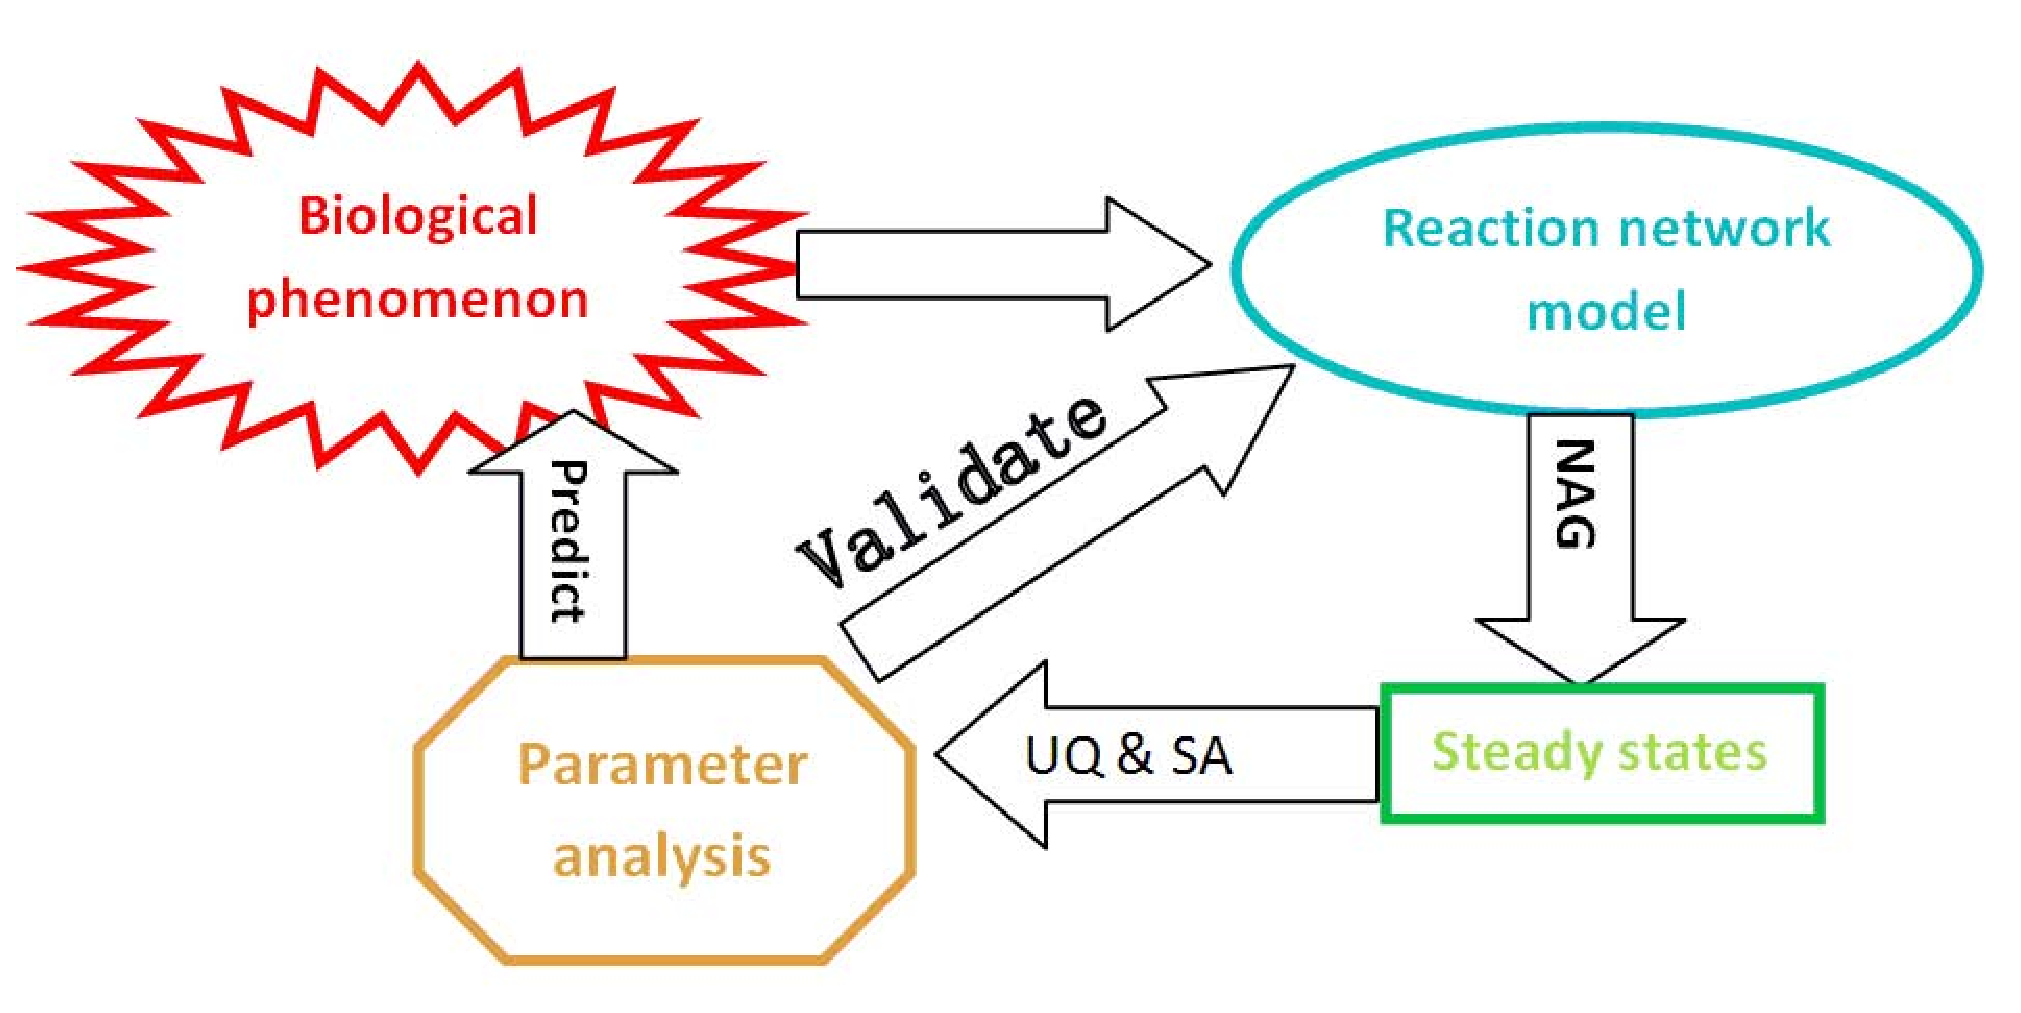
\includegraphics[width=4in,height=2in]{figures/Dia.eps}
\caption{The general approach diagram of different stages in the
analysis process: Numerical algebraic geometry (NAG) provides a
numerical approach to compute all the steady states; Ranking
importance of parameters, which is performed by uncertainty
quantification (UQ) and sensitivity analysis (SA), validates the
mathematical model and gives some medical prediction to the
biological application. } \label{fig:Dia}


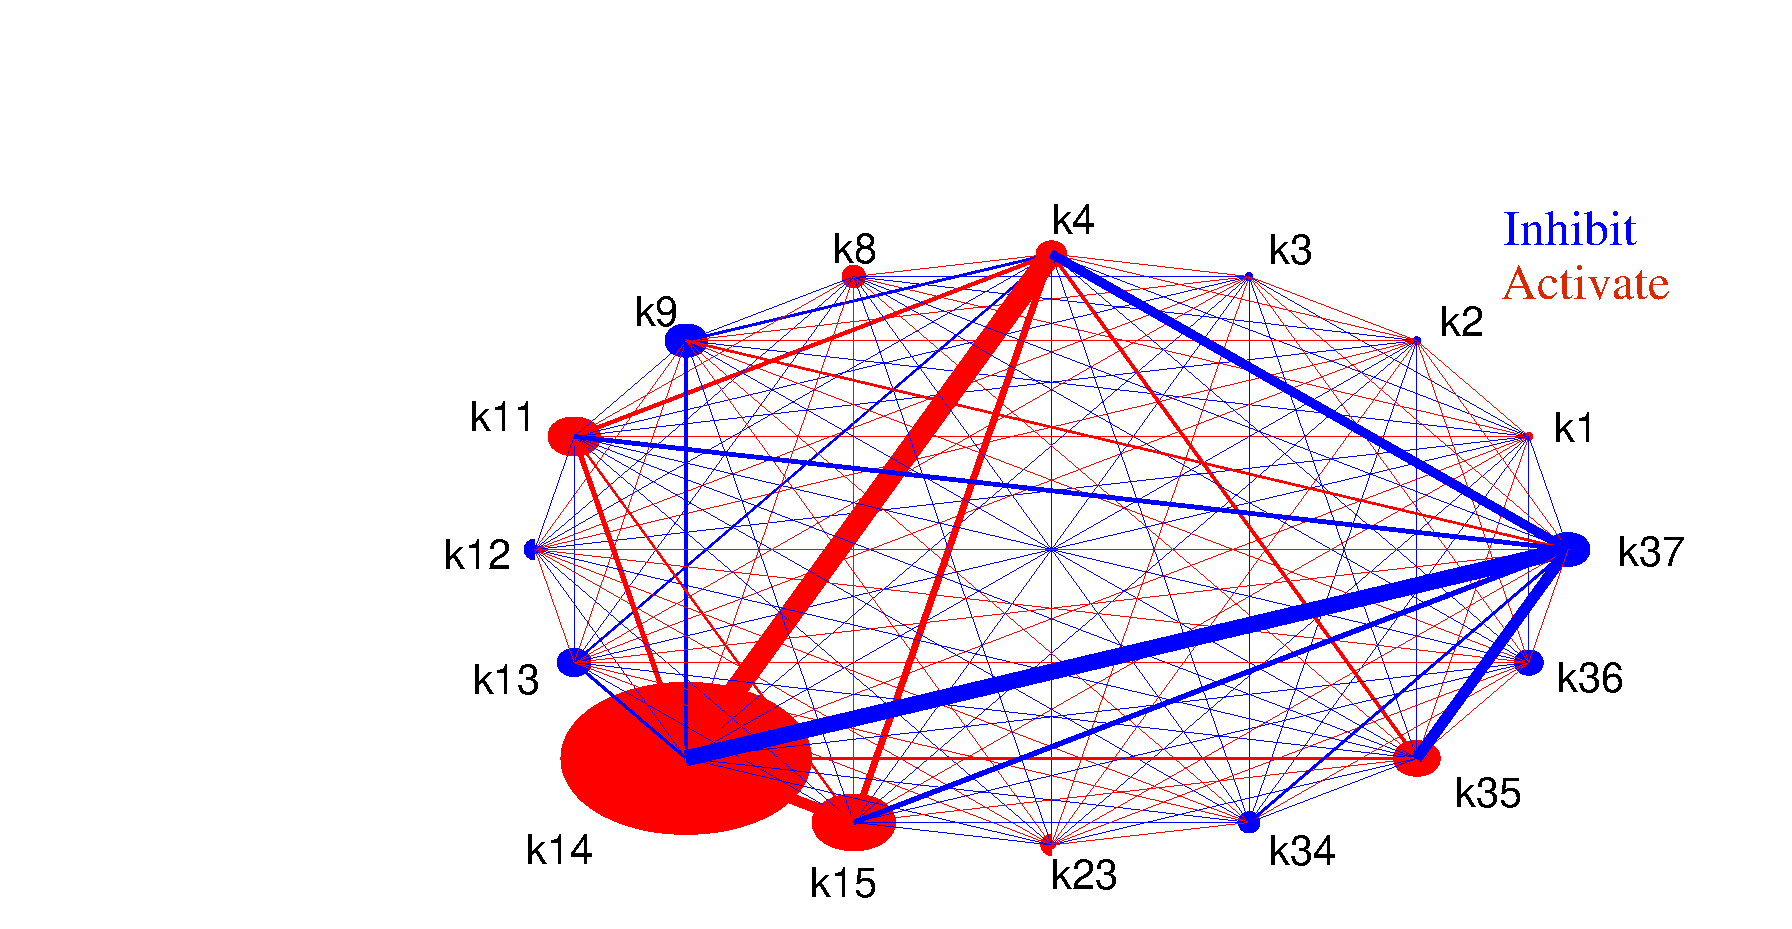
\includegraphics[width=4in,height=3in]{figures/NSA.eps}
\caption{Network graph of importance of reaction rates and the
interaction between pair reactions with respect to total thrombin.
The radius of circles corresponding to reaction rate measures the
rank of sensitivity while the width of lines of any pair of reaction
rates represents rank of their co-sensitivity. The red color
indicates that they play an activate role in generating thrombin
production while the blue color means that they inhibit the
generation of thrombin production. This figure shows that $k_{14}$,
$k_{15}$ and $k_{11}$ are the most sensitive reaction rates in
activating thrombin while $k_{37}$ and $k_{9}$ inhibit thrombin
production. Variance of $k_4$ and $k_{14}$ can play a positive role
in generation of thrombin production, however $k_{37}$ and $k_{14}$
inhibit generation of thrombin production.  } \label{fig:NSA1}


  \end{center}
\end{figure}
\clearpage

\begin{figure}
  \begin{center}
    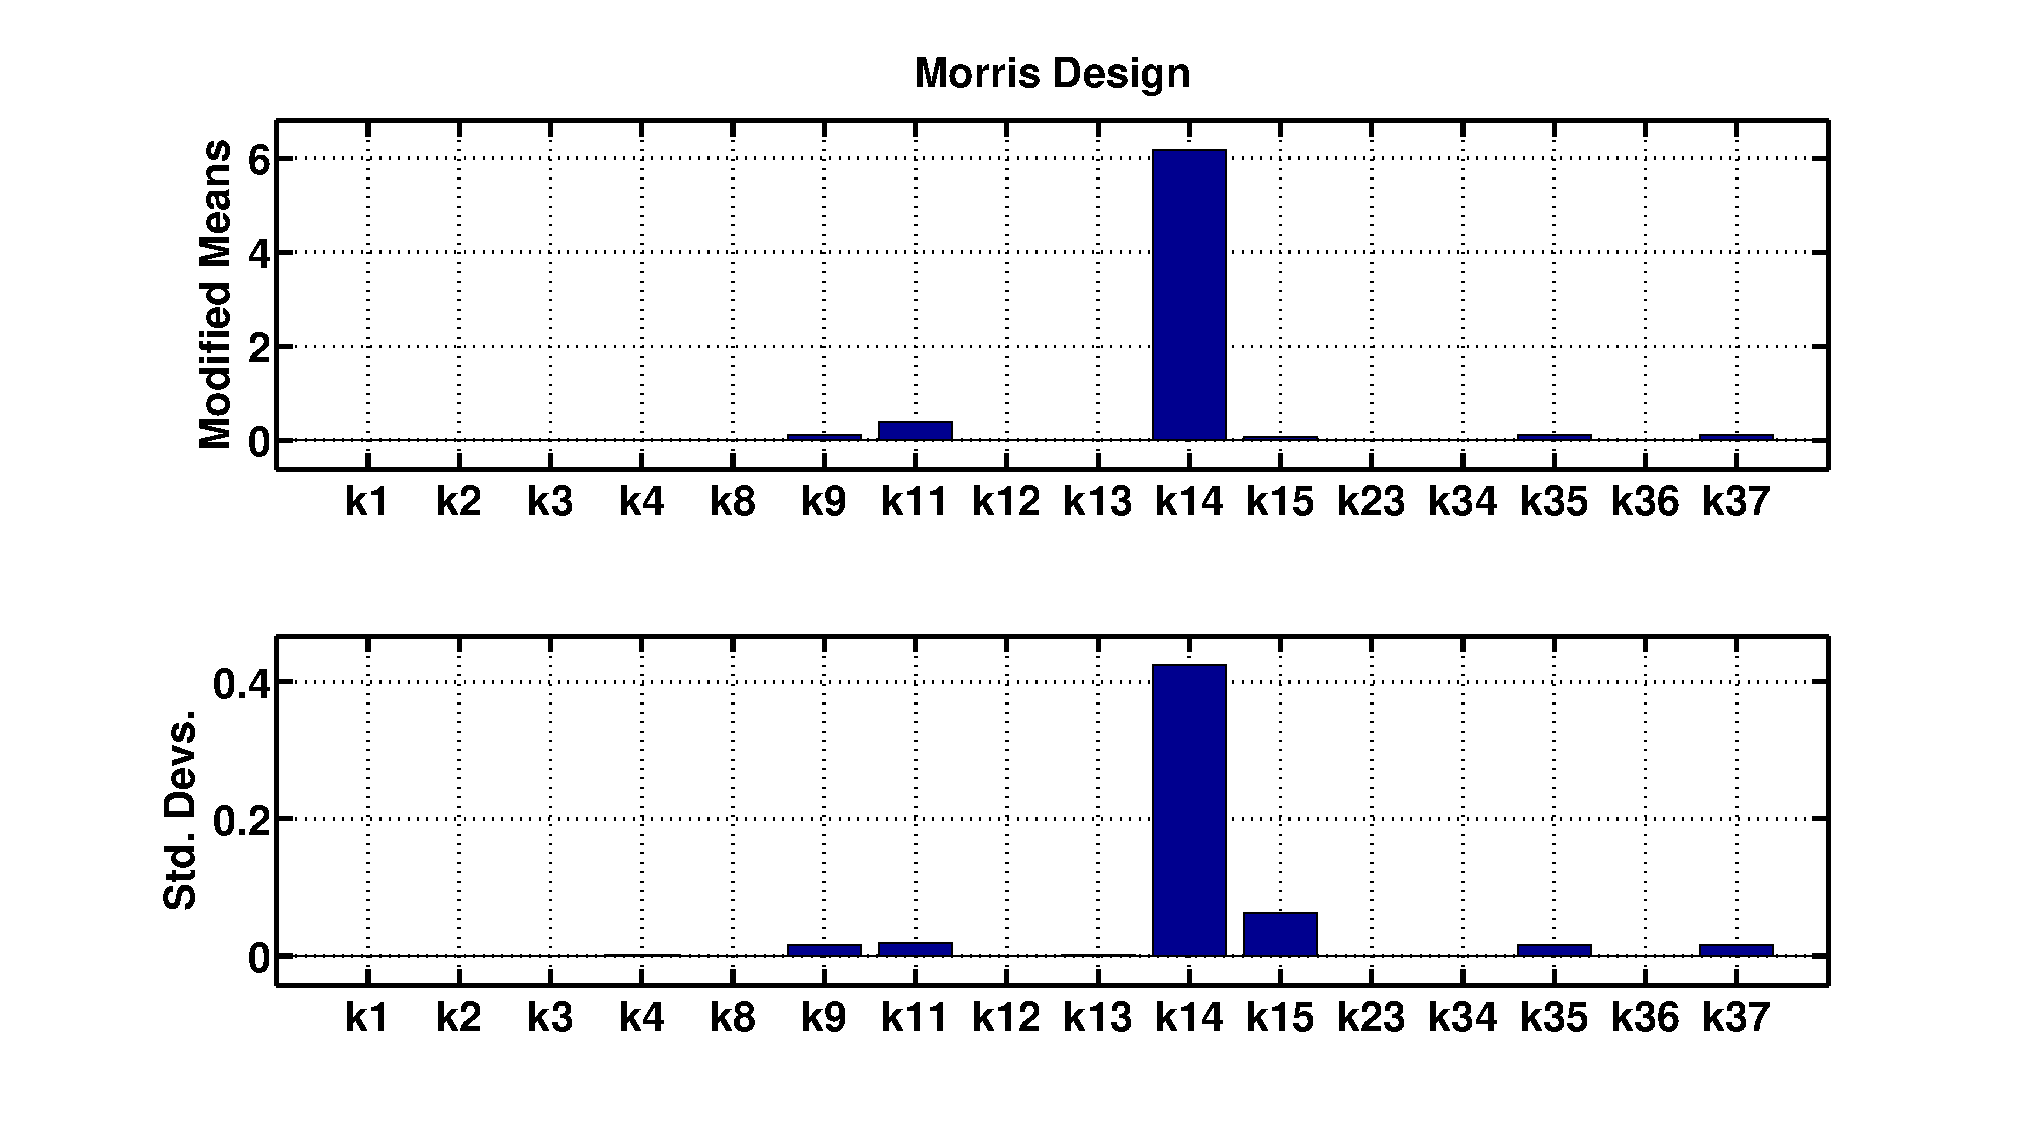
\includegraphics[width=5in]{figures/mean1.eps}
\caption{Modified means and standard deviations based sensitivity
ranking of reaction rates with respect to the total thrombin using
``Morris one at a time'' method. Horizontal axis shows reaction
rates. Vertical axis shows modified means and standard deviations
respectively. This figure indicates that $k_{14}$ has the largest
modified mean and standard deviation. Therefore $k_{14}$ is the most
sensitive to thrombin production. } \label{Fig:mmean}


    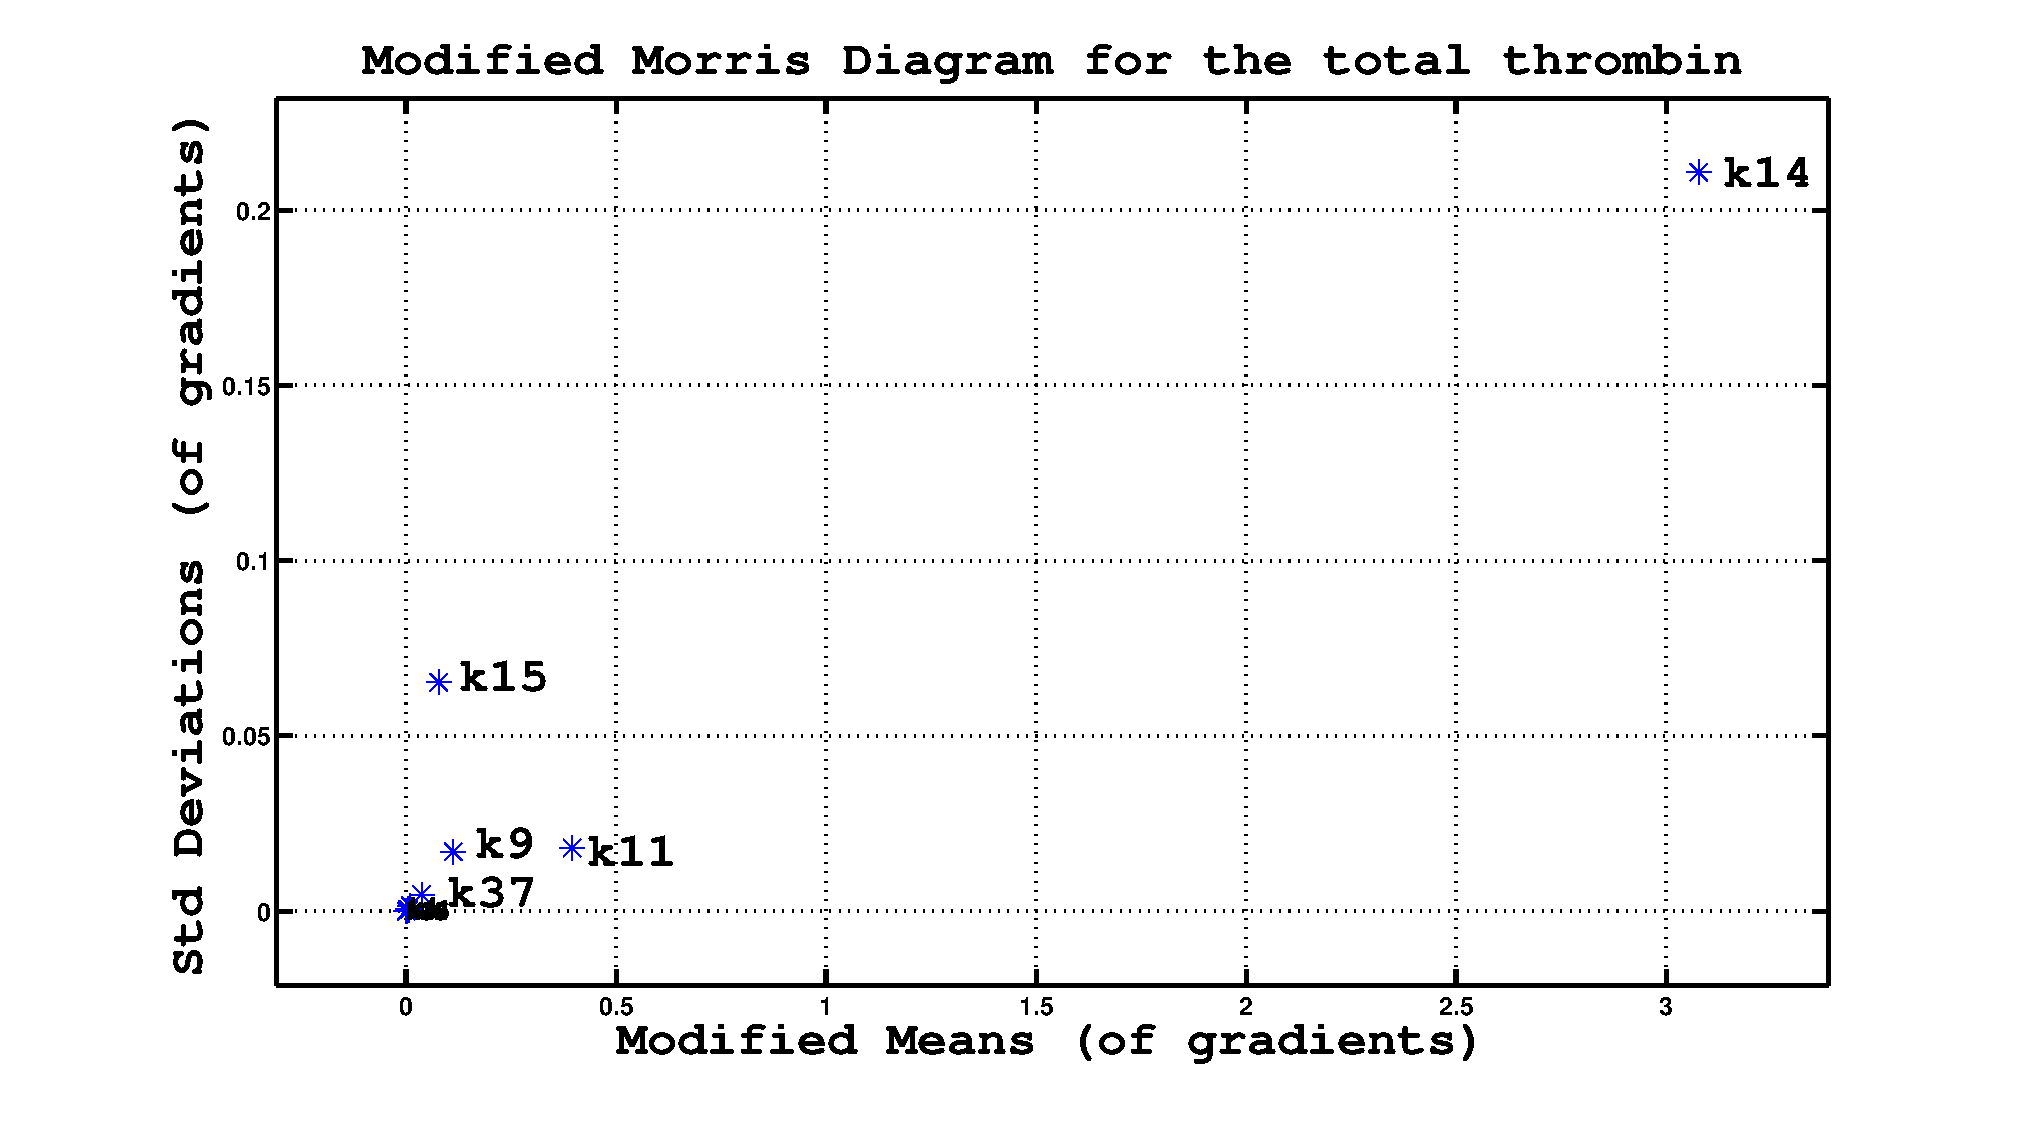
\includegraphics[width=5in]{figures/std.eps}
\caption{Modified Morris diagram on sensitivity ranking of reaction
rates with respect to the total thrombin. Ranks of sensitivity for
individual reaction rates are determined by their distance from the
origin. From this figure, the five most sensitive reaction rates are
$k_{14}$, $k_{15}$,  $k_{11}$, $k_{9}$ and $k_{37}$. The other
reaction rates cluster together due to the same magnitude of
sensitivity. } \label{Fig:std}


  \end{center}
\end{figure}

\begin{figure}
  \begin{center}

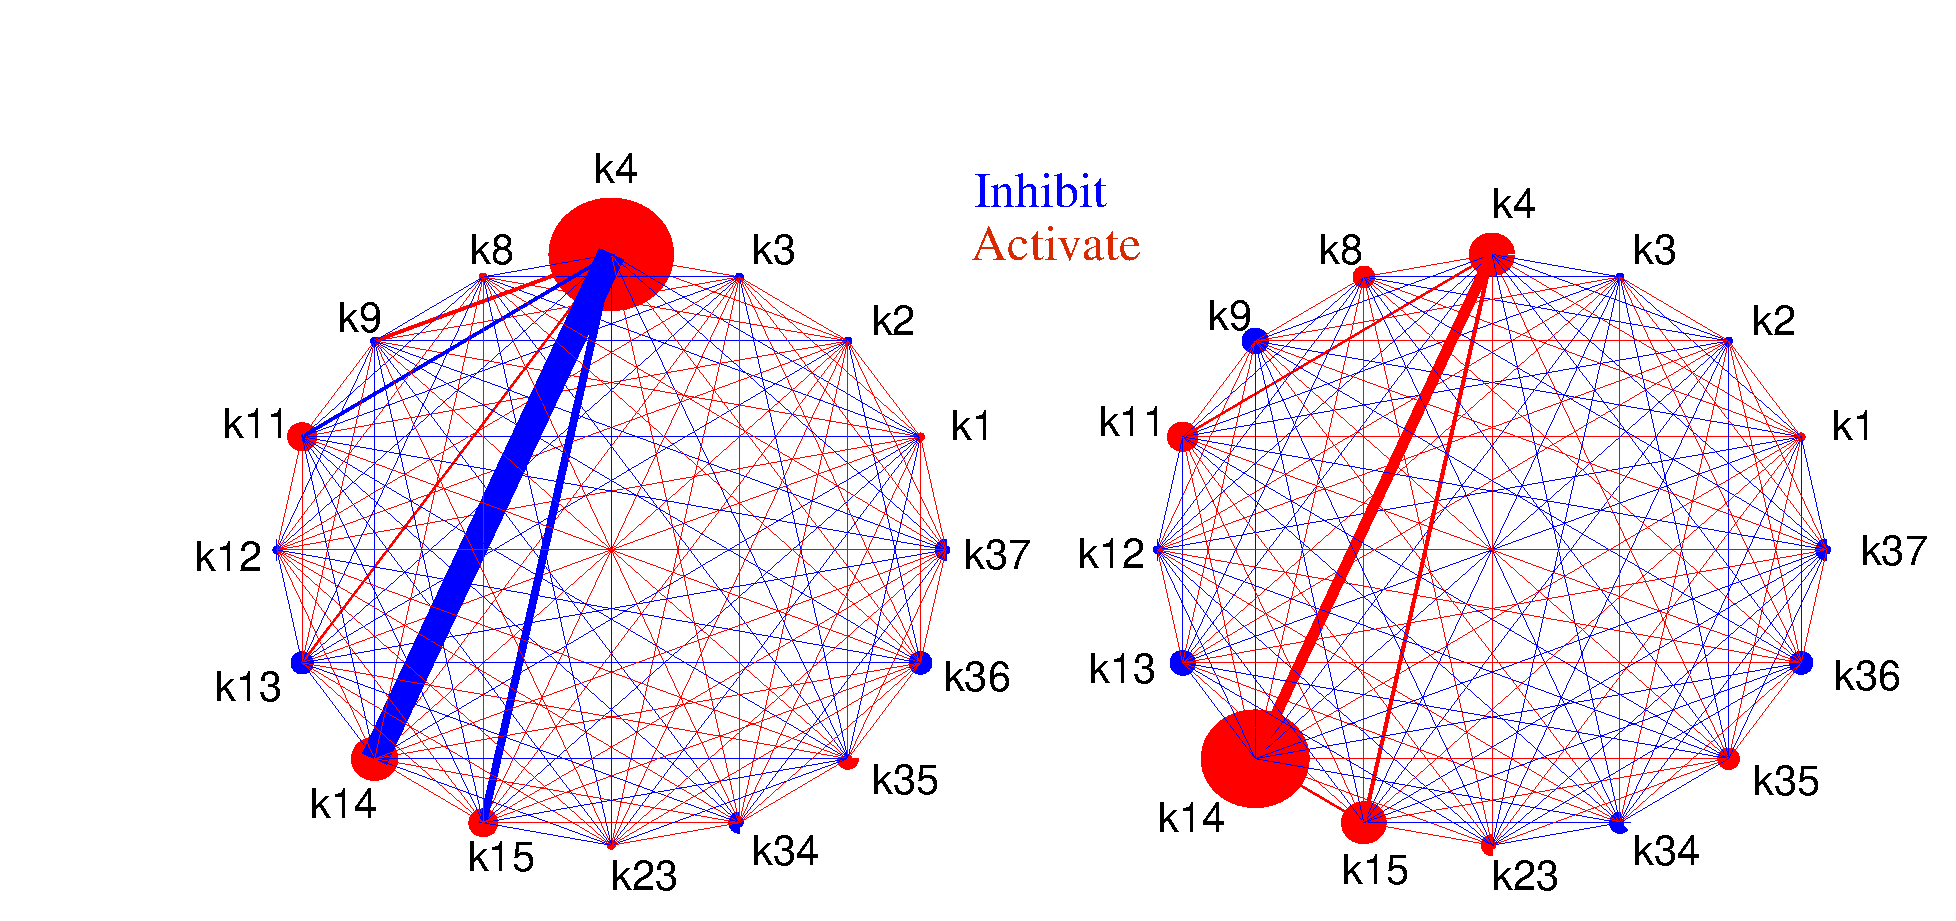
\includegraphics[width=5in,height=2.5in]{figures/nsarb33.eps}
\caption{Network graph of importance of reaction rates and the
interaction between reaction rates with respect to IXa=VIIIa
($x_{33}$) and IXa=ATIII ($x_{30}$) respectively. The same legend is
used with Figure 1. This figure shows that the rank of sensitivity
varices with respect to different output variables. }
\label{fig:NSA}


  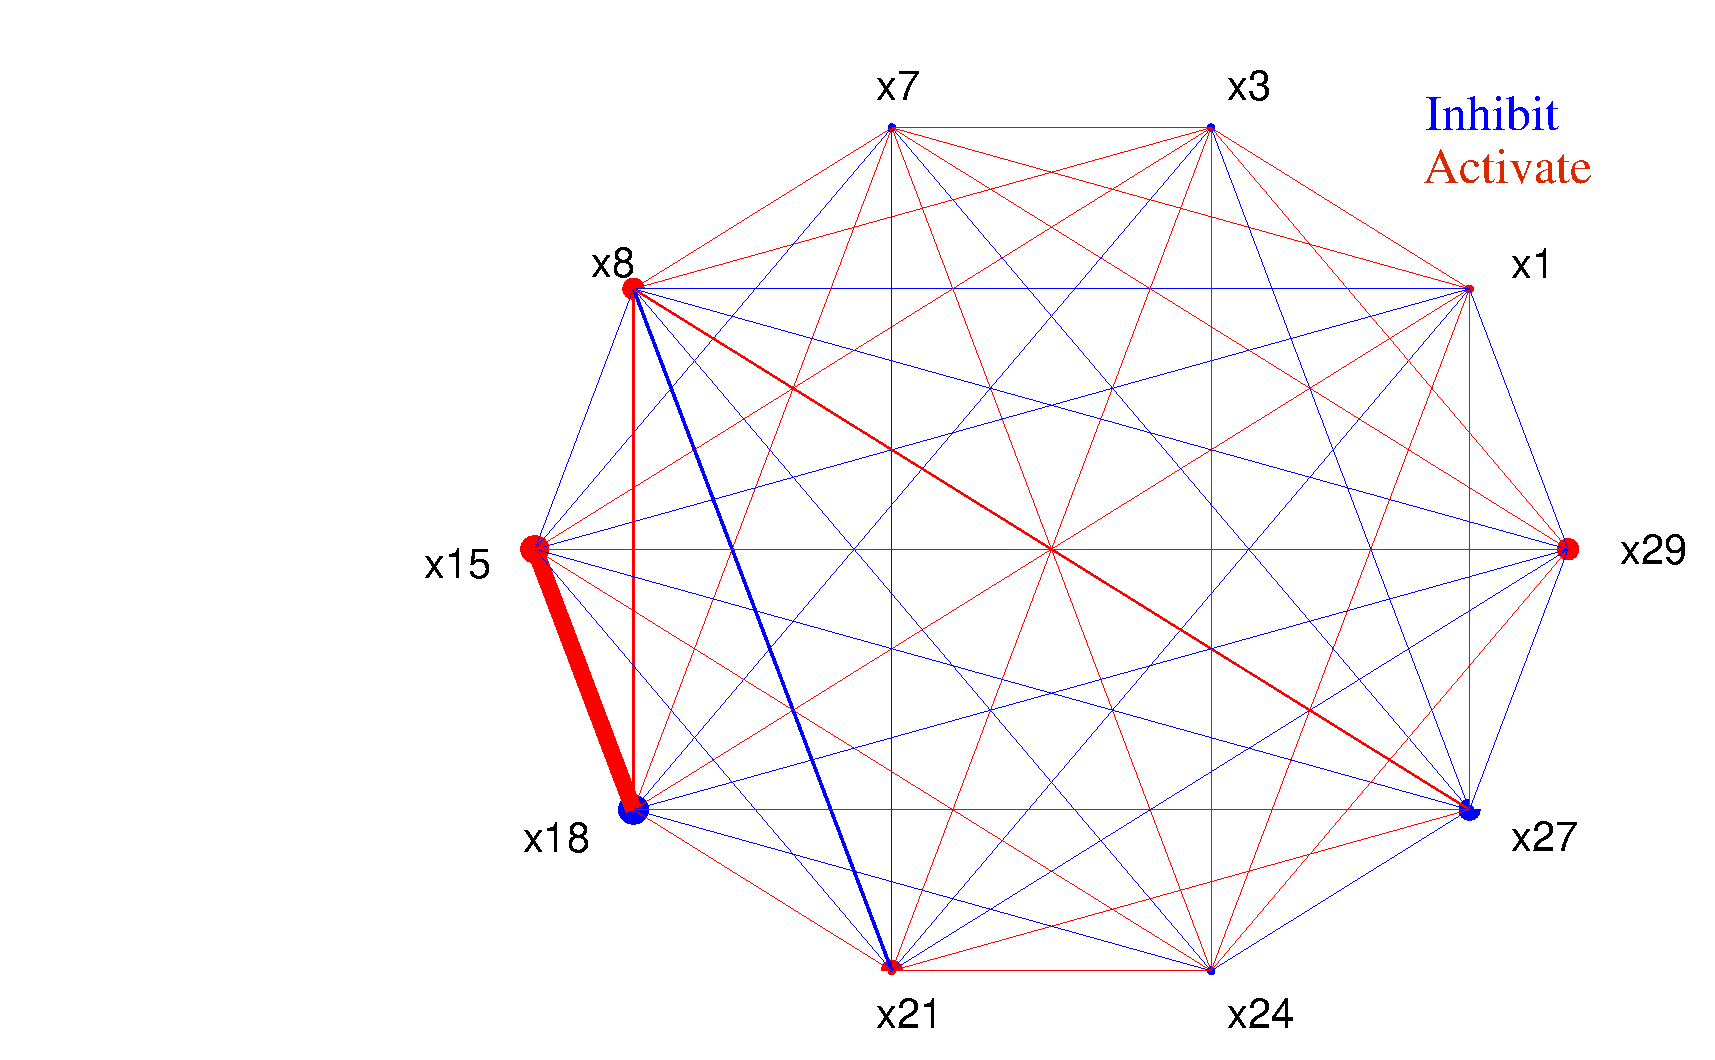
\includegraphics[width=4in]{figures/nsaic.eps}
\caption{Network graph of importance of initial condition and the
interaction between pair components with respect to total thrombin.
See the legend in Figure 3. This figure shows that factor X
($x_{15}$) is the most sensitive reaction component in activating
thrombin while TFPI ($x_{18}$) inhibits thrombin production.
Moreover, their variance can play a positive role in generation of
thrombin production.} \label{Fig:nsaic}


  \end{center}
\end{figure}

\begin{figure}
  \begin{center}

  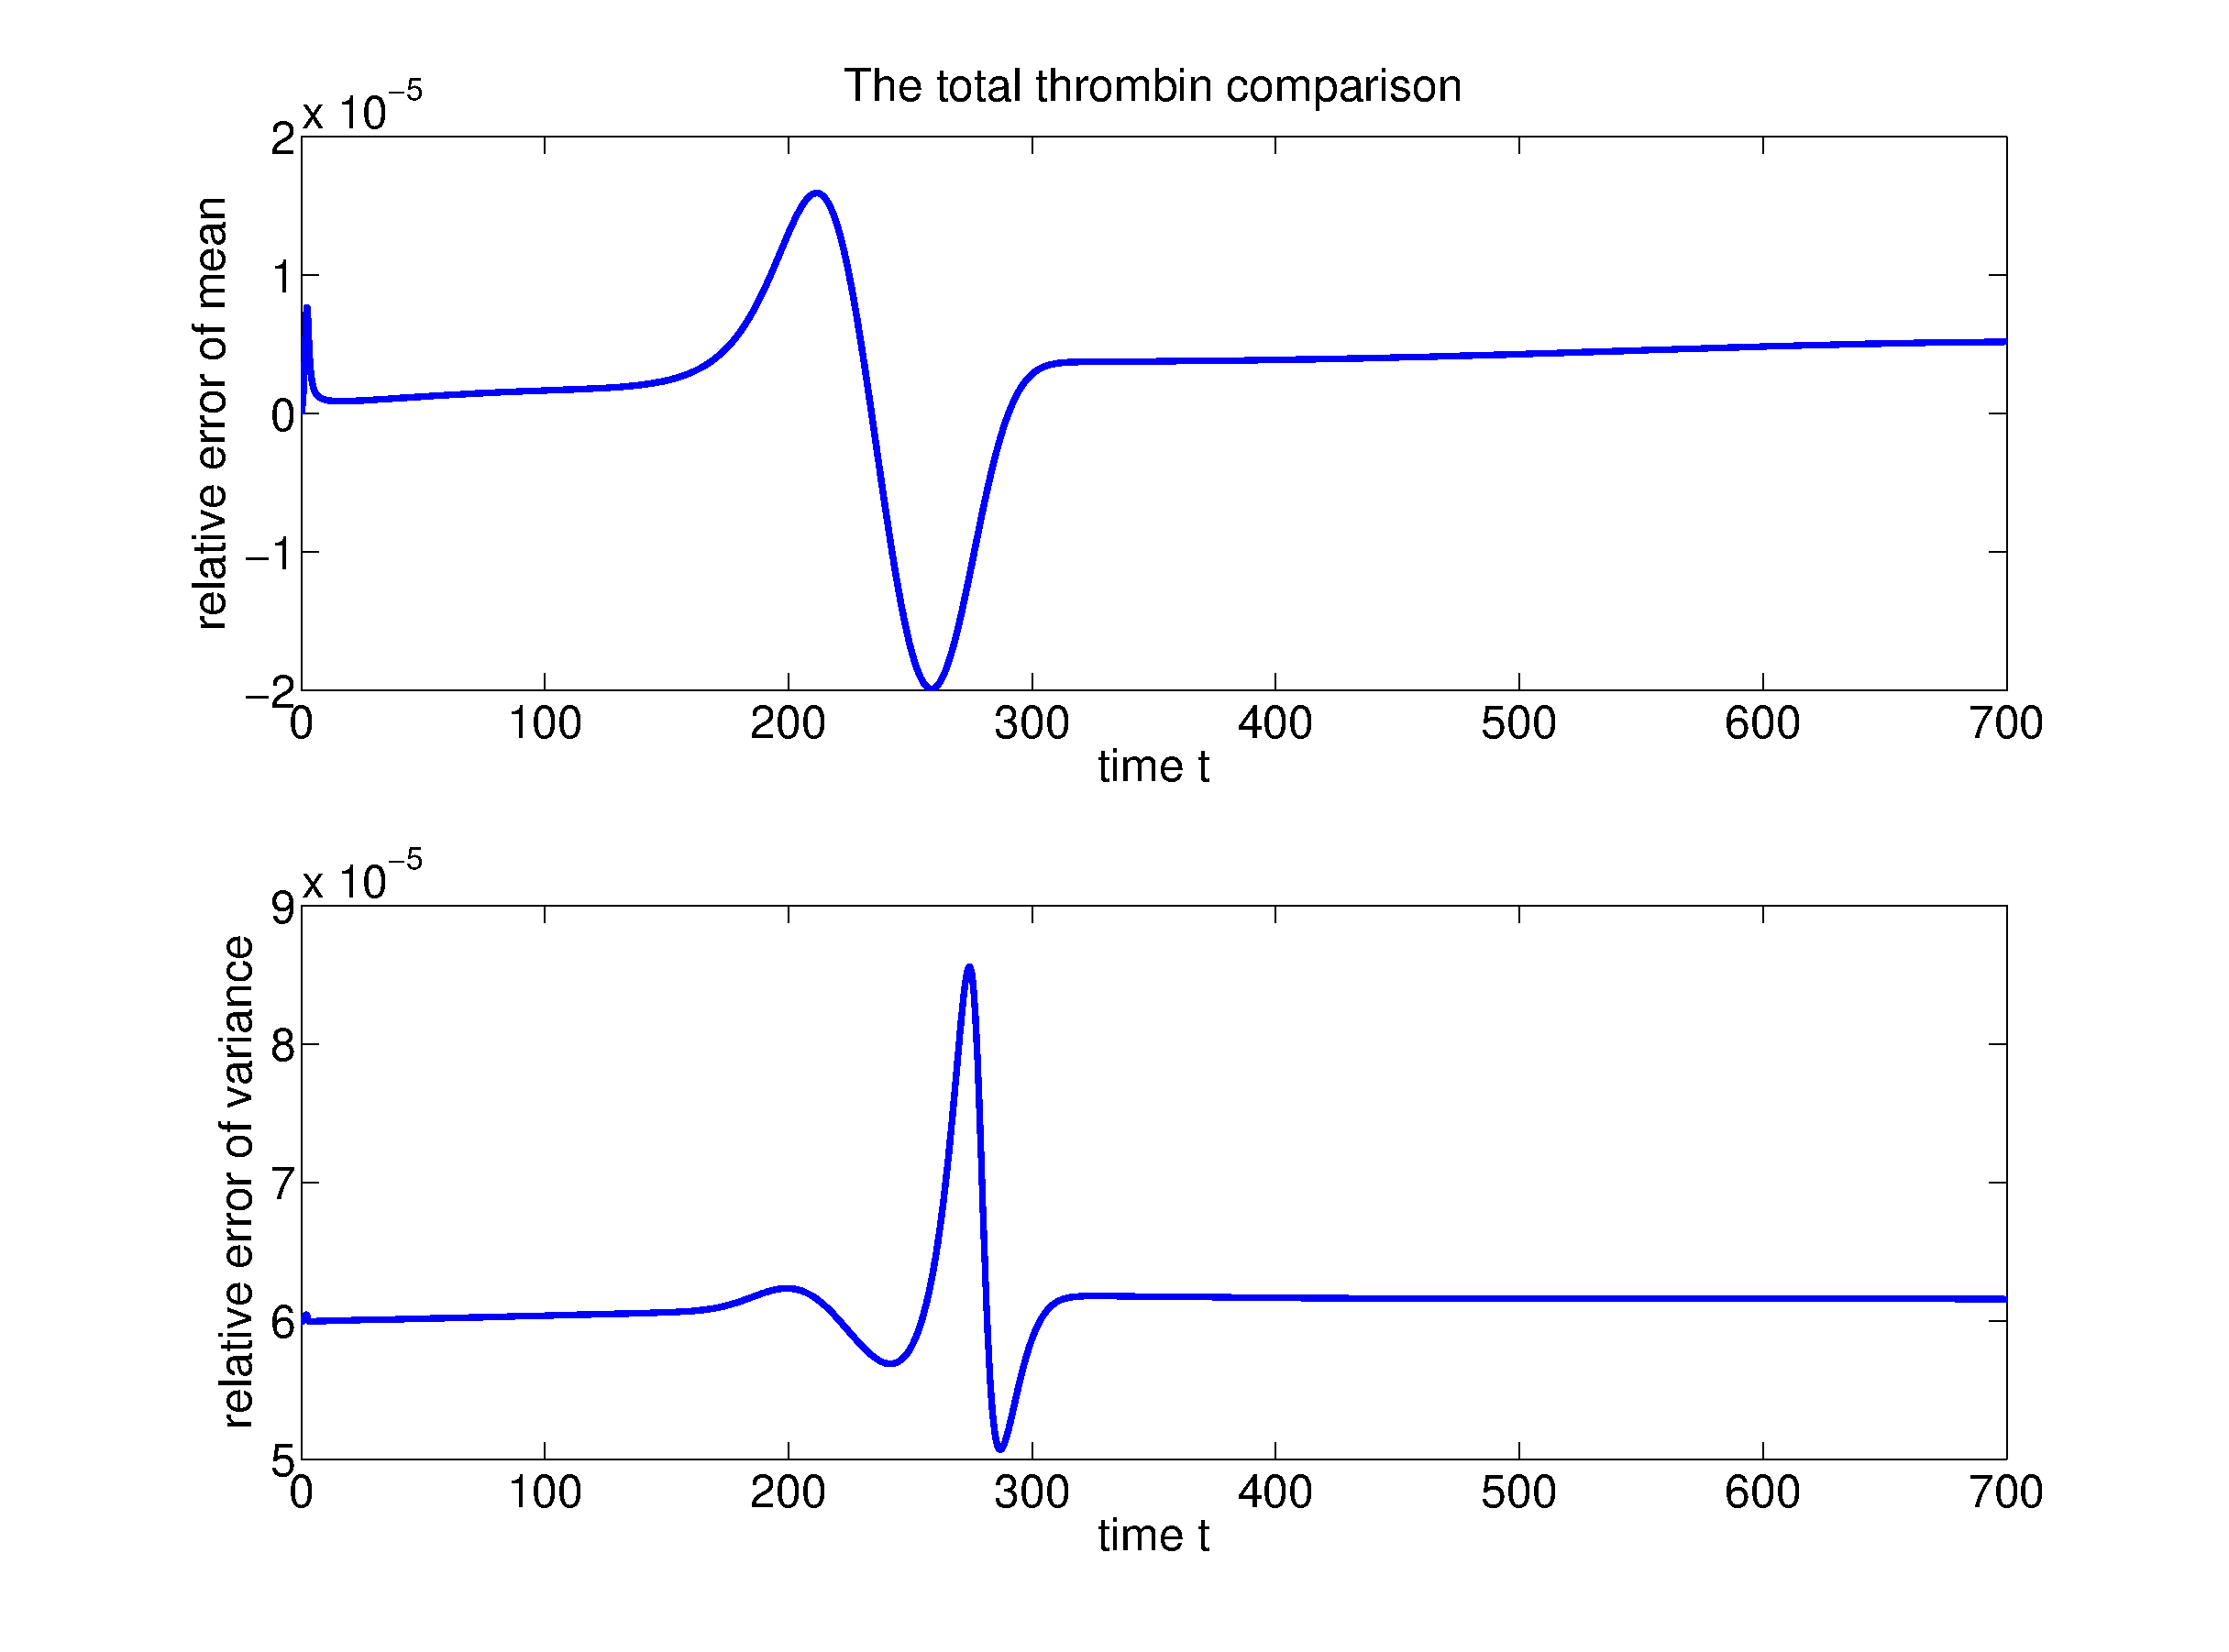
\includegraphics[width=5in]{figures/comp.eps}
\caption{The Difference of mean and variance of the total thrombin
obtained by SGPCM ($545$ points) and MC ($1000$ points). The figure
shows that the results of two methods are same under small
tolerance. %The peaks of two figures because the variance of
 %total thrombin is relatively fast at this point (See Figure 8).
 } \label{Fig:comp}

  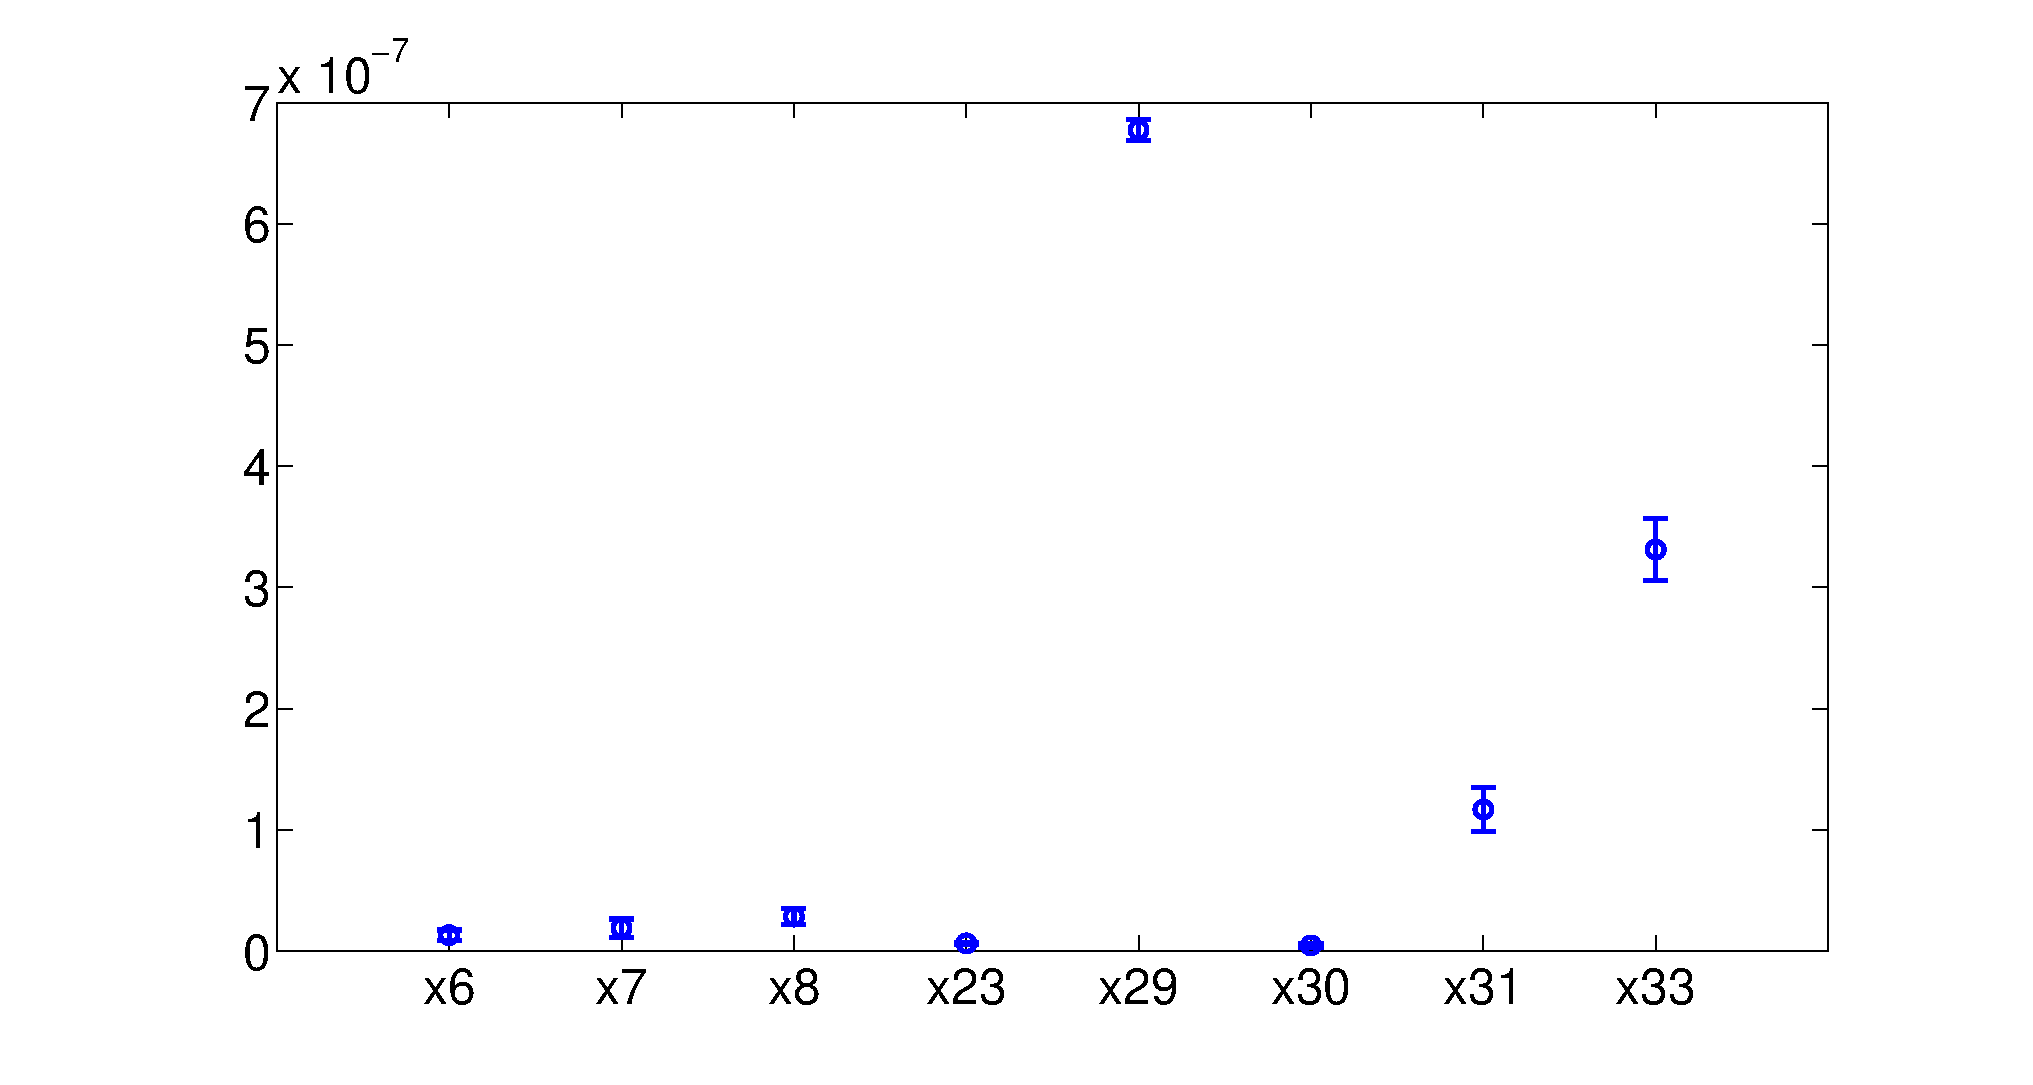
\includegraphics[width=5in]{figures/steady.eps}
\caption{Mean and error bar of steady state solutions whose
magnitude are greater than $10^{-10}$. Horizontal axis is reaction
rates. This figure shows confidence intervals of each reaction
rates.} \label{Fig:steady}

  \end{center}
\end{figure}

\begin{figure}
  \begin{center}
  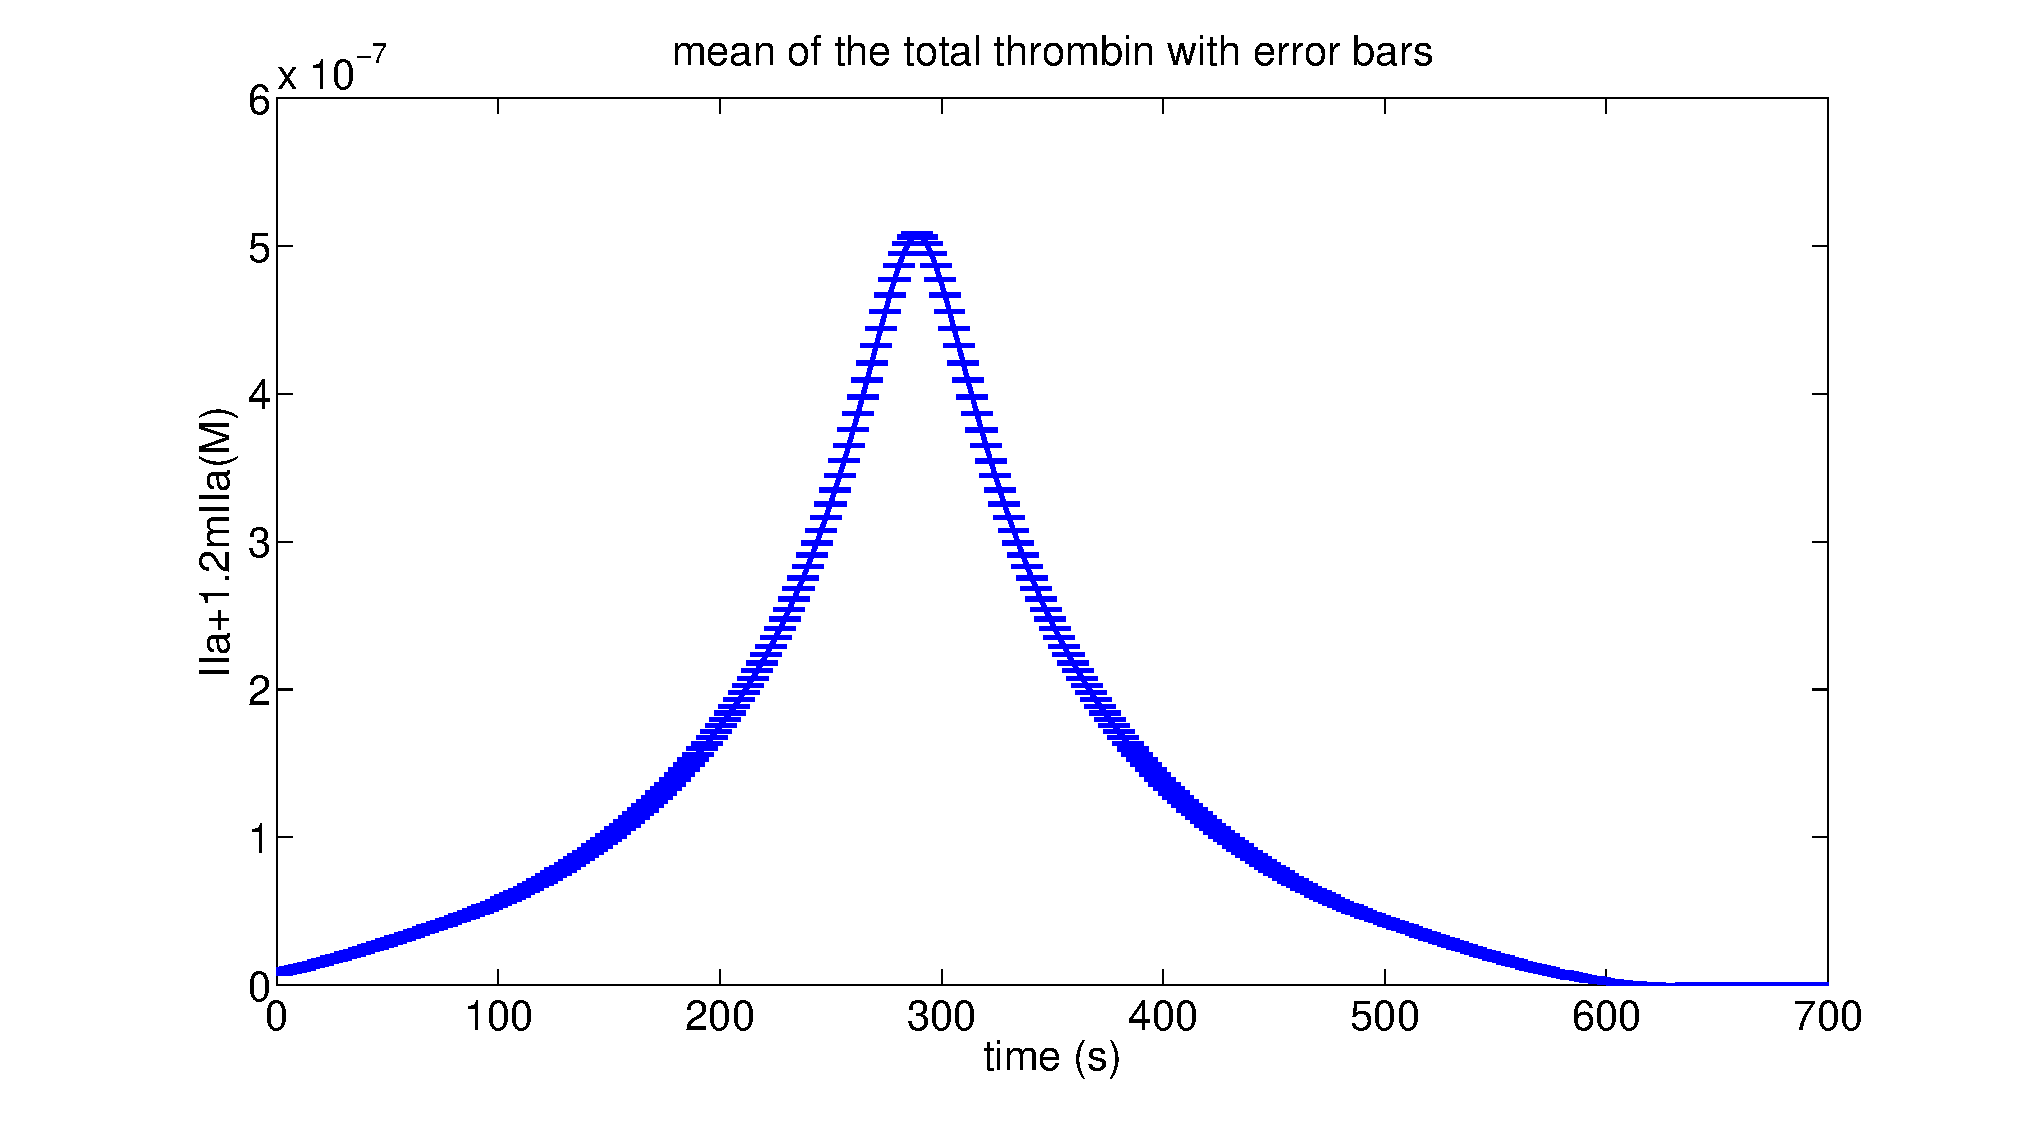
\includegraphics[width=5in]{figures/mean.eps}
\caption{The mean and error bar of the total thrombin along the
solution by time marching. Error bars show the confidence intervals
of reaction rates along the curve. }\label{Fig:mean}


  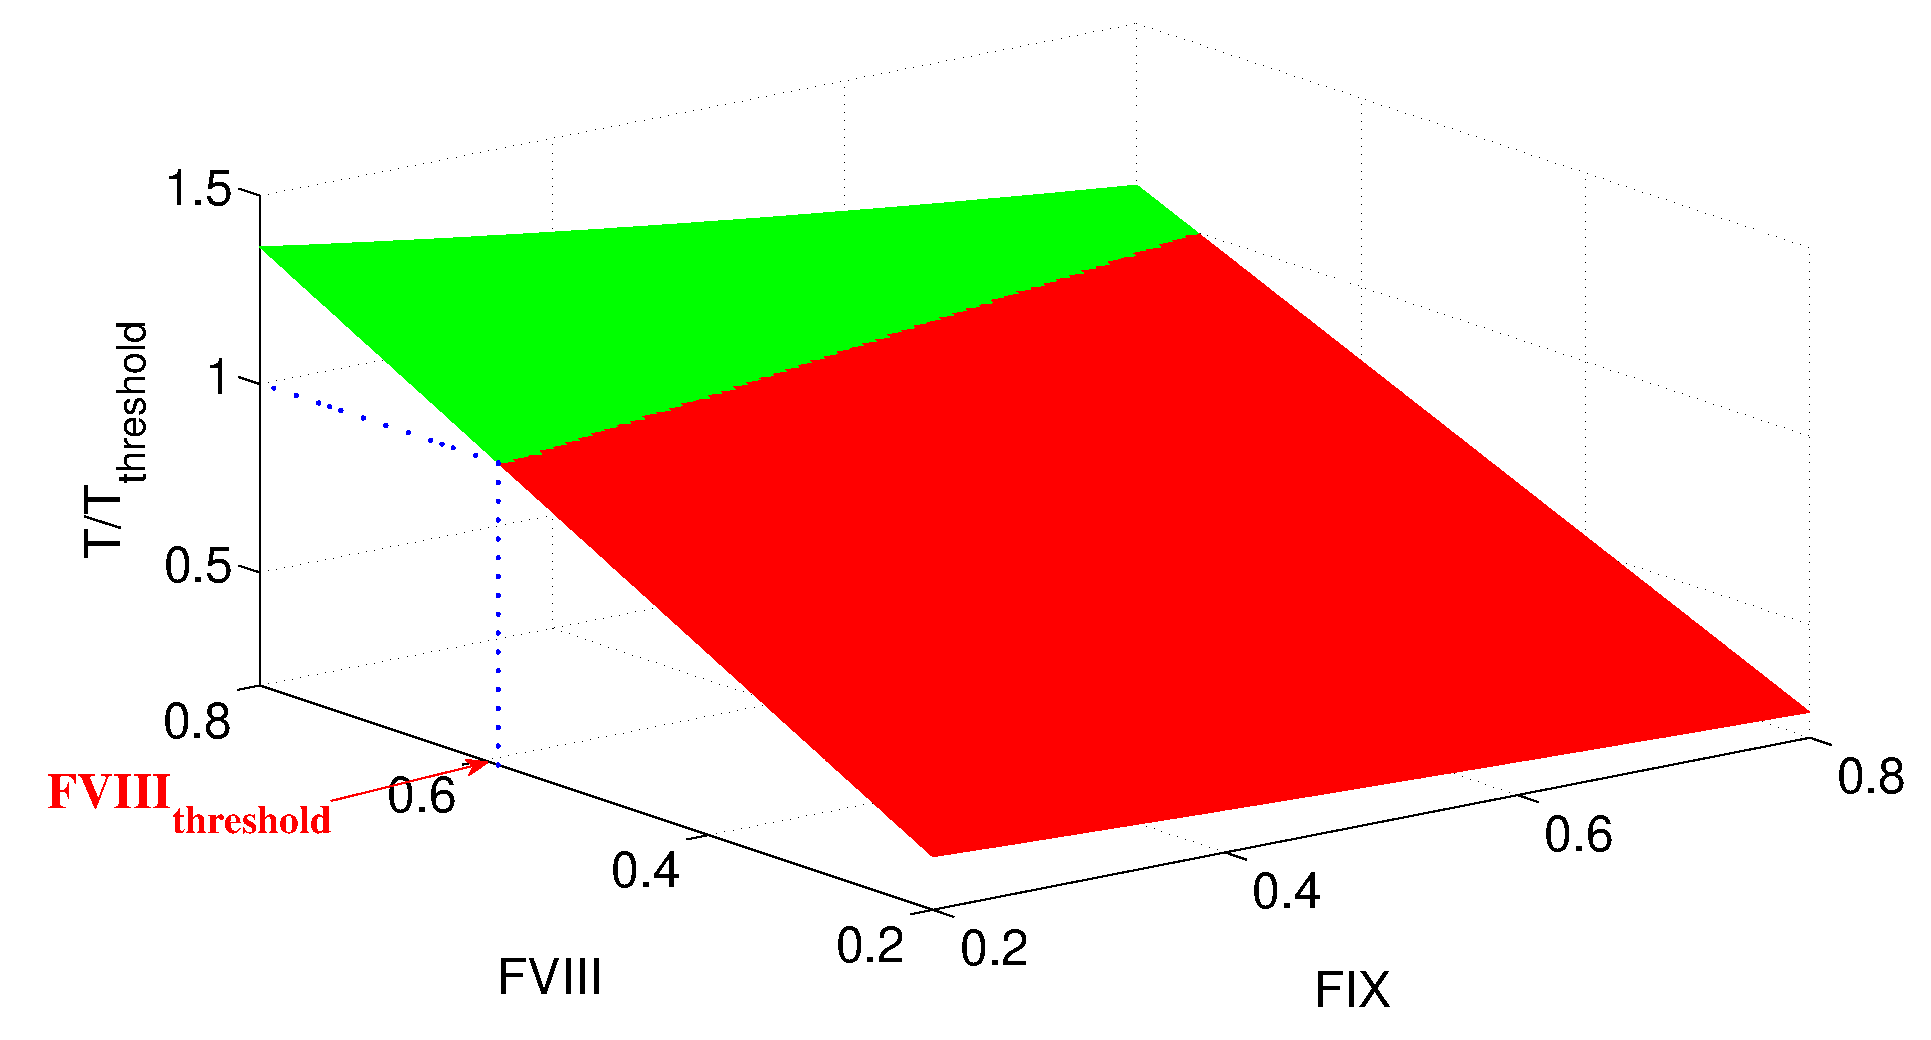
\includegraphics[width=5in]{figures/F89.eps}
\caption{The total thrombin \textit{v.s.} factors VIII (FVIII) and
IX (FIX). $T_{threshold}$ stands for the threshold  value of
thrombin. The red portion of the plane means the total thrombin (T)
is smaller than $T_{threshold}$ while the green portion means the
total thrombin is greater than $T_{threshold}$. This figure shows
that the threshold of factor VIII is 4.7 \% of normal value, and
that the total thrombin is greater than $T_{theshold}$ when factor
VIII is greater than $FVIII_{theshold}$ regardless of factor IX
concentration when it's in the assume range.}\label{Fig:F89}


  \end{center}
\end{figure}

\begin{figure}
  \begin{center}
  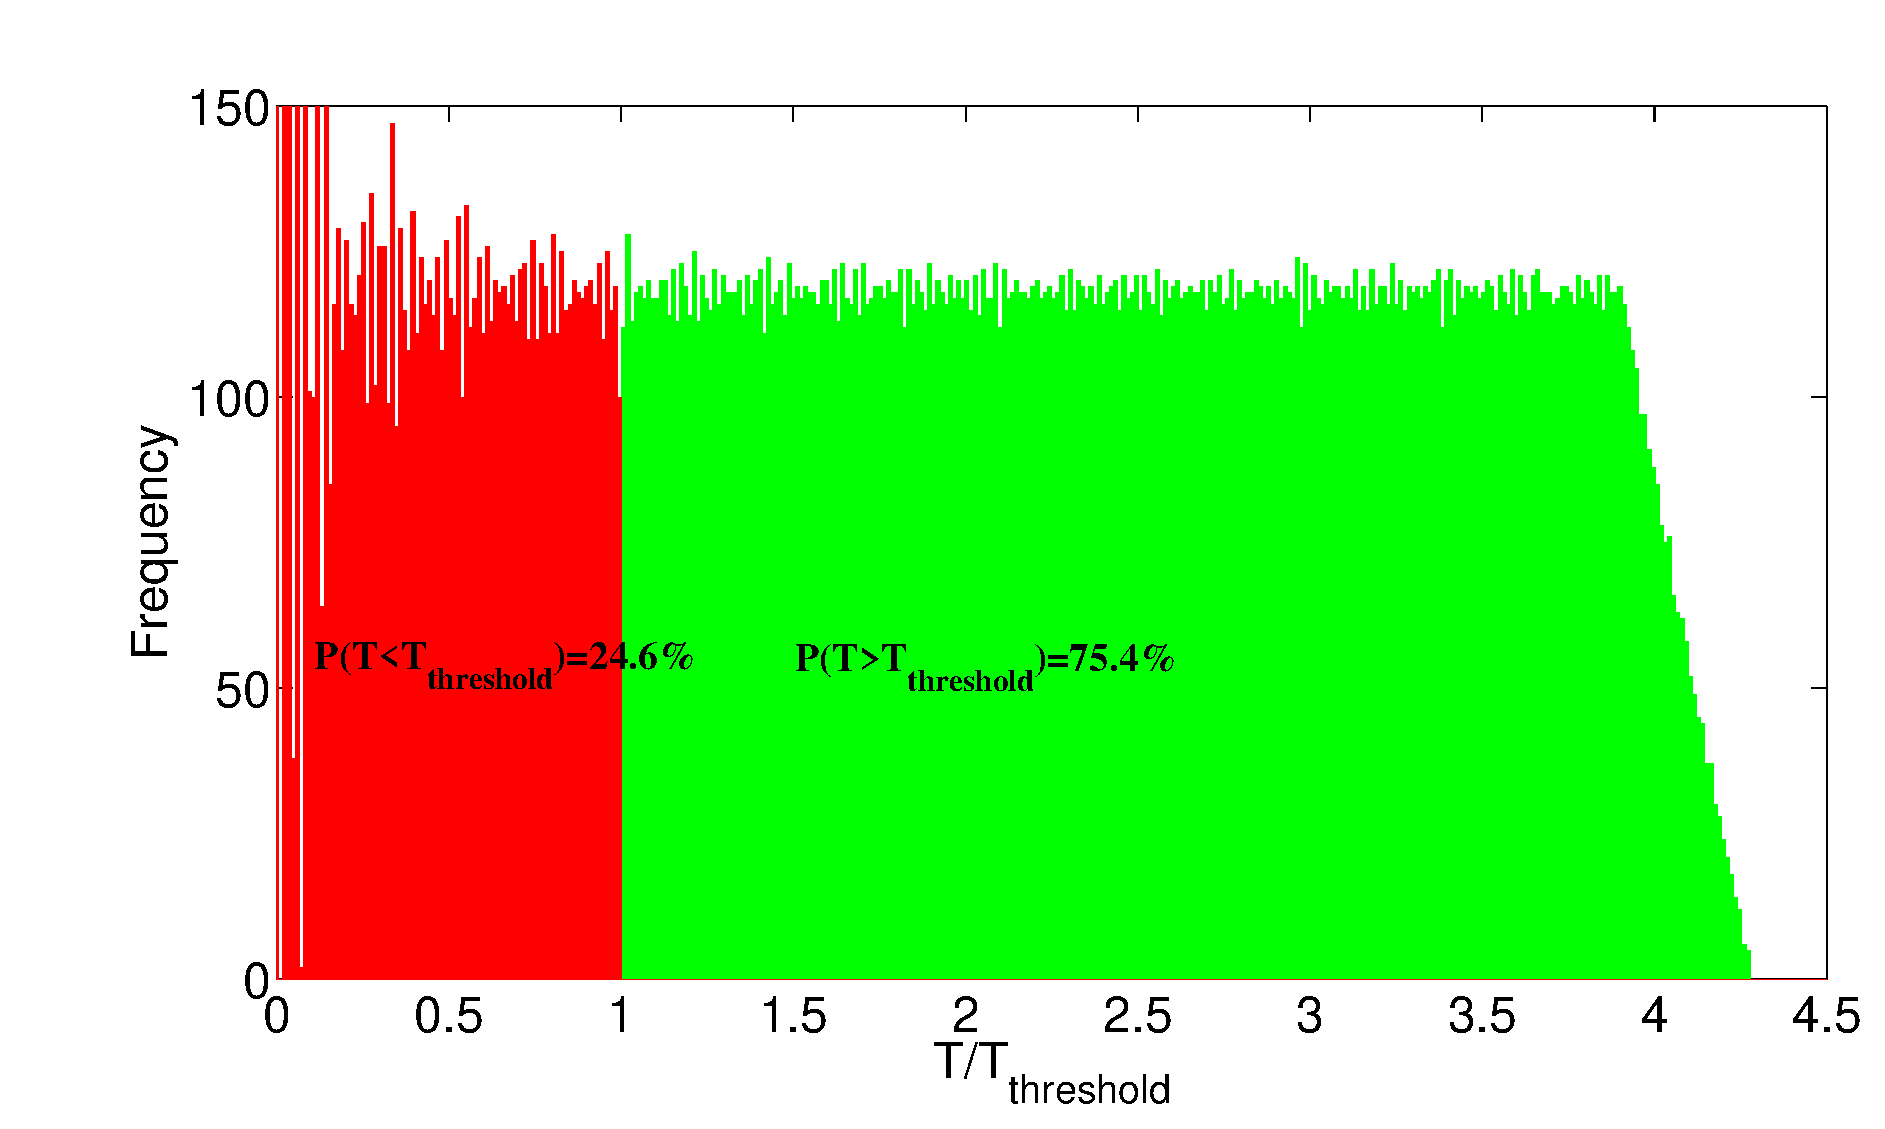
\includegraphics[width=5in]{figures/F89hist.eps}
\caption{Histogram of the total thrombin. The probability that the
total thrombin is greater than $T_{threshold}$ is
75.4\%.}\label{Fig:F89hist}

  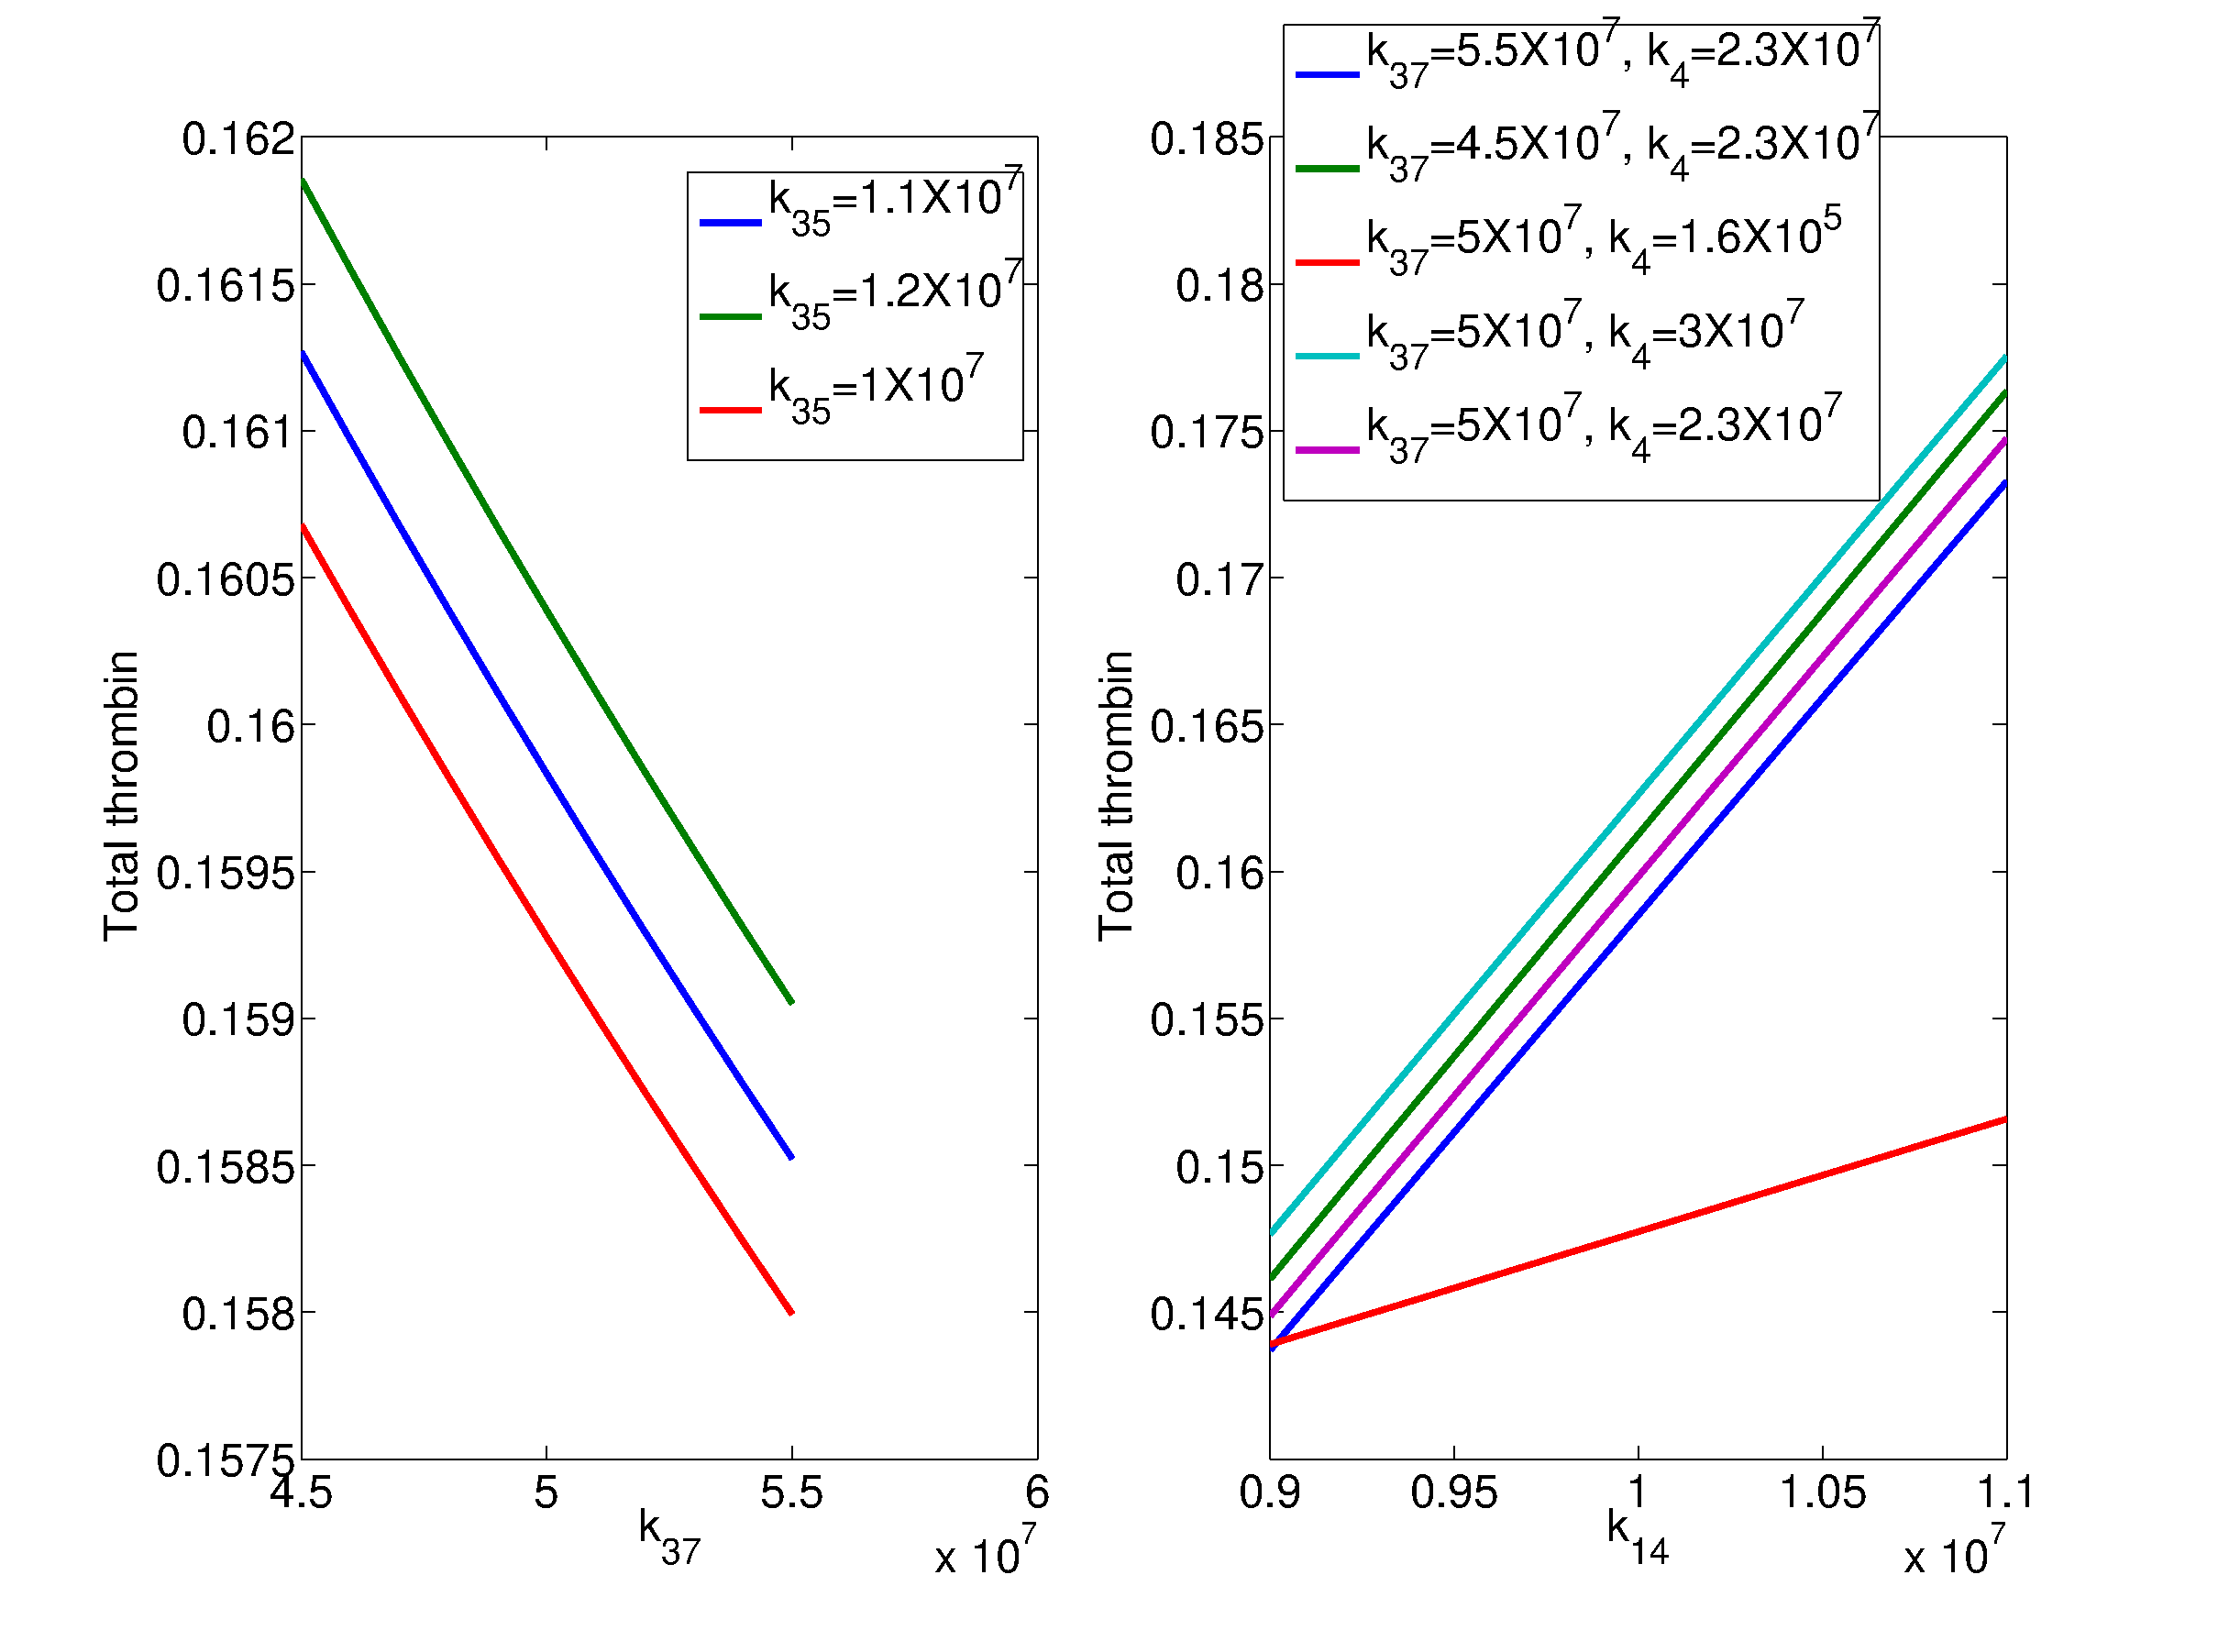
\includegraphics[width=5in,height=3in]{figures/rv.eps}
\caption{The total thrombin \textit{v.s.} reaction rates $k_{37}$
and $k_{14}$. $k_{37}$ inhibits the generation of total thrombin as
it increases. $k_{35}$ plays a negative role in the effect of
$k_{37}$. $k_{14}$ activates the generation of total thrombin as it
increases. $k_{37}$ and $k_4$ play negative and positive roles in
the effect of $k_{14}$ respectively.}\label{Fig:RV}

  \end{center}
\end{figure}
\clearpage

\begin{figure}
  \begin{center}
  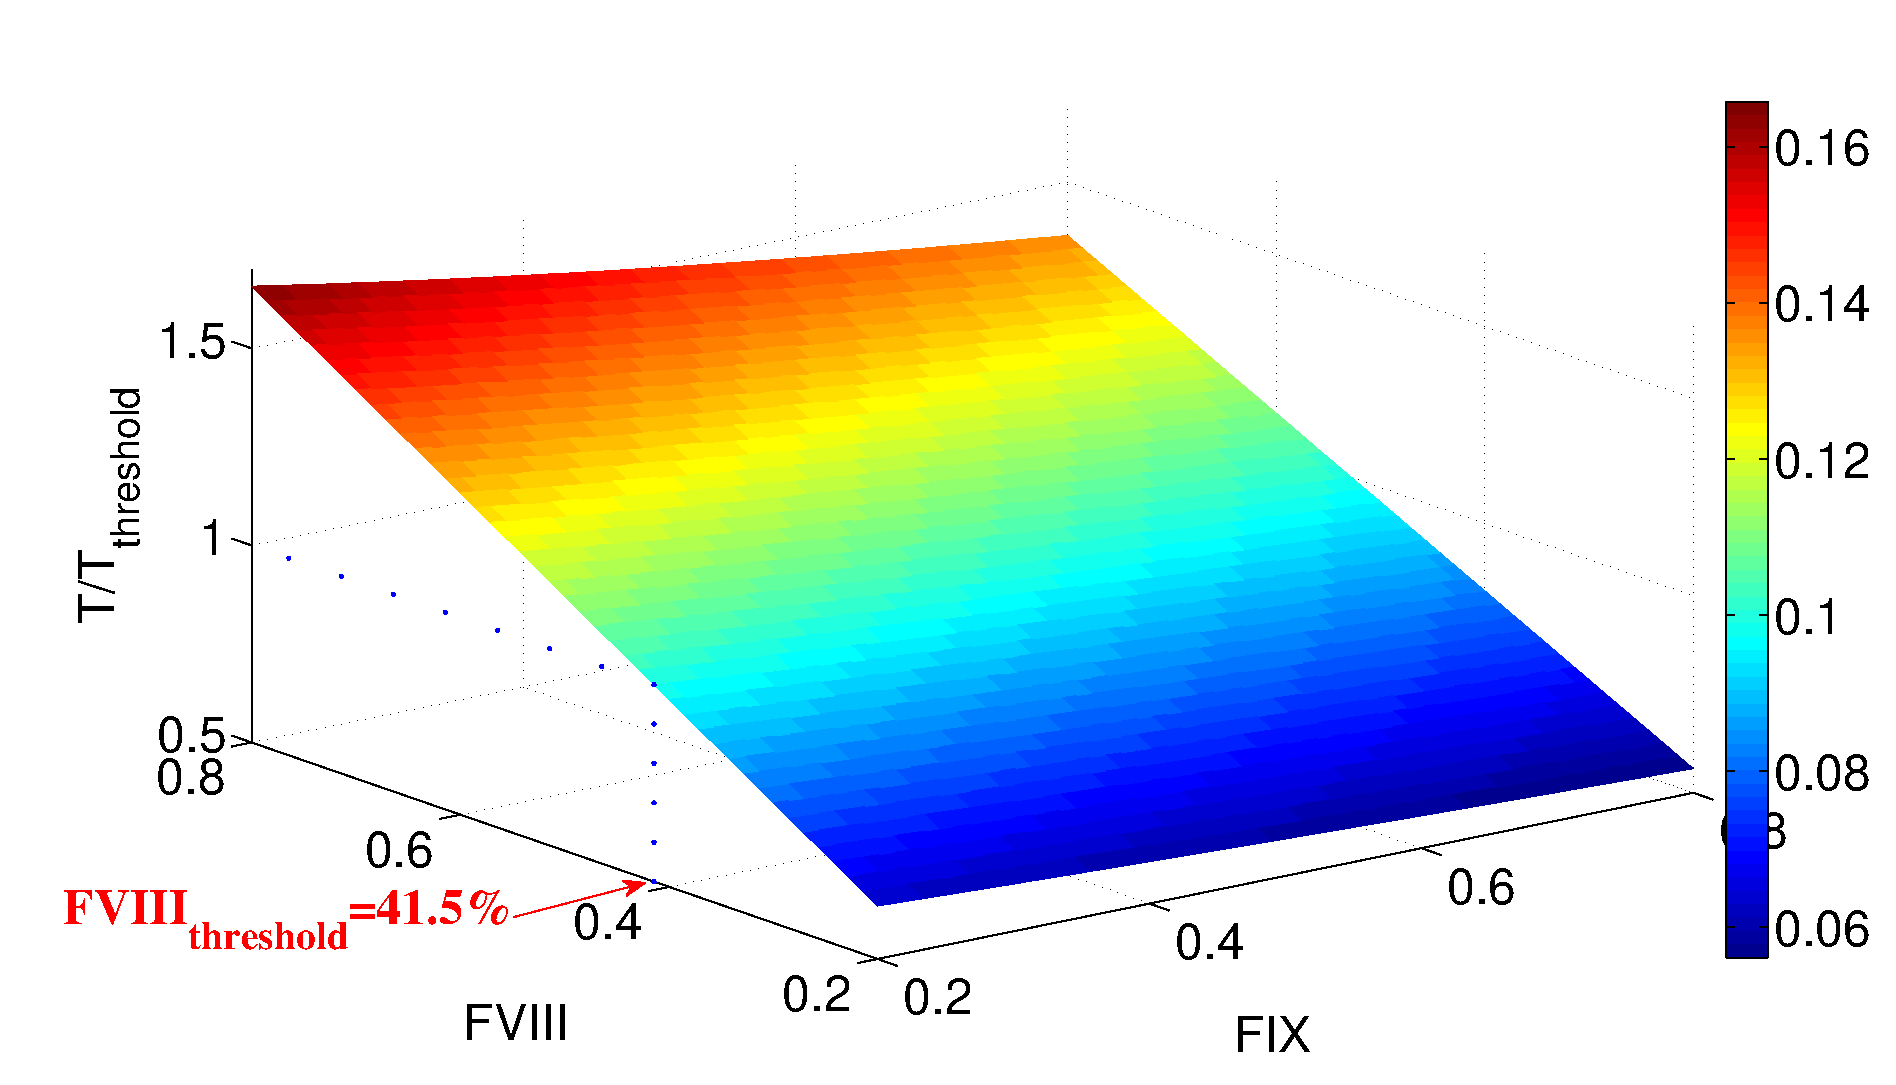
\includegraphics[width=5in]{figures/F89m.eps}
\caption{The mean of the total thrombin of sampling points of
$k_{14}$ and factor X, which vary from 100\%-200\% of their normal
values. The color means the variance of the total thrombin. This
figure shows that the threshold of factor VIII is decreased to 3.3\%
of normal value.}\label{Fig:F89m}

  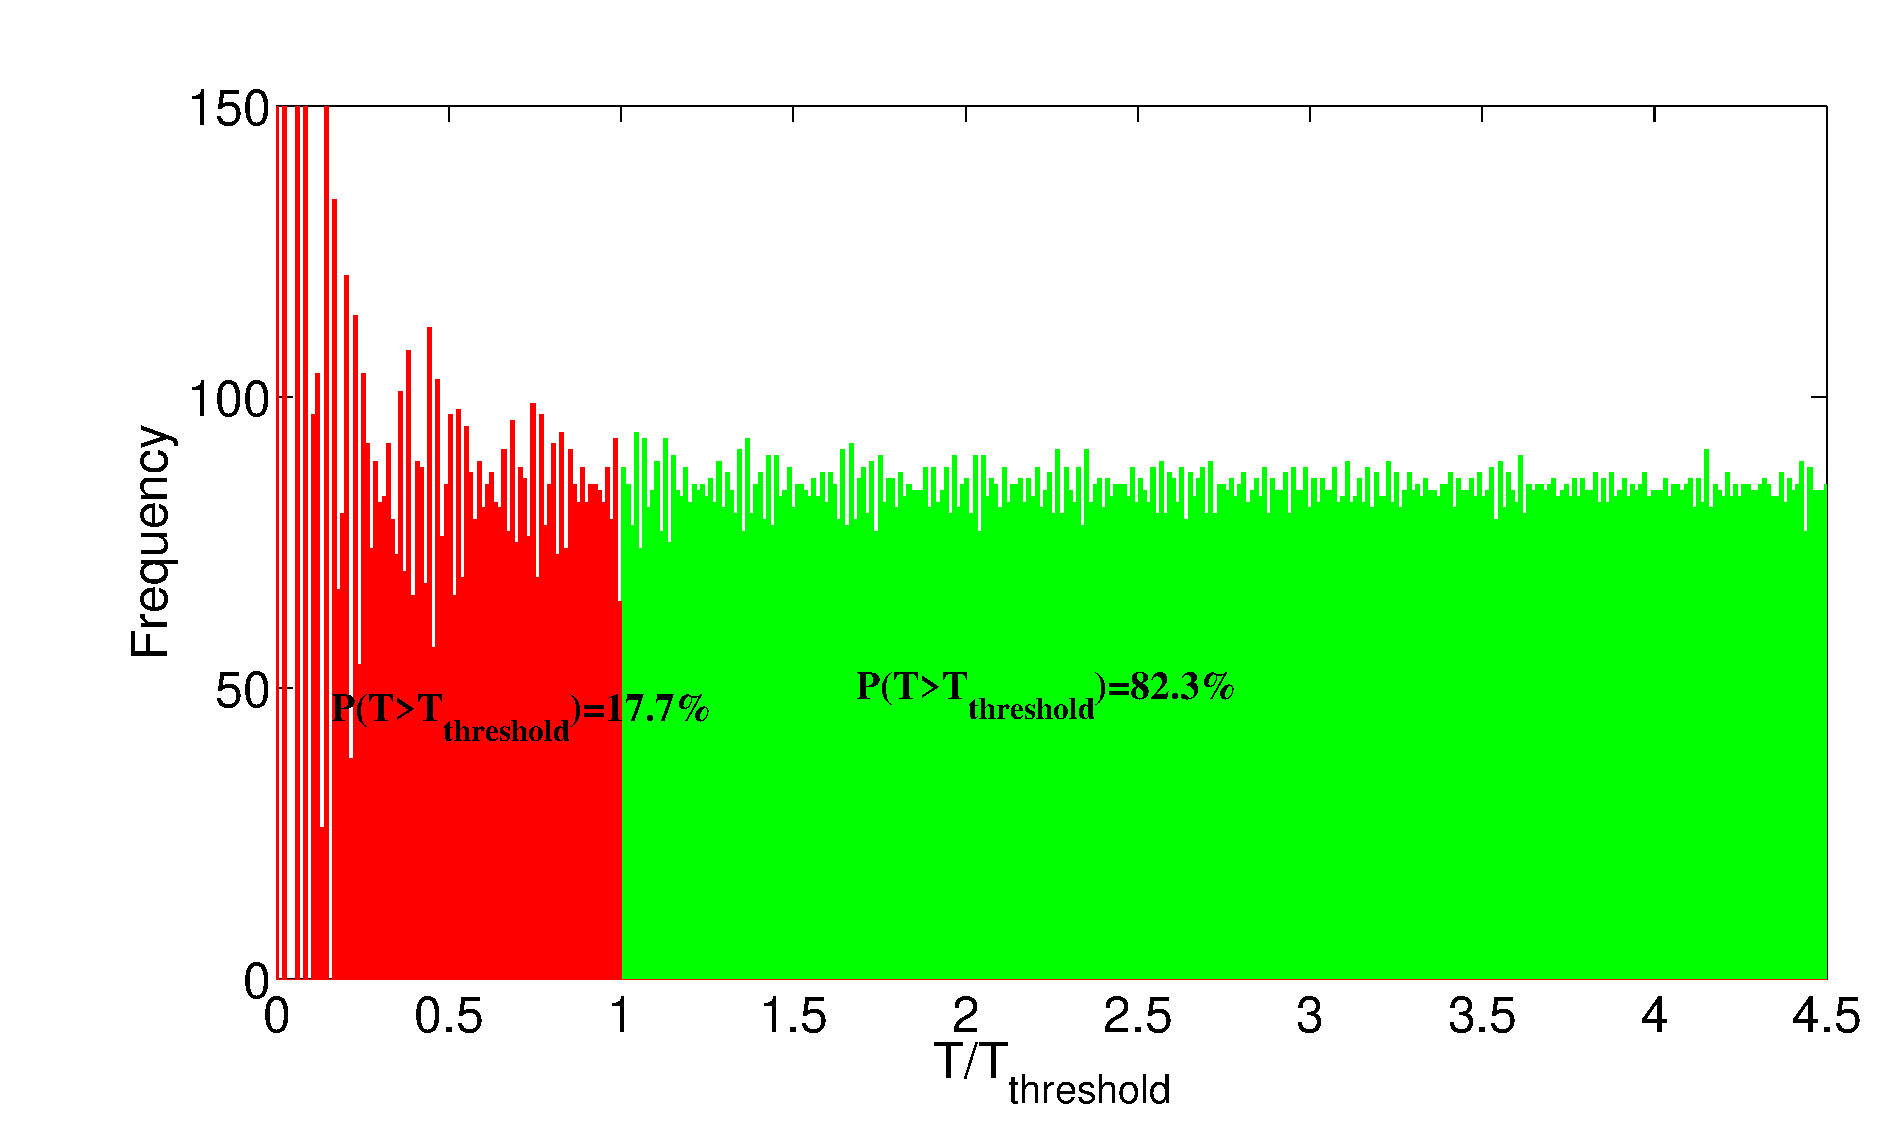
\includegraphics[width=5in]{figures/F89mhist.eps}
\caption{Histogram of the total thrombin as reaction rate $k_{14}$
and factor X is introduced. The probability that the total thrombin
is greater than $T_{threshold}$ is increased to
82.3\%.}\label{Fig:F89mhist}
  \end{center}
\end{figure}
\begin{figure}
  \begin{center}


   \includegraphics[width=5in,height=3.5in]{figures/NSAD.eps}
\caption{ Network graph of importance of reaction rates and the
interaction between pair components with respect to total thrombin
when blocking $k_{14}$ and $k_{15}$ (their values are reduced by
90\%). See the legend in Figure 1. This figure shows that the
sensitivity shifts, i.e., reaction rate $k_{23}$ becomes the most
sensitive reaction rates in activating thrombin when $k_{14}$ and
$k_{25}$ are blocked. Moreover, $k_{13}$ plays no roles since
chemical reaction with $k_{13}$ is combined with $k_{14}$ and
$k_{25}$. }\label{Fig:NSAD}
  \end{center}
\end{figure}


\begin{table}
\section*{APPENDIX A}
Chemical equations
\begin{center}
 \caption{Chemical expressions for the coagulation cascade}\label{taba}
 \vspace{3mm}
\begin{tabular}{|c|c|}\hline
Line&Chemical expressions\\\hline
  1& TF + VII $<1-2>$ TF=VII\\\hline
  2& TF + VIIa $<3-4>$ TF=VIIa\\\hline
 3 & TF=VIIa + VII $ -5>$ TF=VIIa + VIIa  \\\hline
 4 & Xa + VII $-6>$ Xa +
VIIa \\\hline
  5 & IIa + VII $-7>$ IIa + VIIa \\\hline
  6 &TF=VIIa + X  $<8-9>$ TF=VIIa=X $-10>$ TF=VIIa=Xa\\\hline
7 & TF=VIIa +Xa $<11-12>$ TF=VIIa=Xa\\\hline
 8 &TF=VIIa + IX $<13-14>$ TF=VIIa=IX $-15>$ TF=VIIa + IXa\\\hline
  9& Xa + II $-16>$ Xa +IIa \\\hline
  10& IIa + VIII $-17>$ IIa + VIIIa \\\hline
  11& VIIIa + IXa $<18-19>$ IXa=VIIIa \\\hline
  12 & IXa=VIIIa +  X $<20-21>$ IXa=VIIIa=X $-22>$ IXa=VIIIa +
  Xa\\\hline
13 & VIIIa $<23-24>$ VIII$a_1\cdot$ L +  VIII$a_2$\\\hline 14&
IXa=VIIIa=X $-25>$ VIII$a_1\cdot$ L + VIII$a_2$ + X +IXa\\\hline
 15& IXa=VIIIa $-25>$ VIII$a_1\cdot$ L VIII$a_2$ +IXa\\\hline
  16& IIa+ V $-26>$ IIa +Va\\\hline
   17 &Xa + Va $<27-28>$ Xa=Va \\\hline
   18& Xa=Va + II $<29-30>$ Xa=Va=II $-31>$ Xa=Va + mIIa\\\hline
    19& mIIa+ Xa=Va $-32>$ IIa + Xa=Va \\\hline
    20& Xa + TFPI $<33-34>$ Xa=TFPI \\\hline
    21& TF=VIIa=Xa + TFPI $<35-36>$ TF=VIIa=Xa=TFPI \\\hline
    22 & TF=VIIa + Xa=TFPI $-37>$ TF=VIIa=Xa=TFPI \\\hline
    23& Xa+ATIII $-38>$ Xa=ATIII\\\hline
     24& mIIa+ ATIII $-39>$ mIIa=ATIII\\\hline
      25& IXa + ATIII $-40>$ IXa=ATIII\\\hline
26& IIa + ATIII $-41>$ IIa=ATIII\\\hline
 27& TF=VIIa + ATIII $-42>$TF=VIIa=ATIII\\\hline
\end{tabular}

\caption{ Variables and Species} \label{tabb} \vspace{3mm}
\begin{tabular}{|c|c|c|c|c|c|c|c|}\cline{1-2}
\cline{4-5}\cline{7-8} $x_{1}
$&TF&&$x_{13}$&IIa&&$x_{25}$&IXa\\\cline{1-2}\cline{4-5}\cline{7-8}
$x_{2}
$&IXa=VIIIa=X&&$x_{14}$&Xa=Va=II&&$x_{26}$&Xa=ATIII\\\cline{1-2}\cline{4-5}\cline{7-8}
$x_{3}
$&VII&&$x_{15}$&X&&$x_{27}$&II\\\cline{1-2}\cline{4-5}\cline{7-8}
$x_{4} $&VIII$a_1\cdot$
L&&$x_{16}$&mIIa&&$x_{28}$&mIIa=ATIII\\\cline{1-2}\cline{4-5}\cline{7-8}
$x_{5}
$&TF=VII&&$x_{17}$&TF=VIIa=X&&$x_{29}$&VIII\\\cline{1-2}\cline{4-5}\cline{7-8}
$x_{6}
$&VIII$a_2$&&$x_{18}$&TFPI&&$x_{30}$&IXa=ATIII\\\cline{1-2}\cline{4-5}\cline{7-8}
$x_{7}
$&VIIa&&$x_{19}$&TF=VIIa=Xa&&$x_{31}$&VIIIa\\\cline{1-2}\cline{4-5}\cline{7-8}
$x_{8}
$&V&&$x_{20}$&Xa=TFPI&&$x_{32}$&IIa=ATIII\\\cline{1-2}\cline{4-5}\cline{7-8}
$x_{9}
$&TF=VIIa&&$x_{21}$&IX&&$x_{33}$&IXa=VIIIa\\\cline{1-2}\cline{4-5}\cline{7-8}
$x_{10}$&Va&&$x_{22}$&TF=VIIa=Xa=TFPI&&$x_{34}$&TF=VIIa=ATIII\\\cline{1-2}\cline{4-5}\cline{7-8}
$x_{11}$&Xa&&$x_{23}$&TF=VIIa=IX&&$
$&\\\cline{1-2}\cline{4-5}\cline{7-8}
$x_{12}$&Xa=Va&&$x_{24}$&ATIII&&$
$&\\\cline{1-2}\cline{4-5}\cline{7-8}
\end{tabular}
\end{center}
\end{table}

\clearpage
\section*{APPENDIX B}
Model equations
 \bes
\frac{dx_{1}}{dt} &=& -k_{2} x_{1} x_{2}+k_{1} x_{3}-k_{4} x_{1}
x_{4}+k_{3} x_{5},\quad
\frac{dx_{2}}{dt} = -k_{2} x_{1} x_{2}+k_{1} x_{3}-k_{5} x_{5} x_{2}-k_{6} x_{6} x_{2}-k_{7} x_{7} x_{2}\nnu\\
\frac{dx_{3}}{dt} &=& k_{2} x_{1} x_{2}-k_{1} x_{3}, \quad\quad\quad\quad \quad\quad\quad \frac{dx_{4}}{dt} = -k_{4} x_{1} x_{4}+k_{3} x_{5}+k_{5} x_{5} x_{2}+k_{6} x_{6} x_{2}+k_{7} x_{7} x_{2}\nnu\\
\frac{dx_{5}}{dt} &=& k_{4} x_{1} x_{4}-k_{3} x_{5}-k_{9} x_{5}
x_{8}+k_{8} x_{9}-k_{12} x_{5} x_{6}+k_{11} x_{10}-k_{14} x_{5}
x_{11}+k_{13} x_{12}-k_{37} x_{5} x_{27}\nnu\\
&\ &-k_{42} x_{5} x_{29}+k_{15} x_{12}\nnu\\
\frac{dx_{6}}{dt} &=& -k_{12} x_{5} x_{6}+k_{11} x_{10}-k_{28} x_{6} x_{22}+k_{27} x_{23}-k_{34} x_{6} x_{26}+k_{33} x_{27}-k_{38} x_{6} x_{29}+k_{22} x_{18}\nnu\\
\frac{dx_{7}}{dt} &=& k_{16} x_{6} x_{14}+k_{32} x_{25}
x_{23}-k_{41} x_{7} x_{29},\quad
\frac{dx_{8}}{dt} = -k_{9} x_{5} x_{8}+k_{8} x_{9}-k_{21} x_{17} x_{8}+k_{20} x_{18}+k_{25} x_{18}\nnu\\
\frac{dx_{9}}{dt} &=& k_{9} x_{5} x_{8}-k_{8} x_{9}-k_{10}
x_{9},\quad\quad\quad\frac{dx_{10}}{dt} = k_{12} x_{5} x_{6}-k_{11} x_{10}-k_{36} x_{10} x_{26}+k_{35} x_{28}+k_{10} x_{9}\nnu\\
\frac{dx_{11}}{dt} &=& -k_{14} x_{5} x_{11}+k_{13}
x_{12},\quad\quad\quad\quad\frac{dx_{12}}{dt} = k_{14} x_{5}
x_{11}-k_{13} x_{12}-k_{15}
x_{12}\nnu\\
\frac{dx_{13}}{dt} &=& -k_{19} x_{16} x_{13}+k_{18} x_{17}+k_{25}
x_{18}+k_{25} x_{17}-k_{40} x_{13} x_{29}+k_{15} x_{12}\nnu\\
\frac{dx_{14}}{dt} &=& -k_{16} x_{6} x_{14}-k_{30} x_{23}
x_{14}+k_{29} x_{24}\nnu\\ \frac{dx_{15}}{dt} &=& -k_{17} x_{7}
x_{15},\quad\quad\quad\quad\quad\frac{dx_{16}}{dt} = k_{17} x_{7}
x_{15}-k_{19}
x_{16} x_{13}+k_{18} x_{17}-k_{24} x_{16}+k_{23} x_{19} x_{20}\nnu\\
\frac{dx_{17}}{dt} &=& k_{19} x_{16} x_{13}-k_{18} x_{17}-k_{21}
x_{17} x_{8}+k_{20} x_{18}-k_{25} x_{17}+k_{22} x_{18}\nnu\\
\frac{dx_{18}}{dt} &=& k_{21} x_{17} x_{8}-k_{20} x_{18}-k_{25} x_{18}-k_{22} x_{18}\nnu\\
\frac{dx_{19}}{dt} &=& \frac{dx_{20}}{dt} ~=~ k_{24} x_{16}-k_{23} x_{19} x_{20}+k_{25} x_{18}+k_{25} x_{17}\nnu\\
\frac{dx_{21}}{dt} &=& -k_{26} x_{7} x_{21}\quad\quad\quad\quad\quad\quad\frac{dx_{22}}{dt} = k_{26} x_{7} x_{21}-k_{28} x_{6} x_{22}+k_{27} x_{23}\nnu\\
\frac{dx_{23}}{dt} &=& k_{28} x_{6} x_{22}-k_{27} x_{23}-k_{30}
x_{23} x_{14}+k_{29} x_{24}+k_{31} x_{24}\nnu\\
\frac{dx_{24}}{dt} &=& k_{30} x_{23} x_{14}-k_{29} x_{24}-k_{31}
x_{24},\quad\quad\frac{dx_{25}}{dt} = -k_{32} x_{25} x_{23}-k_{39}
x_{25} x_{29}+k_{31} x_{24}\nnu\\\frac{dx_{26}}{dt} &=& -k_{34}
x_{6}
x_{26}+k_{33} x_{27}-k_{36} x_{10} x_{26}+k_{35} x_{28}\nnu \\
\frac{dx_{27}}{dt} &=& k_{34}
x_{6} x_{26}-k_{33} x_{27}-k_{37} x_{5} x_{27},\quad\quad\frac{dx_{28}}{dt} = k_{36} x_{10} x_{26}-k_{35} x_{28}+k_{37} x_{5} x_{27}\nnu\\
\frac{dx_{29}}{dt} &=& -k_{38} x_{6} x_{29}-k_{39} x_{25} x_{29}-k_{40} x_{13} x_{29}-k_{41} x_{7} x_{29}-k_{42} x_{5} x_{29}\quad\quad\quad\frac{dx_{30}}{dt} = k_{38} x_{6} x_{29}\nnu\\
\frac{dx_{31}}{dt} &=& k_{39} x_{25}
x_{29},\quad\quad\frac{dx_{32}}{dt} = k_{40} x_{13}
x_{29},\quad\quad\quad\frac{dx_{33}}{dt} = k_{41} x_{7}
x_{29},\quad\quad\quad\frac{dx_{34}}{dt} = k_{42} x_{5}
x_{29}\label{1},\ees where $k_i,i=1,2,...,42$ are constants, and
$x_i,i=1,2,...,34$ are variables representing the species (see
Table~\ref{tabb}). The steady state system can be obtained by taking
$t\rightarrow \infty$, i.e., $\frac{dx_i}{dt}=0,\forall i$.



\section*{APPENDIX C}
\bes f_{1} &=& -k_{4} x_{1} x_{4}+k_{3} x_{5}\nnu\\
f_{2} &=& -k_{5} x_{5} x_{2}-k_{6} x_{6} x_{2}-k_{7} x_{7} x_{2}\nnu\\
f_{3} &=& k_{2} x_{1} x_{2}-k_{1} x_{3}\nnu\\
f_{4} &=& -k_{12} x_{5} x_{6}-k_{42} x_{5} x_{29}+k_{4} x_{1} x_{4}-k_{3} x_{5}+k_{8} x_{9}-k_{9} x_{5} x_{8}+k_{11} x_{10}-k_{37} x_{5} x_{27}\nnu\\
f_{5} &=& -k_{12} x_{5} x_{6}-k_{34} x_{6} x_{26}+k_{11} x_{10}+k_{33} x_{27}-k_{38} x_{6} x_{29}+k_{22} x_{18}\nnu\\
f_{6} &=& k_{16} x_{6} x_{14}+k_{32} x_{25} x_{23}-k_{41} x_{7} x_{29}\nnu\\
f_{7} &=& -k_{9} x_{5} x_{8}+k_{8} x_{9}-k_{21} x_{17} x_{8}+k_{20} x_{18}+k_{25} x_{18}\nnu\\
f_{8} &=& k_{9} x_{5} x_{8}-k_{8} x_{9}-k_{10} x_{9}\nnu\\
f_{9} &=& k_{12} x_{5} x_{6}-k_{11} x_{10}-k_{36} x_{10} x_{26}+k_{35} x_{28}+k_{10} x_{9}\nnu\\
f_{10} &=& -k_{14} x_{5} x_{11}+k_{13} x_{12}\nnu\\
f_{11} &=& -k_{15} x_{12}\nnu\\
f_{12} &=& -k_{19} x_{16} x_{13}+k_{18} x_{17}+k_{25} x_{18}+k_{25} x_{17}-k_{40} x_{13} x_{29}\nnu\\
f_{13} &=& -k_{16} x_{6} x_{14}-k_{30} x_{23} x_{14}+k_{29} x_{24}\nnu\\
f_{14} &=& -k_{17} x_{7} x_{15}\nnu\\
f_{15} &=& -k_{19} x_{16} x_{13}+k_{18} x_{17}-k_{24} x_{16}+k_{23} x_{19} x_{20}\nnu\\
f_{16} &=& k_{19} x_{16} x_{13}-k_{18} x_{17}-k_{21} x_{17}
x_{8}+k_{20} x_{18}-k_{25} x_{17}+k_{22} x_{18}\nnu\\
f_{17} &=& k_{21} x_{17} x_{8}-k_{20} x_{18}-k_{25} x_{18}-k_{22} x_{18}\nnu\\
f_{18} &=& -k_{26} x_{7} x_{21}\nnu\\
f_{19} &=& -k_{28} x_{6} x_{22}+k_{27} x_{23}\nnu\\
f_{20} &=& k_{29} x_{24}-k_{30} x_{23} x_{14}+k_{31} x_{24}\nnu\\
f_{21} &=& -k_{32} x_{25} x_{23}+k_{31} x_{24}\nnu\\
f_{22} &=& -k_{34} x_{6} x_{26}+k_{33} x_{27}-k_{36} x_{10} x_{26}+k_{35} x_{28}\nnu\\
f_{23} &=& k_{34} x_{6} x_{26}-k_{33} x_{27}-k_{37} x_{5} x_{27}\nnu\\
f_{24} &=& k_{39} x_{25} x_{29},\nnu\ees The next 10 rows can be
expressed as:
 \bes
A_{4}&=&A_{1}-A_{2}\nnu\\
A_{19}&=&-A_{15}-A_{16}-A_{17}-A_{18}\nnu\\
A_{20}&=&-A_{15}-A_{16}-A_{17}-A_{18}\nnu\\
A_{24}&=&-A_{21}-A_{22}-A_{23}\nnu\\
A_{28}&=&-A_{26}-A_{27}\nnu\\
A_{29}&=&A_{1}+A_{3}+A_{5}+A_{6}+A_{7}+A_{8}+2A_{9}+2A_{10}+A_{11}+2A_{12}+A_{13}+A_{14}+A_{17}+2A_{18}\nnu\\
&\ &-2A_{21}-2A_{22}-A_{23}+A_{25}-2A_{26}-A_{27}\nnu\\
A_{30}&=&-A_{6}-A_{8}-A_{9}-A_{10}-A_{18}+A_{21}+A_{22}+A_{26}\nnu\\
A_{32}&=&-A_{11}-A_{12}-A_{13}-A_{17}\nnu\\
A_{33}&=&-A_{7}-A_{14}+A_{21}+A_{22}+A_{23}-A_{25}-A_{31}\nnu\\
A_{34}&=&-A_{1}-A_{3}-A_{5}-A_{9}-A_{10}-A_{12}+A_{26}+A_{27},\nnu
\ees where $A_i,~ i=1,2,\dots,34$ represents the $i$-th row of $A$.
\section*{APPENDIX D}
The linearized system of differential equation system shown in
Appendix B:
\bes{{x^1}_{1}}_t&=&-k_{2}{x^s}_{1}{x^1}_{2}-k_{2}{x^1}_{1}{x^s}_{2}+k_{1}{x^1}_{3}-k_{4}{x^s}_{1}{x^1}_{4}-k_{4}{x^1}_{1}{x^s}_{4}+k_{3}{x^1}_{5}\nnu\\
{{x^1}_{2}}_t&=&-k_{2}{x^s}_{1}{x^1}_{2}-k_{2}{x^1}_{1}{x^s}_{2}+k_{1}{x^1}_{3}-k_{5}{x^s}_{5}{x^1}_{2}-k_{5}{x^1}_{5}{x^s}_{2}-k_{6}{x^s}_{6}{x^1}_{2}-k_{6}{x^1}_{6}{x^s}_{2}\nnu\\
&\ &-k_{7}{x^s}_{7}{x^1}_{2}-k_{7}{x^1}_{7}{x^s}_{2}\nnu\\
{{x^1}_{3}}_t&=&k_{2}{x^s}_{1}{x^1}_{2}+k_{2}{x^1}_{1}{x^s}_{2}-k_{1}{x^1}_{3}\nnu\\
{{x^1}_{4}}_t&=&-k_{4}{x^s}_{1}{x^1}_{4}-k_{4}{x^1}_{1}{x^s}_{4}+k_{3}{x^1}_{5}+k_{5}{x^s}_{5}{x^1}_{2}+k_{5}{x^1}_{5}{x^s}_{2}+k_{6}{x^s}_{6}{x^1}_{2}+k_{6}{x^1}_{6}{x^s}_{2}\nnu\\
&\ &+k_{7}{x^s}_{7}{x^1}_{2}+k_{7}{x^1}_{7}{x^s}_{2}\nnu\\
{{x^1}_{5}}_t&=&k_{8}{x^1}_{9}+k_{4}{x^s}_{1}{x^1}_{4}+k_{4}{x^1}_{1}{x^s}_{4}+k_{13}{x^1}_{12}+k_{11}{x^1}_{10}-k_{3}{x^1}_{5}-k_{9}{x^s}_{5}{x^1}_{8}-k_{9}{x^1}_{5}{x^s}_{8}\nnu\\
&\ &-k_{12}{x^s}_{5}{x^1}_{6}-k_{12}{x^1}_{5}{x^s}_{6}-k_{14}{x^s}_{5}{x^1}_{11}-k_{14}{x^1}_{5}{x^s}_{11}-k_{37}{x^s}_{5}{x^1}_{27}-k_{37}{x^1}_{5}{x^s}_{27}\nnu\\
&\ &-k_{42}{x^s}_{5}{x^1}_{29}-k_{42}{x^1}_{5}{x^s}_{29}+k_{15}{x^1}_{12}\nnu\\
{{x^1}_{6}}_t&=&k_{33}{x^1}_{27}+k_{27}{x^1}_{23}+k_{22}{x^1}_{18}+k_{11}{x^1}_{10}-k_{12}{x^s}_{5}{x^1}_{6}-k_{12}{x^1}_{5}{x^s}_{6}-k_{28}{x^s}_{6}{x^1}_{22}\nnu\\
&\ &-k_{28}{x^1}_{6}{x^s}_{22}-k_{34}{x^s}_{6}{x^1}_{26}-k_{34}{x^1}_{6}{x^s}_{26}-k_{38}{x^s}_{6}{x^1}_{29}-k_{38}{x^1}_{6}{x^s}_{29}\nnu\\
{{x^1}_{7}}_t&=&k_{16}{x^s}_{6}{x^1}_{14}+k_{16}{x^1}_{6}{x^s}_{14}+k_{32}{x^s}_{25}{x^1}_{23}+k_{32}{x^1}_{25}{x^s}_{23}-k_{41}{x^s}_{7}{x^1}_{29}-k_{41}{x^1}_{7}{x^s}_{29}\nnu\\
{{x^1}_{8}}_t&=&-k_{9}{x^s}_{5}{x^1}_{8}-k_{9}{x^1}_{5}{x^s}_{8}+k_{8}{x^1}_{9}-k_{21}{x^s}_{17}{x^1}_{8}-k_{21}{x^1}_{17}{x^s}_{8}+k_{20}{x^1}_{18}+k_{25}{x^1}_{18}\nnu\\
{{x^1}_{9}}_t&=&k_{9}{x^s}_{5}{x^1}_{8}+k_{9}{x^1}_{5}{x^s}_{8}-k_{8}{x^1}_{9}-k_{10}{x^1}_{9}\nnu\\
{{x^1}_{10}}_t&=&k_{12}{x^s}_{5}{x^1}_{6}+k_{12}{x^1}_{5}{x^s}_{6}-k_{11}{x^1}_{10}-k_{36}{x^s}_{10}{x^1}_{26}-k_{36}{x^1}_{10}{x^s}_{26}+k_{35}{x^1}_{28}+k_{10}{x^1}_{9}\nnu\\
{{x^1}_{11}}_t&=&-k_{14}{x^s}_{5}{x^1}_{11}-k_{14}{x^1}_{5}{x^s}_{11}+k_{13}{x^1}_{12}\nnu\\
{{x^1}_{12}}_t&=&k_{14}{x^s}_{5}{x^1}_{11}+k_{14}{x^1}_{5}{x^s}_{11}-k_{13}{x^1}_{12}-k_{15}{x^1}_{12}\nnu\\
{{x^1}_{13}}_t&=&-k_{19}{x^s}_{16}{x^1}_{13}-k_{19}{x^1}_{16}{x^s}_{13}+k_{18}{x^1}_{17}+k_{25}{x^1}_{18}+k_{25}{x^1}_{17}-k_{40}{x^s}_{13}{x^1}_{29}-k_{40}{x^1}_{13}{x^s}_{29}\nnu\\
&\ &+k_{15}{x^1}_{12}\nnu\\
{{x^1}_{14}}_t&=&-k_{16}{x^s}_{6}{x^1}_{14}-k_{16}{x^1}_{6}{x^s}_{14}-k_{30}{x^s}_{23}{x^1}_{14}-k_{30}{x^1}_{23}{x^s}_{14}+k_{29}{x^1}_{24}\nnu\\
{{x^1}_{15}}_t&=&-k_{17}({x^s}_{7}{x^1}_{15}+{x^1}_{7}{x^s}_{15})\nnu\\
{{x^1}_{16}}_t&=&k_{17}{x^s}_{7}{x^1}_{15}+k_{17}{x^1}_{7}{x^s}_{15}-k_{19}{x^s}_{16}{x^1}_{13}-k_{19}{x^1}_{16}{x^s}_{13}+k_{18}{x^1}_{17}-k_{24}{x^1}_{16}+k_{23}{x^s}_{19}{x^1}_{20}\nnu\\
&\ &+k_{23}{x^1}_{19}{x^s}_{20}\nnu\\
{{x^1}_{17}}_t&=&k_{19}{x^s}_{16}{x^1}_{13}+k_{19}{x^1}_{16}{x^s}_{13}-k_{18}{x^1}_{17}-k_{21}{x^s}_{17}{x^1}_{8}-k_{21}{x^1}_{17}{x^s}_{8}+k_{20}{x^1}_{18}-k_{25}{x^1}_{17}\nnu\\
&\ &+k_{22}{x^1}_{18}\nnu \ees\bes
{{x^1}_{18}}_t&=&k_{21}{x^s}_{17}{x^1}_{8}+k_{21}{x^1}_{17}{x^s}_{8}-k_{20}{x^1}_{18}-k_{25}{x^1}_{18}-k_{22}{x^1}_{18}\nnu\\
{{x^1}_{19}}_t&=&k_{24}{x^1}_{16}-k_{23}{x^s}_{19}{x^1}_{20}-k_{23}{x^1}_{19}{x^s}_{20}+k_{25}{x^1}_{18}+k_{25}{x^1}_{17}\nnu\\
{{x^1}_{20}}_t&=&k_{24}{x^1}_{16}-k_{23}{x^s}_{19}{x^1}_{20}-k_{23}{x^1}_{19}{x^s}_{20}+k_{25}{x^1}_{18}+k_{25}{x^1}_{17}\nnu\\
{{x^1}_{21}}_t&=&-k_{26}({x^s}_{7}{x^1}_{21}+{x^1}_{7}{x^s}_{21})\nnu\\
{{x^1}_{22}}_t&=&k_{26}{x^s}_{7}{x^1}_{21}+k_{26}{x^1}_{7}{x^s}_{21}-k_{28}{x^s}_{6}{x^1}_{22}-k_{28}{x^1}_{6}{x^s}_{22}+k_{27}{x^1}_{23}\nnu\\
{{x^1}_{23}}_t&=&k_{28}{x^s}_{6}{x^1}_{22}+k_{28}{x^1}_{6}{x^s}_{22}-k_{27}{x^1}_{23}-k_{30}{x^s}_{23}{x^1}_{14}-k_{30}{x^1}_{23}{x^s}_{14}+k_{29}{x^1}_{24}+k_{31}{x^1}_{24}\nnu\\
{{x^1}_{24}}_t&=&k_{30}{x^s}_{23}{x^1}_{14}+k_{30}{x^1}_{23}{x^s}_{14}-k_{29}{x^1}_{24}-k_{31}{x^1}_{24}\nnu\\
{{x^1}_{25}}_t&=&-k_{32}{x^s}_{25}{x^1}_{23}-k_{32}{x^1}_{25}{x^s}_{23}-k_{39}{x^s}_{25}{x^1}_{29}-k_{39}{x^1}_{25}{x^s}_{29}+k_{31}{x^1}_{24}\nnu\\
{{x^1}_{26}}_t&=&-k_{34}{x^s}_{6}{x^1}_{26}-k_{34}{x^1}_{6}{x^s}_{26}+k_{33}{x^1}_{27}-k_{36}{x^s}_{10}{x^1}_{26}-k_{36}{x^1}_{10}{x^s}_{26}+k_{35}{x^1}_{28}\nnu\\
{{x^1}_{27}}_t&=&k_{34}{x^s}_{6}{x^1}_{26}+k_{34}{x^1}_{6}{x^s}_{26}-k_{33}{x^1}_{27}-k_{37}{x^s}_{5}{x^1}_{27}-k_{37}{x^1}_{5}{x^s}_{27}\nnu\\
{{x^1}_{28}}_t&=&k_{36}{x^s}_{10}{x^1}_{26}+k_{36}{x^1}_{10}{x^s}_{26}-k_{35}{x^1}_{28}+k_{37}{x^s}_{5}{x^1}_{27}+k_{37}{x^1}_{5}{x^s}_{27}\nnu\\
{{x^1}_{29}}_t&=&-k_{42}{x^s}_{5}{x^1}_{29}-k_{42}{x^1}_{5}{x^s}_{29}-k_{38}{x^s}_{6}{x^1}_{29}-k_{38}{x^1}_{6}{x^s}_{29}-k_{41}{x^s}_{7}{x^1}_{29}\nnu\\
&\ &-k_{41}{x^1}_{7}{x^s}_{29}-k_{40}{x^s}_{13}{x^1}_{29}-k_{40}{x^1}_{13}{x^s}_{29}-k_{39}{x^s}_{25}{x^1}_{29}-k_{39}{x^1}_{25}{x^s}_{29}\nnu\\
{{x^1}_{30}}_t&=&k_{38}({x^s}_{6}{x^1}_{29}+{x^1}_{6}{x^s}_{29})\nnu\\
{{x^1}_{31}}_t&=&k_{39}({x^s}_{25}{x^1}_{29}+{x^1}_{25}{x^s}_{29})\nnu\\
{{x^1}_{32}}_t&=&k_{40}({x^s}_{13}{x^1}_{29}+{x^1}_{13}{x^s}_{29})\nnu\\
{{x^1}_{33}}_t&=&k_{41}({x^s}_{7}{x^1}_{29}+{x^1}_{7}{x^s}_{29})\nnu\\
{{x^1}_{34}}_t&=&k_{42}({x^s}_{5}{x^1}_{29}+{x^1}_{5}{x^s}_{29})\nnu\ees
\clearpage
\section*{Appendix E}
\begin{table}[!ht]
\begin{center}
\caption{Convergence study of SGPCM}\vspace{3mm} \label{conv}
\begin{tabular}{|c|c|c|c|c|}\hline
\multicolumn{5}{|c|}{Abs. Err.}\\\hline &\multicolumn{2}{|c|}{Mean}
& \multicolumn{2}{|c|}{ Variance}\\\hline No. & 184 &    1228     &
184 & 1228\\\hline 1 & 2.285678e-004&6.276008e-005
&1.414116e+000&5.270631e-001\\\hline 2 & 3.528170e-003&9.790568e-004
&1.421438e+000&5.282797e-001\\\hline 3 & 1.117445e-002&3.058945e-003
&1.451133e+000&5.334394e-001\\\hline 4 & 1.737843e-004&4.822458e-005
&1.421425e+000&5.282775e-001\\\hline 5 & 8.828347e-003&2.389501e-003
&1.486561e+000&5.391973e-001\\\hline 6 & 1.988338e-002&5.317003e-003
&1.566493e+000&5.520586e-001\\\hline 7 & 4.584148e-003&1.255587e-003
&1.427882e+000&5.293661e-001\\\hline 8 & 2.048073e-004&5.578918e-005
&1.454606e+000&5.339573e-001\\\hline 9 & 3.396093e-003&9.241881e-004
&1.424554e+000&5.287619e-001\\\hline 10 &
3.256174e-003&8.869390e-004 &1.423624e+000&5.286163e-001\\\hline 11
& 8.412776e-006&2.279950e-006 &1.480436e+000&5.382099e-001\\\hline
12 & 8.808674e-003&2.384262e-003
&1.486394e+000&5.391702e-001\\\hline 13 &
8.277039e-003&2.243433e-003 &1.479954e+000&5.381284e-001\\\hline 14
& 3.103763e-003&8.465279e-004 &1.443678e+000&5.320069e-001\\\hline
15 & 7.814273e-003&2.193114e-003
&1.426201e+000&5.286388e-001\\\hline 16 &
1.328375e-002&3.739625e-003 &1.415327e+000&5.270061e-001\\\hline 17
& 9.094976e-003&2.458848e-003 &1.490370e+000&5.397825e-001\\\hline
18 & 8.172212e-003&2.212621e-003
&1.483100e+000&5.386074e-001\\\hline 19 &
2.363583e-003&6.446736e-004 &1.460426e+000&5.347973e-001\\\hline 20
& 2.363583e-003&6.446736e-004 &1.460426e+000&5.347973e-001\\\hline
21 & 7.814273e-003&2.193114e-003
&1.426201e+000&5.286388e-001\\\hline 22 &
7.593356e-003&2.131857e-003 &1.425644e+000&5.288239e-001\\\hline 23
& 2.706446e-003&7.513140e-004 &1.429067e+000&5.297737e-001\\\hline
24 & 1.078126e-002&2.958615e-003
&1.431272e+000&5.298548e-001\\\hline 25 &
9.639244e-003&2.646268e-003 &1.426693e+000&5.291310e-001\\\hline 26
& 3.609443e-004&9.730916e-005 &1.492187e+000&5.400877e-001\\\hline
27 & 1.019074e-002&2.748554e-003
&1.499708e+000&5.413532e-001\\\hline 28 &
2.549383e-003&6.949484e-004 &1.420171e+000&5.280515e-001\\\hline 29
& 5.662490e-004&1.541640e-004 &1.448082e+000&5.327725e-001\\\hline
30 & 9.960178e-003&2.677646e-003
&1.508239e+000&5.426681e-001\\\hline 31 &
2.958200e-003&8.078085e-004 &1.445202e+000&5.322928e-001\\\hline 32
& 7.845463e-003&2.126566e-003 &1.478513e+000&5.378746e-001\\\hline
33 & 2.120963e-003&5.769229e-004
&1.427220e+000&5.293214e-001\\\hline 34 &
8.380451e-003&2.269408e-003 &1.483615e+000&5.387117e-001\\\hline
\end{tabular}
\end{center}
\end{table}



\end{bmcformat}
\end{document}
